\documentclass[12pt,openany]{book}

\usepackage{amsmath,amssymb,amsthm}
\usepackage{graphics,epsfig,psfrag}
\usepackage{tikz}

\usepackage{makeidx}
\makeindex

\usepackage[hyperindex]{hyperref}

\topmargin          0.0in
\headheight         0.25in
\headsep            0.25in
\oddsidemargin      0.5in
\evensidemargin     0.5in
\textheight         8.5in
\textwidth          5.5in

\newtheorem{theorem}{Theorem}[section]
\newtheorem{proposition}[theorem]{Proposition}
\newtheorem{definition}[theorem]{Definition}
\newtheorem{example}[theorem]{Example}

\newcommand{\SetIn}{\ensuremath{\mathrm{1\!1}}}
\newcommand{\Expect}{\ensuremath{\mathrm{E}}}
\newcommand{\Var}{\ensuremath{\mathrm{Var}}}

\newcommand{\RealNumbers}{\mathbb{R}}
\newcommand{\RationalNumbers}{\mathbb{Q}}
\newcommand{\Integers}{\mathbb{Z}}
\newcommand{\NaturalNumbers}{\mathbb{N}}

%% Definitions
%%
\renewcommand{\baselinestretch}{1.25}
\newcommand{\defn}[2]{\textbf{\textrm{#2}}\index{#1!#2}}

\begin{document}

\frontmatter

\author{
\textbf{Committers:} \\
Jean-Francois Chamberland \\
Krishna Narayanan \\
Henry Pfister}

\title{A First Course in Digital Communications}

\date{Spring 2010}

\maketitle

\chapter*{Copyright}
Copyright \copyright 2008 \\
Free Research and Education Documents

Permission is granted to copy, distribute and/or modify this document under the terms of the \emph{GNU Free Documentation License}, Version 1.2 or any later version published by the \emph{Free Software Foundation}; with no Invariant Sections, no Front-Cover Texts, and no Back-Cover Texts.
A copy of the license is included in the section entitled ``GNU Free Documentation License''.

\tableofcontents

\chapter{Preface}

These notes provide an introduction to probability.
It presents a treatment of probability concepts and techniques necessary for a basic understanding of the subject.
The notes are designed to be used in a semester course totaling 45 hours.
The reader is expected to have a basic understanding of calculus including sequences, series, derivatives and integrals.

Possessing some programming skills will also help in order to appreciate and use the computing material and examples contained in the text.
Probability theory makes predictions about experiments whose outcomes depend upon chance.
Consequently, it lends itself beautifully to the use of computers as a tool to simulate and analyze experiments.
The computer is a powerful aid in understanding basic results of probability theory, especially through imaging and graphical representation of difficult concepts.
Finally, computer programs are useful in solving problems that do not lend themselves to close-form expressions.



.

\mainmatter


\chapter{Digital Communications}
\label{chapter:DigitalComm}

The term \emph{digital communications} broadly refers to the transmission of information using digital messages or bit streams.
There are notable advantages to transmitting data  using discrete messages.
It allows for enhanced signal processing and quality control.
In particular, errors caused by noise and interference can be detected and corrected systematically.
Digital communications also make the networking of heterogeneous systems possible, with the Internet being the most obvious such example.
These advantages, and many more, explain the widespread adoption and constantly increasing popularity of digital communication systems.


\section{System Components}

A typical digital communication system can be represented by the functional block diagram depicted in Figure~\ref{figure:BlockDiagram}.
It is composed of five basic components.
The input block contains the source, which produces data (such as voice, emails, or images), and it also includes all the operations that are required to convert the original signal waveform into a format suitable for transmission.
The transmitter takes bits from the input block and sends them over a channel using electromagnetic signals, or some alternate means.
Communication channels come in many flavors.
For instance, a transmission can take place over an ethernet cable, a coaxial cable, or free space (wireless communications).
There are also more esoteric channels like a hard drive platter, a compact disc, or a memory stick.
The role of the receiver is to recover the sent message from a collection of measurements.
This unit may need to extract the signal from noise and, possibly, correct errors that may have occurred during transmission.
Finally, the output block takes the received information and puts it back into a format that is appropriate for the end-users.

\begin{figure}[htbp]
\begin{center}
\begin{psfrags}
\psfrag{I}[c]{Input}
\psfrag{O}[c]{Output}
\psfrag{T}[c]{Transmitter}
\psfrag{R}[c]{Receiver}
\psfrag{C}[c]{Channel}
\epsfig{file=Figures/diagram,width=98.7mm}
\end{psfrags}
\end{center}
\caption{A digital communication system contains five basic components.
These building blocks appear in this diagram.}
\label{figure:BlockDiagram}
\end{figure}

Figure~\ref{figure:BlockDiagram} also alludes to the natural symmetry present in digital communication systems.
Operations that take place on the transmitter side must often be undone at the destination.
As such, complementary steps are frequently studied in pairs.
Our treatment of digital communications follows this general approach.


\subsection{The Input-Output Blocks}

The role of the input block is to take information in its natural form and to convert it into a digital format.
Depending on the nature of the source, two operations may be necessary to digitize the information waveform.
\emph{Sampling} is a signal processing technique that transforms a continuous-time function to a discrete-time signal.
The conversion of a sound wave into a sequence of samples is a common application of sampling.
The second action that may be needed is \emph{quantization}, which maps a continuous-space signal into a discrete set of possible values.
The combination of these two operations will transform an analog signal into a digital message.

\begin{figure}[htbp]
\begin{center}
\begin{psfrags}
\psfrag{I}[c]{Input}
\psfrag{S}[c]{Sampling}
\psfrag{Q}[c]{Quantization}
\psfrag{E}[c]{Compression}
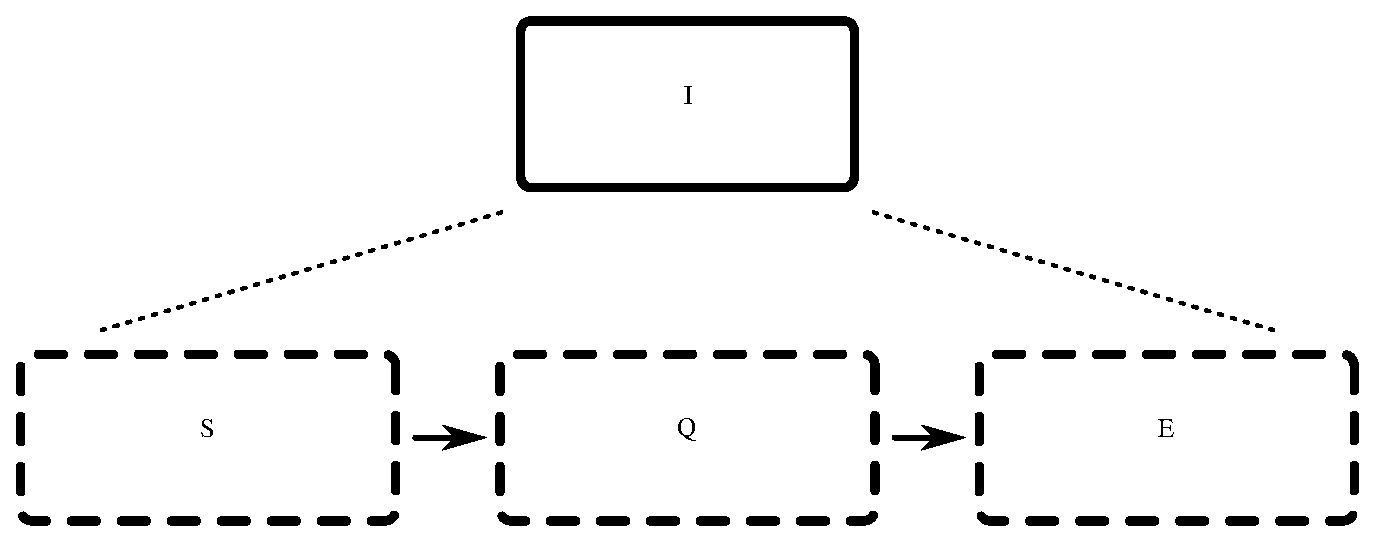
\epsfig{file=Figures/input,width=112.7mm}
\end{psfrags}
\end{center}
\caption{The input block can be further divided into three operations: sampling, quantization and data compression.
The first two operations are necessary to transform an analog waveform into a digital signal; whereas the last block is optional and provides a means to reduce the size of a digitized message.}
\label{figure:BlockInput}
\end{figure}

The optional step of \emph{data compression}, or source coding, is often employed at the origin to reduce the size of the message to be transmitted.
This, in turn, brings down the consumption of expensive resources such as power, spectral bandwidth and hard disk space.
On the downside, data processing entails additional computations and delay, and the compressed data must be expanded before being accessed.
This involves using extra processing on the receiver side as well.
Some compression schemes reduce the quality of the data.
These schemes usually feature better compression ratios at the expense of introducing small variations in the data.
The MPEG standards, including the MP3 audio layer, provide examples of lossy compression schemes.

\begin{figure}[htbp]
\begin{center}
\begin{psfrags}
\psfrag{O}[c]{Output}
\psfrag{I}[c]{Interpolation}
\psfrag{R}[c]{Reconstruction}
\psfrag{D}[c]{Decompression}
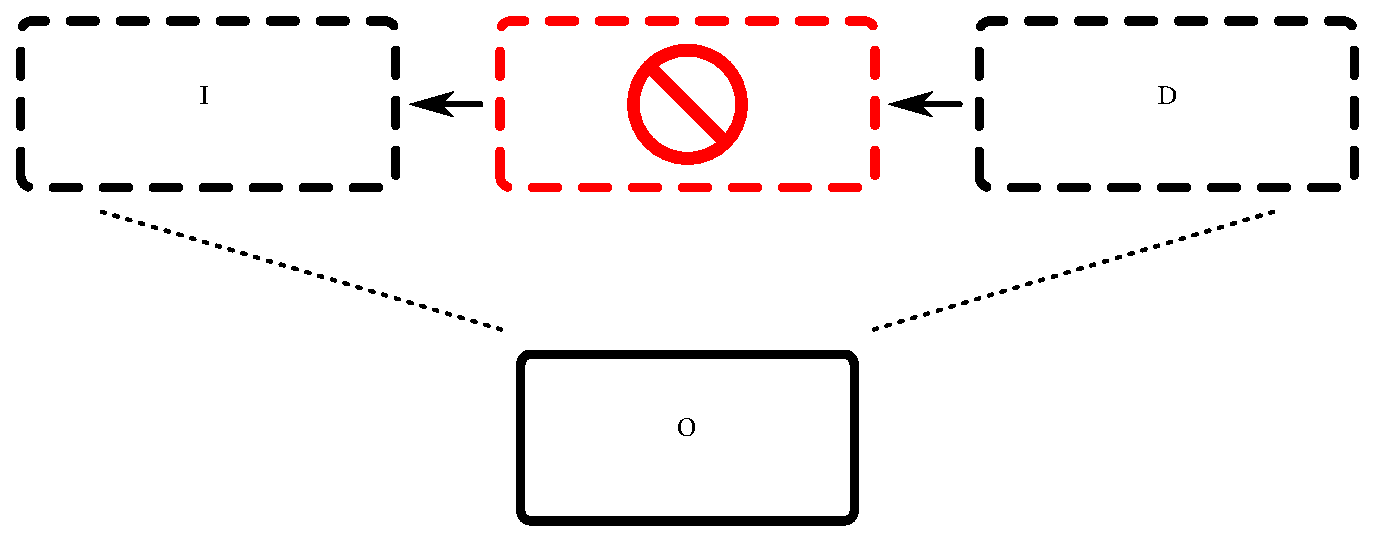
\epsfig{file=Figures/output,width=112.7mm}
\end{psfrags}
\end{center}
\caption{The operations executed at the transmitter must typically be undone at the destination.
When passed through the output block, the received data is first decompressed and put in a format that suitable for signal processing.
Furthermore, an analog signal must be reconstructed from the sampled data point.
While these two steps can reversed without any loss, the quantization step cannot.
This is because quantization loses a small part of the original information.
Instead, the reconstruction step reverses quantization step in an approximate way to minimize the distortion.}
\label{figure:BlockOutput}
\end{figure}

At the output of the system, the data must be transformed back into a format that is acceptable to the end-user.
The received message must be decompressed.
Note that for the destination to be able to recover the original data, it must understand the encoding scheme utilized by the sender.
In other words, the decoding method must be known at the receiver.
If the original signal is a continuous-time waveform, then an interpolator can be used to reconstruct the waveform from its sample values.
The quantization block present at the input does not have an exact counterpart at the output.
This deficiency follows from the fact that quantization cannot be perfectly undone because information is typically lost when a continuous-valued signal is discretized.
The level of \emph{distortion} associated with quantization can, however, be controlled by choosing an appropriate quantizer and reconstructing the signal in a sensible way.
In most cases, the impact of quantization is minimal.


\subsection{The Transmitter-Receiver Pair}

A channel code is used at the transmitter to shield data sent over the channel against errors due to noise and interference.
This level of protection is achieved by adding redundancy to the information bits in a structured manner.
Audio compact discs make use of a \emph{Reed-Solomon code} to protect digital music from scratches and dust, whereas a low-latency \emph{convolutional code} is employed in cellphones to carry voice signals.
The second task of the transmission unit is to modulate the digital bit-stream onto an analog carrier prior to transmission.
The possible waveforms emitted by the transmitter are chosen from a finite number of symbols.
The transmitter must produce a signal that remains confined to its assigned spectral bandwidth.

\begin{figure}[htbp]
\begin{center}
\begin{psfrags}
\psfrag{T}[c]{Transmitter}
\psfrag{E}[c]{Encoder}
\psfrag{M}[c]{Modulation}
\epsfig{file=Figures/transmitter,width=72.45mm}
\end{psfrags}
\end{center}
\caption{At the transmitter, redundancy is added to the digital message to protect information bits against noise and interference.
Once this is completed, the bit stream is modulated onto an analog carrier and transmitted to the destination.}
\label{figure:BlockTransmitter}
\end{figure}

The message then propagates through the communication channel.
This is the physical medium that bridges the gap between the transmitter and the receiver.
In most applications, the channel acts as to transfer the data to a different place.
However, in hard disk drives and compact discs, the information is stored simply to be accessible at a later time.
Most communication channels cause signal degradation.
The message may be subject to attenuation, interference and noise corruption.
The communication channel may be unreliable; and its environment, hard to characterize.
Recovering the original data from a set of measurements available at the receiver is one of the many challenges of digital communication systems.

\begin{figure}[htbp]
\begin{center}
\begin{psfrags}
\psfrag{R}[c]{Receiver}
\psfrag{M}[c]{Demodulation}
\psfrag{D}[c]{Decoder}
\epsfig{file=Figures/receiver,width=72.45mm}
\end{psfrags}
\end{center}
\caption{On the receiver side, the sent symbols are extracted from the received signal.
Error-correction techniques are then applied to insure the integrity of the acquired data.
Finally, the digital message is restored to its original format.}
\label{figure:BlockReceiver}
\end{figure}

The receiver is tasked with extracting the original symbols from noisy measurements.
The first step consists of estimating which symbols were sent by the transmitter over the channel.
This procedure is termed \emph{demodulation}.
These symbol estimates are then translated back into information bits by the decoder.
Redundancy is removed from the data, and the original format of the information bits is restored.
If the channel conditions are harsh and the local measurement too noisy, then this process fails and the corresponding data is lost.
Scratching a compact disc repetitively will illustrate this point well.
After substantial disc abuse, a player is no longer able to reconstruct the music.


\section{Common Channels and Applications}

Various communication channels can provide a connection between a transmitter and its destination.
Common wireline channels include coaxial cables, ethernet cables, and twisted-pair wires.
Optical fiber offers a high-capacity solution for heavy applications.
Compact discs and DVDs are also based on optics and they can be employed to store information on discs.
Finally, wireless electromagnetic channels are popular for their convenience and broadcast capabilities.

Digital communication occupies a central role in almost every aspect of contemporary life.
Most businesses rely directly or indirectly on networked computers and the Internet for day-to-day operations, and digital technologies have become a staple of the entertainment industry.
Below, we provide a few examples of digital communication systems that you may be familiar with.

\paragraph{Cable Modem:}
A cable modem enables point-to-point communication over the cable television infrastructure.
They are primarily employed to deliver broadband Internet access, taking advantage of unused bandwidth on a cable television network.
With the advent of voice over Internet protocol (VoIP) telephony, cable modems can also be used to provide telephone service.

\paragraph{Wi-Fi Technology:}
Wi-Fi is a global set of standards that allows wireless inter-networking.
In particular, it includes the IEEE 802.11 protocol suite (e.g., 802.11b, 802.11g and 802.11n).
Wireless access points, also called \emph{hotspots}, often provide users access to the Internet.
Wi-Fi products can be used as an enabling technology for \emph{mesh networks}, which offer connectivity to large urban communities.

\paragraph{Bluetooth:}
Bluetooth is a wireless protocol designed for short-range communication, and it is used primarily to create personal area networks.
Bluetooth provides a means to exchange information between such devices such as mobile phones, personal computers, digital cameras, and a myriad of accessories.

\paragraph{Hard Disk Drive:}
A hard disk drive is a non-volatile storage device that stores digitally encoded data on rapidly rotating platters with magnetic surfaces.
Today, hard drives can be found in computers, digital audio players, personal digital assistants, game consoles and other embedded computing devices.
Data on a hard disk drive is recorded by magnetizing ferromagnetic material directionally, and is read back by detecting the magnetization of the material.

\paragraph{Compact Disc:}
The compact disc (CD) is an optical disc used to store digital data, and remains one of the popular playback media for commercial audio recordings.
A standard compact disc can store approximately 650 Megabytes of data.
The data is stored on the disc as a sequence of bumps that are stamped into the polycarbonate during production.
A reflective layer is added so that the data can be read by using a laser to distinguish between \emph{pits} and \emph{lands}.

In a recordable compact disc (CD-R), a photosensitive dye is used instead.
The write laser of a CD recorder changes the color of the dye to allow a standard CD player to read the data, just as it would with a standard stamped disc.
A re-recordable disc medium (CD-RW) uses a metallic alloy instead of a dye.
The write laser in this case is used to heat and alter the properties of the alloy, and hence change its reflectivity.
A CD-RW does not possess as great a difference in reflectivity as a stamped compact disc, and so many earlier audio players cannot read CD-RW discs, although most later CD audio players and stand-alone DVD players can. 



\chapter{Sources of Digital Information}
\label{chapter:Sources}

Digital systems use sequences of symbols (e.g., binary systems use 0's and 1's) to represent information.
A \emph{source} of digital information is assumed to produce a succession of symbols, each drawn from a \emph{discrete alphabet}.
The three goals of this chapter are to understand the nature of digital information, find an adequate measure of information for digital systems and to describe compression algorithms that can be employed to represent the said information in a succinct manner.
\emph{Data compression}, also known as \textbf{source coding}, is important because it reduces the consumption of expensive resources such as hard disk space or transmission bandwidth.
Alternatively, it can be applied to lower the cost of communication, reduce latency or improve the quality of the received messages.

This document offers an introductory treatment of \emph{lossless compression} algorithms, whereby the original message can be recovered perfectly from the compressed data.
This is in contrast to \emph{lossy data compression}, which can achieve better compression ratio at the expense of introducing some distortion in the message.
In the latter case, part of the information may be lost and the original data need not be perfectly recoverable, although the reconstructed message may be quite close to the original one.
For instance, the JPEG algorithm can be employed as a lossy compression scheme to reduce the size of a digital photograph.
In lossless data compression, two strategies are employed to reduce the expected length of a message.
Highly probable symbols are assigned short descriptions, and less likely symbols are encoded using longer binary representations.
Second, the statistical redundancy contained in the input signal over time is removed, leading to a more concise description of the digital data.
Data compression algorithms are explained more thoroughly below.

As we will see, finding a pertinent measure of information is key in assessing the performance and limitations of compression algorithms.
While the general notion of information may be quite broad, it has a precise definition in the context of digital communication systems.
To describe this specific meaning, we first need to develop a rigorous mathematical model for digital information sources.


\section{Discrete Memoryless Sources}

As mentioned above, a digital source produces a sequence of symbols drawn from a countable alphabet.
It can accordingly be modeled as a discrete-time random process.
Because of their indeterminate nature, random signals and stochastic processes can be quite hard to characterize.
In early sections of this document, we discussed two desirable attributes of random signals, namely stationary and ergodicity.
Yet, we purposely avoided giving an explicit definition for a random process.
A detailed discussion of the subject requires advanced concepts from probability theory, a topic that interested readers may wish to pursue on their own.
For the sake of simplicity, we focus on a class of elementary information sources that are collectively known as discrete memoryless sources.
These sources are easy to analyze and can be described unambiguously in a straightforward manner.
Furthermore, discrete memoryless sources provide valuable insights into the design of efficient compression algorithms for more general settings.

\begin{definition}
A \defn{source coding}{discrete memoryless source} is a digital information source that produces a sequence of independent and identically distributed symbols over time.
Mathematically, it consists of an alphabet $\mathcal{X}$ and a probability mass function $p_X(\cdot)$ such that, at any time~$t$, the probability that the source outputs symbol $x \in \mathcal{X}$ is equal to $p_X(x)$, irrespective of the past and future.
\end{definition}

For discrete memoryless sources, it suffices to define the probability mass function of individual symbols to completely characterize the statistical properties of the corresponding random signal.
The higher-order statistics need not be specified explicitly, as they can be obtained from
\begin{equation} \label{equation:JointDistributionMemorylessSource}
\Pr (X_{t_1} = x_{t_1}, \ldots, X_{t_n} = x_{t_n})
= \prod_{k = 1}^n p_X(x_{t_k})
\end{equation}
where $x_{t_1}, \ldots, x_{t_n} \in \mathcal{X}$.
In \eqref{equation:JointDistributionMemorylessSource}, the random variable $X_{t_i}$ denotes the output of the source at time~$t_i$.
We provide two examples of memoryless sources below to further illustrate their form.

\begin{example}[Binary Source] \label{example:BinarySource}
The simplest possible information source is a discrete memoryless source where $p_X(\cdot)$ is the probability mass function of a Bernoulli random variable,
\begin{equation*}
p_X(x) = \begin{cases} (1 - p), & x = 0 \\
p, & x = 1 \end{cases}
\end{equation*}
with $p \in [0,1]$.
This source can be employed, for instance, to model the successive flipping of a biased coin, where heads is obtained with probability $p$ and tails is obtained with probability $1 - p$.
\end{example}

\begin{example}
To construct a slightly more elaborate example, consider a collection of experiments where a fair coin is flipped repetitively until heads is observed.
The outcome of each experiment is reported as a source output.
The source alphabet in this case is $\mathcal{X} = \{1, 2, \ldots \}$, the positive integers, and the marginal probability mass function associated with individual outcomes becomes
\begin{equation*}
p_X (x) = \frac{1}{2^x}, \quad x = 1, 2, \ldots
\end{equation*}
Thus, the distribution of the source output at time~$t$ is a geometric random variable with parameter~$\frac{1}{2}$.
\end{example}

It is straightforward to show that all discrete memoryless sources are both stationary and ergodic.
The fact that their outcomes are independent over time makes them convenient for analysis, leading to simple interpretations.
However, it should also be pointed out that many realistic sources are more complicated than memoryless sources.
In particular, their outputs may be correlated over time, which can have a major impact on information rates.
Handling intricate sources requires heavy mathematical machinery, and is beyond the scope of this document.
The results derived using more involved sources are, nevertheless, similar in nature to the ones presented below.
This partially explains why we choose not to study more difficult information sources in this document.

Having constructed a suitable abstraction for digital sources, we turn to the subject of digital information.
From an intuitive point of view, the data rate of a discrete memoryless source should be equal to the amount of information it produces at every time instant.
In other words, the amount of information created by a discrete memoryless source at time~$t$ should be computable based on $\mathcal{X}$ and $p_X(\cdot)$ exclusively.
This is indeed the case.
Before we can make this statement precise, we need a rigorous mathematical characterization of information.
We address this issue by introducing entropy, a concept closely related to the notion of information.


\section{Entropy}

The \defn{information theory}{entropy} can be viewed as a measure of uncertainty in a random variable.
In the context of digital communications, it serves as a measure of information in that it provides a lower bound on the expected number of bits required to describe the output of a discrete memoryless source.
This lower bound is tight and can be approached using various schemes, as we will see shortly.

\begin{definition}[Entropy]
Let $X$ be a discrete random variable drawn from alphabet $\mathcal{X}$ according to probability mass function $p_X(\cdot)$.
The entropy of $X$, denoted $\mathrm{H}[X]$, is given by
\begin{equation} \label{equation:Entropy}
\mathrm{H}[X] = - \sum_{x \in \mathcal{X}} p_X (x) \log_2 ( p_X(x) ) .
\end{equation}
Under this definition, entropy is described in bits.
When writing $\mathrm{H}[X]$, we use the convention
\begin{equation*}
0 \cdot \log_2 \left( \frac{1}{0} \right)
= \lim_{\epsilon \rightarrow 0} \epsilon \log_2 \left( \frac{1}{\epsilon} \right)
= 0 .
\end{equation*}
Alternatively, the entropy of $X$ can be interpreted as the expectation of a logarithmic function,
\begin{equation*}
\mathrm{H}[X] = \mathrm{E} \left[ \log_2 \left( \frac{1}{p_X(X)} \right) \right] .
\end{equation*}
\end{definition}

The entropy as described in \eqref{equation:Entropy} has interesting properties.
The value $\mathrm{H}[X]$ does not depend on the actual symbols themselves, it only depends on the probability mass function of the possible outcomes.
For instance, in Example~\ref{example:EntropyFairCoin}, the entropy of $X$ remains the same whether we represent the flipping of a coin by a single bit or through a string of letters, heads or tails.
More generally, the way we choose to designate the possible outcomes of a random experiment has no bearing over the entropy of the corresponding source, only the respective probabilities of the possible symbols matter.

\begin{example} \label{example:EntropyFairCoin}
Let $X$ be an abstract representation of the flipping of a (possibly biased) coin.
The probability mass function of $X$ is then equal to
\begin{equation*}
p_X(x) = \begin{cases} (1-p), & x = 0 \\
p, & x = 1 \end{cases}
\end{equation*}
with zero denoting tails and one for heads.
We can compute the entropy of $X$ as follows,
\begin{equation*}
\mathrm{H}[X] = - (1-p) \log_2 (1-p)
- p \log_2 (p) .
\end{equation*}
If the coin is fair, $p = \frac{1}{2}$, then the entropy of $X$ becomes one  bit.
Hence, the minimum expected number of bits needed to describe the outcome of a fair coin toss is one.
This seems quite reasonable.
\end{example}

%
% plot of binary entorpy needed.
%

The entropy of pair of two independent random variables is the sum of the individual entropies.
Suppose that $X$ is a vector random variable given by $X = (U, V)$, where $U$ and $V$ are independent.
Then, we can write
\begin{equation*}
p_X(x) = p_X((u, v)) = p_{U} (u) p_{V} (v)
\end{equation*}
and the entropy of $X$ can be computed as
\begin{equation*}
\begin{split}
\mathrm{H}[X] &= - \sum_{ x \in \mathcal{X} } p_X(x) \log_2 ( p_X(x) ) \\
&= - \sum_{(u, v) \in \mathcal{U} \times \mathcal{V}}
p_X((u, v)) \log_2 ( p_X((u, v)) ) \\
&= - \sum_{u \in \mathcal{U}} \sum_{v \in \mathcal{V}}
p_{U} (u) p_{V} (v) \log_2 ( p_{U} (u) p_{V} (v) ) \\
&= - \sum_{u \in \mathcal{U}}
p_{U} (u) \log_2 ( p_{U} (u) )
- \sum_{v \in \mathcal{V}}
p_{V} (v) \log_2 ( p_{V} (v) ) \\
&= \mathrm{H}[U] + \mathrm{H}[V] .
\end{split}
\end{equation*}
This corresponds to our intuitive understanding; the amount of information contained in two unrelated events should be the sum of the information pertaining to each individual event.

It is important to recognize that $\mathrm{H}[X]$ is computed based on the probability mass function $p_X(\cdot)$, it is not a function of the random variable $X$ itself.
As such, $\mathrm{H}[X]$ is a deterministic quantity and does not depend on the actual realization of $X$.
Furthermore, we note that $\mathrm{H}[X]$ is continuous in the weights of the distribution $p_X(\cdot)$.
A small change in the distribution of $X$ only results in a small variation in its entropy.
It is therefore possible to construct accurate entropy estimates based on empirical measurements of the source outputs.


\section{Variable-Length Compression Codes}

A \defn{source coding}{code} is a rule for converting a symbol (or a group of symbols) into a string of bits called a \defn{source coding}{codeword}.
Mathematically, an encoder is a mapping $c : \mathcal{X} \mapsto \mathcal{C}$ from the input alphabet $\mathcal{X}$ to the collection of possible codewords $\mathcal{C}$.
The goal of a \defn{source coding}{compression code} is, of course, to provide a more concise representation of the information signal.
In lossless compression, the function $c$ must be injective over the support of $X$.
Without this one-to-one relationship, decoding errors are bound to happen.
Encoding schemes can be partitioned into two categories based on the structure of their codebooks.
If the codewords all share the same bit-length, then the corresponding code is called a \defn{source coding}{fixed-length code}.
This section focuses on codes in the second category, variable-length codes, which are often used in lossless data compression.

As the name suggests, a \defn{source coding}{variable-length code} is an encoding function that maps source symbols to a variable number of bits.
This is a beneficial feature for many compression schemes, as the greater flexibility sometimes leads to better compression ratio.
The motivation behind variable-length encoding is the intuition that data compression can be achieved by assigning short bit strings to likely symbols, and necessarily longer bit strings to less probable ones.
In dealing with variable-length codes, it is essential to recognize that they are inherently more tricky than fixed-length ones.
With variable-length coding, it may be impossible to know where codewords begin in a compressed binary file without knowing the content of the file.
This is in stark contrast with fixed-length codes where codewords are positioned at regular intervals and, therefore, easy to distinguish.
To ensure that the binary output of a variable-length encoder can be recovered unambiguously, the code needs specific properties.

Variable-length codes can be nested in order of decreasing generality as non-singular, uniquely decodable and instantaneous.
A code is \defn{source coding}{non-singular} if each source symbol is mapped to a different bit string.
That is, the mapping $c$ from $\mathcal{X}$ to $\mathcal{C}$ is one-to-one.
Rather, if two symbols map to the same codeword, then it is intuitively clear that the original message cannot be recovered with certainty.
A code is said to be \defn{source coding}{uniquely decodable} if its extensions are non-singular.
The extension of a code $c$ is obtained by concatenating its codewords when $c$ is applied to a multitude of source symbols.
Given the string of symbols $x_1, x_2, \ldots, x_n$, the extension of $c$ produces the output bit string
\begin{equation*}
c(x_1) c(x_2) \cdots c(x_n) .
\end{equation*}
An extension of $c$ is a proper encoding schemes because it takes a group of symbols as its argument and produces a string of bits as its output.

It is important to recognize that successive codewords in a message are communicated as an undifferentiated sequence of bits.
There is no separation marker or frame between adjacent codewords, no commas or spaces.
The decoder, given a starting point, must infer the boundaries of every codeword from the data.
This process is called \emph{parsing}.
The third and final property of variable-length encoding is related to parsing.
A code is \emph{instantaneous}, or \defn{source coding}{prefix-free}, if no codeword in $\mathcal{C}$ is a prefix of a any other encoded symbol in $\mathcal{C}$.
This property guarantees that each encoded symbol can be identified with no further delay once the corresponding string of bits is received or read.

\begin{example}
Suppose that a source produces three possible symbols, $\mathcal{X} = \{ x_1, x_2, x_3 \}$.
We consider four encoding functions ($c_1, c_2, c_3, c_4$), each with different properties.
The encoding schemes are defined as follows.

\begin{center}
\begin{tabular}{|c|c|c|c|c|}
\hline
Symbol & \multicolumn{4}{c|}{Codeword} \\
\hline
$x$ & $c_1(x)$ & $c_2(x)$ & $c_3(x)$ & $c_4(x)$ \\
\hline
$x_1$ & 0 & 0 & 0 & 0 \\
$x_2$ & 1 & 1 & 01 & 10 \\
$x_3$ & 0 & 01 & 11 & 11 \\
\hline
\end{tabular}
\end{center}

The first scheme is not injective because it maps two different source symbols to the same codeword, $c_1(x_1) = c_1(x_3)$.
Thus, individual codewords cannot be decoded unambiguously.
The second code is one-to-one; however, it is not uniquely decodable.
The encoded message 01 can be generated by either input string $x_1 x_2$ or input symbol $x_3$.
Clearly, the compressed message is not uniquely decodable.
The third code, $c_3(\cdot)$ is uniquely decodable, but not instantaneous.
After receiving a zero, it not immediately clear whether $x_1$ produced this output or if this zero consists of the first half of codeword $c(x_2)$.
While $c_4(\cdot)$ is a prefix code where every symbol can be decoded immediately after reading the corresponding bits.
\end{example}

The measure of a good prefix code is the expected length of its encoded symbols.
Suppose that a discrete memoryless source $(\mathcal{X}, p_X)$ is given along with a code $c$.
We denote the length in bits of codeword $c(x)$ by $\ell_c(x)$.
The expected number of bits produced by the source at each time instant is given by
\begin{equation} \label{equation:CodeRateCompression}
\mathrm{E} [ \ell_c (X) ] = \sum_{x \in \mathcal{X}} p_X(x) \ell_c(x) .
\end{equation}
We emphasize that the expected length is a function of both the statistics of the source and the structure of compression code employed.
Under the assumption that the source outcomes are independent and identically distributed over time, $\mathrm{E} [ \ell_c (X)]$ also represents the average data rate produced by the source, in bits per source symbol.


\subsection{Kraft Inequality}

When building a compression code, it is obvious from \eqref{equation:CodeRateCompression} that assigning short codewords is better than long codewords.
Yet, it is clear that we cannot describe every symbol using a very small number of bits, for otherwise the prefix condition will be violated.
The collection of possible length assignments for a prefix-free code is characterized by the following inequality.

\begin{theorem}[Kraft Inequality]
Let $\mathcal{X}$ be a finite alphabet.
Any binary prefix-free code $c : \mathcal{X} \mapsto \mathcal{C}$ satisfies the inequality
\begin{equation} \label{equation:KraftInequality}
\sum_{x \in \mathcal{X}} 2^{-\ell_c(x)} \leq 1.
\end{equation}
where $\ell_c(x)$ is the bit length of codeword $c(x)$.
Conversely, if we first assign the codeword lengths such that \eqref{equation:KraftInequality} is satisfied, then there exists an instantaneous code with these codeword lengths.
\end{theorem}
\begin{proof}
We wish to give necessary and sufficient conditions about the existence of a prefix-free code with a specific length assignment.
We employ simple combinatorial arguments to a binary tree structure to establish this result.
\begin{figure}[htbp]
\begin{center}
\begin{psfrags}
\psfrag{0}[c]{$0$}
\psfrag{1}[c]{$1$}
\psfrag{C0}[l]{$000$}
\psfrag{C1}[l]{$001$}
\psfrag{C2}[l]{$010$}
\psfrag{C3}[l]{$011$}
\psfrag{C4}[l]{$100$}
\psfrag{C5}[l]{$101$}
\psfrag{C6}[l]{$110$}
\psfrag{C7}[l]{$111$}
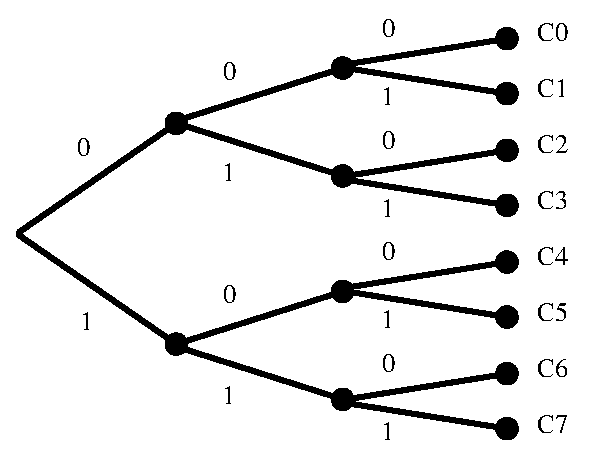
\epsfig{file=Figures/binarytree,width=7cm}
\end{psfrags}
\caption{This figure shows a binary tree with depth $L_c = 3$ and eight leaves.  The branches from every node correspond to zero or one.}
\label{figure:BinaryTree}
\end{center}
\end{figure}
Let $L_c = \max_{x \in \mathcal{X}} \ell_c (x)$ be the length of the longest codeword.
Code $c: \mathcal{X} \mapsto \mathcal{C}$ can be defined using a binary tree of depth $L_c$, where branches from every node correspond either to zero or one.
Each codeword consists of a unique path from the root to a leaf at depth $\ell_c(x)$, following its binary string expansion.
The prefix condition ensures that no codeword is a descendant of any other codeword in the binary tree.
For the codewords in the tree, let $S_x$ be the set of descendants that $c(x)$ would have in a full binary tree of depth $L_c$.
The sets $S_x$ are disjoint because of the prefix-free nature of the code, and $|S_x| = 2^{L_c - \ell_c(x)}$.
Since the total number of nodes at depth $L_c$ is $2^{L_c}$, we have
\begin{equation*}
\left| \bigcup_{x \in \mathcal{X}} S_x \right|
= \sum_{x \in \mathcal{X}} |S_x|
= \sum_{x \in \mathcal{X}} 2^{L_c - \ell_c(x)}
\leq 2^{L_c} .
\end{equation*}
By dividing both sides by $2^{L_c}$, we conclude that \eqref{equation:KraftInequality} holds.
That is, a binary prefix-free code $c$ over finite alphabet $\mathcal{X}$ satisfies the Kraft inequality.

Conversely, suppose that we have a code assignment such that \eqref{equation:KraftInequality} is satisfied.
Without loss of generality, we assume that the codeword lengths $\ell_c(x_i)$ are increasing in~$i$,
\begin{equation*}
\ell_c(x_1) \leq \ell_c(x_2) \leq \ell_c(x_3) \leq \cdots
\end{equation*}
We can construct a prefix code with matching codeword lengths by pruning subtrees from a  full binary tree of depth $L_c$.
First, choose any node from the full tree at depth $\ell_1$ and remove all of its descendants.
This removes $2^{L_c -\ell_1}$ leafs from the original binary tree.
Next, select any available node from the resulting tree at depth $\ell_2$, and remove all of its descendants.
This time, an additional $2^{L_c - \ell_2}$ leafs are taken away from the original binary tree.
Continue this procedure with the other codeword lengths.
After $m$ iterations, the total number of leafs removed from the original binary tree is equal to
\begin{equation*}
\sum_{i=1}^m 2^{L_c - \ell_i} = 2^{L_c} \sum_{i=1}^m 2^{-\ell_i} .
\end{equation*}
Since the Kraft inequality holds for the codeword length assignment, this implies that all the codewords can be placed at different positions on the binary graph.
Then, following the binary structure of the graph, the binary string of the codes can be inferred from the graph.
\end{proof}

\begin{example}[Code on a Tree]
Suppose that we intend to construct a prefix code for $\mathcal{X} = \{ x_1, \ldots, x_5 \}$, with code lengths
\begin{xalignat*}{3}
\ell_c(x_1) &= \ell_c(x_2) = 2 & \ell_c(x_3) &= \ell_c(x_4) = 3 & \ell_c(x_5) &= 2.
\end{xalignat*}
First, we check the Kraft inequality to make sure that such an assignment is feasible,
\begin{equation*}
\sum_{i = 1}^5 2^{-\ell_c(x_1)}
= \frac{1}{4} + \frac{1}{4} + \frac{1}{8} + \frac{1}{8} + \frac{1}{4} = 1 .
\end{equation*}
The inequality is fulfilled, we can therefore use a binary tree construction to design the desired instantaneous code.
The process is illustrated in Figure~\ref{figure:BinaryTreeCode}, and the resulting code is shown below.

\begin{center}
\begin{tabular}{|c|c|c|c|}
\hline
Source Symbol & Codeword & Source Symbol & Codeword \\
\hline
$x_1$ & 00 & $x_4$ & 101 \\
$x_2$ & 01 & $x_5$ & 11 \\
$x_3$ & 100 & & \\
\hline
\end{tabular}
\end{center}

Since the Kraft inequality is met with equality, we know that it is impossible to get a better code by shortening one of the codewords.
\begin{figure}[htbp]
\begin{center}
\begin{psfrags}
\psfrag{0}[c]{$0$}
\psfrag{1}[c]{$1$}
\psfrag{00}[l]{$00$}
\psfrag{01}[l]{$01$}
\psfrag{100}[l]{$100$}
\psfrag{101}[l]{$101$}
\psfrag{11}[l]{$11$}
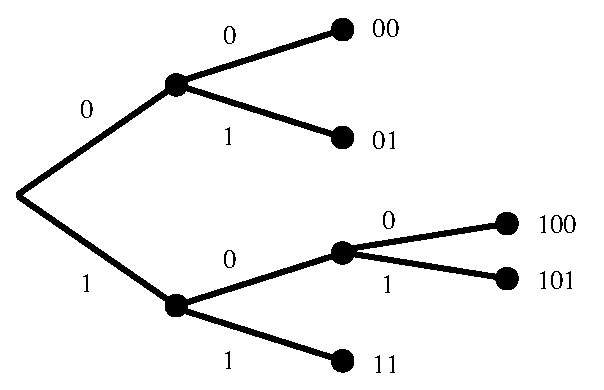
\epsfig{file=Figures/binarytreecode,width=7cm}
\end{psfrags}
\caption{Construction of a prefix code with a binary tree.}
\label{figure:BinaryTreeCode}
\end{center}
\end{figure}
\end{example}


\subsection{Entropy Bounds on Prefix-Free Codes}

Now that we know how to build instantaneous, we consider the problem of finding good prefix-free codes.
Recall from \eqref{equation:CodeRateCompression} that our objective is to find a prefix-free code with the smallest possible expected length.
As seen earlier, this codeword length assignment is subject to the Kraft inequality.
Putting these two requirements together, we can formulate the optimization problem as follows,
\begin{equation*}
\min_{\ell(x)} \sum_{x \in \mathcal{X}} p_X(x) \ell(x)
\quad \text{subject to} \quad
\sum_{x \in \mathcal{X}} 2^{- \ell(x)} \leq 1 .
\end{equation*}
We note that, for a code to exist, the function $\ell(x)$ must take values in the positive integers.
It turns out that this problem is difficult to solve.

To gain insight into the problem, we relax the integer constrain on $\ell(x)$.
This added flexibility will provide a lower bound on $\mathrm{E} [\ell(X)]$; having more choices can only lead to better results.
We use the method of Lagrange multipliers to solve the latter version of the problem.
The objective function, with Lagrange multiplier $\lambda$, becomes
\begin{equation*}
\sum_{x \in \mathcal{X}} p_X(x) \ell(x)
+ \lambda \left( \sum_{x \in \mathcal{X}} 2^{- \ell(x)} - 1 \right) .
\end{equation*}
Note that this function is twice differentiable in $\ell(x)$.
Taking a partial derivative with respect to $\ell(x)$ and setting it to zero, we get
\begin{equation*}
p_X(x) - \lambda \ln(2) 2^{- \ell(x)}  = 0 .
\end{equation*}
The optimal value for $\ell(x)$, which we denote by $\ell^{\star}(x)$, must therefore satisfy $2^{- \ell^{\star}(x)} = p_X(x) / (\lambda \ln (2))$.
Computing the derivative with respect to $\lambda$ yields
\begin{equation*}
\sum_{x \in \mathcal{X}} 2^{- \ell^{\star}(x)} = 1 ,
\end{equation*}
which in turn implies $\lambda = 1 / \ln (2)$.
Putting these results together, we gather that the optimal values for $\{ \ell(x) : x \in \mathcal{X} \}$ are given by
\begin{equation*}
\ell^{\star}(x) = - \log_2 (p_X(x))
\end{equation*}
for $x \in \mathcal{X}$.
Thus, by construction, we obtain
\begin{equation*}
\mathrm{E} [\ell_c(X)] \geq - \sum_{x \in \mathcal{X}} p_X(x) \log_2 (p_X(x))
= \mathrm{H}[X]
\end{equation*}
for any prefix-code~$c$.
In other words, the entropy is a lower bound on the expected length of any prefix-free code.

It is equally easy to obtain an upper bound on the expected length of an optimal prefix-free code.
Observe that $\lceil - \log_2 (p_X(x)) \rceil$ is an integer, with
\begin{equation*}
- \log_2 (p_X(x))
\leq \lceil - \log_2 (p_X(x)) \rceil
\leq - \log_2 (p_X(x)) + 1 .
\end{equation*}
The Kraft inequality asserts that we can build a code $c : \mathcal{X} \mapsto \mathcal{C}$ such that $\ell_c(x) = \lceil - \log_2 (p_X(x)) \rceil$, as
\begin{equation*}
\sum_{x \in \mathcal{X}} 2^{- \ell_c(x)}
\leq \sum_{x \in \mathcal{X}} 2^{- \ell^{\star}(x)} = 1 .
\end{equation*}
As such, there exists a code~$c$ such that
\begin{equation*}
\mathrm{E} [\ell_c(X)] \leq \mathrm{H}[X] + 1 .
\end{equation*}
We collect and formalize these important results in the form of a theorem.

\begin{theorem} \label{theorem:EntropyBoundsPrefixCodes}
Consider a discrete memoryless source $(\mathcal{X}, p_X(\cdot))$ over a finite alphabet.
If symbols are encoded individually using an optimal prefix-free code $c : \mathcal{X} \mapsto \mathcal{C}$, then the expected length of the codewords satisfies
\begin{equation*}
\mathrm{H}[X] \leq \mathrm{E} [\ell_c(X)] \leq \mathrm{H}[X] + 1 .
\end{equation*}
\end{theorem}


\subsection{Huffman Codes}

Theorem~\ref{theorem:EntropyBoundsPrefixCodes} identifies properties of an optimal prefix-code.
However, it does not provide an algorithmic methodology to design such a code.
This is addressed by the \defn{source coding}{Huffman code}, which provides an efficient variable-length code for lossless data compression.
Not too surprisingly, the underlying strategy in this scheme is to assign short strings of bits to likely symbols, and necessarily longer ones to less probable source outputs.
The encoding is specifically crafted so that the code table forms a prefix-free code.
Huffman codes are the most efficient compression mapping for individual source symbols.
The expected length of the compressed data achieved with this technique will be no greater than the expected message length of any other prefix-free code that operates on individual source symbols.

The insight behind Huffman coding is based on three properties of optimal prefix-codes.
Suppose that we wish to encode outputs from discrete memoryless source $(\mathcal{X}, p_X)$, and let $c^{\star} : \mathcal{X} \mapsto \mathcal{C}$ be an optimal prefix-code for this source.
If $p_X(x_1) > p_X(x_2)$, then $\ell_{c^{\star}}(x_1) \leq \ell_{c^{\star}}(x_2)$.
For any of the longest codewords, its sibling (the bit string that differs only in the last digit) must also be codeword; otherwise, the original codeword can be shortened by removing the last bit.
Finally, the code tree associated with an optimal code must be full.
A binary tree is \emph{full} if every node has either zero or two children.
Again, if this condition fails, then some codewords in the codebook can be shortened.

The Huffman algorithm creates a code by building a binary tree.
The algorithm proceeds as follows.
First, every source symbol $x$ is assigned to an individual node.
Then, the simple recursion outlined below is applied.
\begin{enumerate}
\item Sort the nodes in decreasing order of probabilities.
\item Merge the two least probable nodes into a single one, whose probability equals the sum of its constituents.
\item Arbitrarily assign zero or one to the branches emerging from this new node.
\item Repeat the previous three steps with the new collection of nodes and their corresponding probabilities until only one node remains.
\end{enumerate}
The Huffman encoding algorithm is best grasped through simple examples.

\begin{example}
Suppose that a discrete memoryless source $(\mathcal{X}, p_X)$ with alphabet $\mathcal{X} = \{ x_1, x_2, x_3 \}$ has probability mass function
\begin{equation*}
p_X(x) = \begin{cases} \frac{2}{3}, & x = x_1 \\
\frac{1}{6}, & x \in \{ x_2, x_3 \} . \end{cases}
\end{equation*}
We wish to obtain an optimal prefix-code for this source, and thus we apply the Huffman algorithm.
For the given source, code design proceeds as follows.

\begin{center}
\begin{tabular}{|c|c|c|c|c|}
\hline
Stage 3 & Stage 2 & Stage 1 & Symbol & Codeword \\
\hline
$\Pr \{ x_1, x_2, x_3 \} = 1$ & $\Pr \{ x_1 \} = \frac{2}{3}$
& $p_X (x_1) = \frac{2}{3}$ & $x_1$ & 0 \\
& $\Pr \{ x_2, x_3 \} = \frac{1}{3}$ & $p_X (x_2) = \frac{1}{6}$ & $x_2$ & 10 \\
& & $p_X (x_3) = \frac{1}{6}$ & $x_3$ & 11 \\
\hline
\end{tabular}
\end{center}

From this successive re-ordering of probabilities, we use a binary tree to build the actual code.
This is illustrated in Figure~\ref{figure:Huffman1}.
\begin{figure}[htbp]
\begin{center}
\begin{psfrags}
\psfrag{C1}[l]{$0$}
\psfrag{C2}[l]{$10$}
\psfrag{C3}[l]{$11$}
\psfrag{x1}[c]{$x_1$}
\psfrag{x2}[c]{$x_2$}
\psfrag{x3}[c]{$x_3$}
\psfrag{x23}[c]{$\{ x_2, x_3 \}$}
\psfrag{x123}[c]{$\{ x_1, x_2, x_3 \}$}
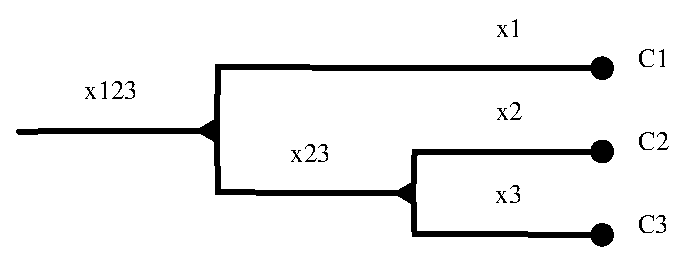
\epsfig{file=Figures/huffman1,width=68.718mm}
\end{psfrags}
\caption{A graphical representation for the construction of a simple Huffman code. The source alphabet in this case is $\mathcal{X} = \{x_1, x_2, x_3 \}$ and the probabilities of individual symbols are $\{ 2/3, 1/6, 1/6 \}$, respectively.}
\label{figure:Huffman1}
\end{center}
\end{figure}
\end{example}

\begin{example}
A source $(\mathcal{Y}, p_Y)$ generates four different symbols $\{ y_1, y_2, y_3, y_4 \}$ with probabilities $\{ 0.35, 0.25, 0.2, 0.2 \}$.
A binary tree is generated from right to left, by merging the two less probable symbols at every step.
Once this is complete, the code can then be form by assigning different bits to every pair of branches emerging from a node.
The table below shows the different stages of the iterative procedure where probabilities are first sorted in decreasing order, then the two least probable nodes are merged into a single one.

\begin{center}
\begin{tabular}{|c|c|c|c|}
\hline
Stage 4 & Stage 3 & Stage 2 & Stage 1 \\
\hline
$0.6 + 0.4 = 1$ & $0.35 + 0.25 = 0.6$ & $0.2 + 0.2 = 0.4$ & $p_X (x_1) = 0.35$ \\
& $0.4$ & $0.35$ & $p_X (x_2) = 0.25$ \\
& & $0.25$ & $p_X (x_3) = 0.2$ \\
& & & $p_X (x_4) = 0.2$ \\
\hline
\end{tabular}
\end{center}

The ensuing Huffman code is obtained by moving from left to right in the corresponding binary tree.
The binary tree and the resulting Huffman code are shown in Figure~\ref{figure:Huffman2}.

\begin{figure}[htbp]
\begin{center}
\begin{psfrags}
\psfrag{C1}[l]{$00$}
\psfrag{C2}[l]{$01$}
\psfrag{C3}[l]{$10$}
\psfrag{C4}[l]{$11$}
\psfrag{x1}[c]{$x_1$}
\psfrag{x2}[c]{$x_2$}
\psfrag{x3}[c]{$x_3$}
\psfrag{x4}[c]{$x_4$}
\epsfig{file=Figures/huffman2,width=87.791mm}
\end{psfrags}
\caption{This figure depicts a Huffman code construction for an alphabet of size four.}
\label{figure:Huffman2}
\end{center}
\end{figure}

\end{example}

Although Huffman coding is optimal for a symbol-by-symbol encoding with a known input probability mass function, it can be outperformed when these two conditions are not known.
For instance, if the input distribution $p_X(\cdot)$ is not known, then it must be inferred from the available data prior to applying Huffman coding.
Small errors in the estimated probability mass function can then lead to inefficiency, which in turn renders Huffman coding suboptimal.
We will soon see an encoding algorithm that does not require the input distribution $p_X(\cdot)$.
However, before we can present this algorithm, we need to consider the join encoding of source symbols.


\section{Joint Encoding of Source Symbols}

Under special circumstances, namely when the probability of every source symbol is an exponent base two, the expected length of a Huffman code is equal to the entropy of the source.
However, in many situations, this is not the case, and there exists a gap between the expected codeword length and the entropy of a source output.
An efficient way to encode data, where the expected number of coded bits per source symbol approaches the entropy, is to consider blocks of source symbols and to encode them jointly.
Although more complicated, this process leads to better performance and typically leads to expected message lengths that are shorter  than that of a symbol-by-symbol Huffman code.

Consider a sequence $X_1, X_2, \ldots$ of symbols at the output of a discrete memoryless source.
Instead of using a code that operates on individual symbols, we can design a more elaborate code that takes as input a group of $n$ symbols, $c: \mathcal{X}^n \mapsto \mathcal{C}$.
Since the outputs of a discrete memoryless source are independent and identically distributed random variables, we know from the additive property of the entropy that
\begin{equation*}
\mathrm{H}[X_1, \ldots, X_n ] = n \mathrm{H} [X] .
\end{equation*}
Then, by applying Theorem~\ref{theorem:EntropyBoundsPrefixCodes}, we get that an optimal prefix code, which operates on $\mathcal{X}^n$, yields
\begin{equation*}
n \mathrm{H}[X] \leq \mathrm{E} [ \ell_c (X_1, \ldots, X_n) ] \leq n \mathrm{H}[X] + 1.
\end{equation*}
Then, the expected message length per source output becomes
\begin{equation*}
\mathrm{H}[X] \leq \frac{ \mathrm{E} [ \ell_c (X_1, \ldots, X_n) ] }{n} \leq \mathrm{H}[X] + \frac{1}{n} .
\end{equation*}
Thus, the expected number of bits per symbol produced by a source can be made arbitrarily close to $\mathrm{H}[X]$ by jointly encoding strings of symbols.

\begin{example} \label{example:JointSourceCoding}
Let $(\mathcal{X}, p_X)$ be a binary discrete memoryless source, as described in Example~\ref{example:BinarySource}.
Furthermore, assume that Bernoulli parameter $p$ is equal to $\frac{1}{4}$.
Then, the entropy of the source can be calculated as
\begin{equation*}
\mathrm{H}[X] = - \frac{3}{4} \log_2 \left( \frac{3}{4} \right)
- \frac{1}{4} \log_2 \left( \frac{1}{4} \right)
\approx 0.811 .
\end{equation*}
Since there are only two source symbols, a code generated by the Huffman algorithm is the identity code, where a source output is represented by its binary value.
In this case, the expected codeword length is equal to one.

Suppose instead that two symbols are encoded at a time.
In this case, the possible inputs to the encoder are $\{ 00, 01, 10, 11 \}$, with respective probabilities $\left\{ \frac{9}{16}, \frac{3}{16}, \frac{3}{16}, \frac{1}{16} \right\}$.
The Huffman code specified by
\begin{center}
\begin{tabular}{|c|c|c|c|c|}
\hline
Symbol & Codeword \\
\hline
$00$ & 0 \\
$01$ & 10 \\
$10$ & 110 \\
$11$ & 111 \\
\hline
\end{tabular}
\end{center}
has an expected length of
\begin{equation*}
\mathrm{E} [\ell_c (X_1, X_2)] = 1 \cdot \frac{9}{16} + 2 \cdot \frac{3}{16}
+ 3 \cdot \frac{3}{16} + 3 \cdot \frac{1}{16}
= \frac{27}{16} . 
\end{equation*}
The expected message length per source output becomes
\begin{equation*}
\frac{\mathrm{E} [\ell_c (X_1, X_2)]}{2} = \frac{27}{32} \approx 0.844 ,
\end{equation*}
which is much closer to the entropy of individual source symbols.
Repeating this procedure with an Huffman code that takes three symbols as its input would lead to an expected codeword length per symbol of approximately $0.823$.
\end{example}

Example~\ref{example:JointSourceCoding} illustrates well how encoding several source symbol at a time can lead to a decrease in the expected codeword length per symbol.
The joint encoding of source symbols works even better for sources that are correlated over time.
Although we will not discuss the specifics of this scenario, it is informative to mention that joint source coding is instrumental in approaching the entropy rate of correlated sources.
This is especially important considering the fact that symbol-by-symbol encoding may perform very poorly for correlated sources.


\section{Fixed-Length Compression Codes}

In the previous section, the joint encoding of multiple source symbols was shown to perform well, with the average number of bits per symbol produced by a source approaching $\mathrm{H}[X]$.
Below, we explore how the joint encoding of symbols together with fixed-length codes can be used to produce good compression ratios.
Fixed-length compression codes have several advantages.
They are simple to encode and easy to decode, yielding unambiguous messages.
Furthermore, all fixed-length codes are prefix-free, and encoded symbols can therefore be recovered instantaneously.
However, fixed-length codes cannot be used to compress data by assigning short descriptions to most frequent symbols and longer descriptions to the less likely ones.
Data compression in fixed-length coding methods is only possible for large blocks of data, and any compression beyond the logarithm of the total number of possibilities comes with a finite, though perhaps small, probability of decoding failure.

The minimum number of binary strings in lossless fixed-length symbol-by-symbol encoding is $\left\lceil \log_2 ( | \mathcal{X} | ) \right\rceil$, where $| \mathcal{X} |$ is the size of the source alphabet and $\lceil \cdot \rceil$ is the ceiling function, which returns the smallest integer greater than or equal to its argument.
More generally, the minimum number of binary strings necessary to encode a group of $n$ symbols is $\left\lceil n \log_2 ( | \mathcal{X} | ) \right\rceil$.
This strategy alone, encoding multiple source symbols at a time, is not powerful enough to compress data using fixed-length codes.
To design effective fixed-length codes, two components are necessary.
First, we need to relax the assumption that the data compression scheme should be lossless, rather we allow a small probability of encoding failure.
In particular, we assume that the probability of encoding failure, where data cannot be decoded properly, is $\delta > 0$, where $\delta$ is implicitly very small.
The second ingredient to fixed-length compression is the asymptotic equipartition property, which we review next.


\subsection{Asymptotic Equipartition Property}

The \textbf{asymptotic equipartition property} (\defn{information theory}{AEP}) is a general property of the output samples of discrete memoryless sources.
This property implies that, given a very long sequence of $n$ source symbols, the probability that $(X_1, \ldots, X_n)$ belongs to a set of typical sample strings is almost one.
It takes a few steps to make this statement precise.

\begin{theorem} \label{theorem:WeakLawEntropy}
Let $(\mathcal{X}, p_X)$ be a discrete memoryless source, which produces a sequence of symbols $X_1, X_2, \ldots $
Furthermore, assume that the output alphabet $\mathcal{X}$ is finite.
The asymptotic equipartition probability asserts that
\begin{equation*}
\lim_{n \rightarrow \infty} - \frac{1}{n} \log_2 \left( p_{X^n} (X_1, \ldots X_n) \right)
= \mathrm{H} [X] .
\end{equation*}
\end{theorem}
\begin{proof}
We can proof this theorem through an application of the weak law of large numbers.
First, we observe that
\begin{equation*}
\begin{split}
\log_2 \left( p_{X^n} (X_1, \ldots X_n) \right)
&= \log_2 \left( \prod_{k=1}^n p_{X} (X_k) \right) \\
&= \sum_{k=1}^n \log_2 p_{X} (X_k) .
\end{split}
\end{equation*}
That is, $\log_2 \left( p_{X^n} (X_1, \ldots X_n) \right)$ is a sum of independent and identically distributed random variables, with bounded second moment.
It follows, by the law of large numbers, that
\begin{equation*}
- \frac{1}{n} \log_2 \left( p_{X^n} (X_1, \ldots X_n) \right)
\end{equation*}
converges in probability to $\mathrm{E} \left[ - \log_2 (p_X(X)) \right] = \mathrm{H}[X]$.
In particular, we have
\begin{equation*}
\Pr \left(
\left| \frac{- \log_2 \left( p_{X^n} (X_1, \ldots X_n) \right)}{n} - \mathrm{H}[X] \right|
\geq \epsilon \right)
\leq \frac{ \sigma^2}{n \epsilon^2}
\end{equation*}
where $\sigma^2$ is the variance of random variable $- \log_2 (p_X(X))$.
\end{proof}

Drawing intuition from the proof of Theorem~\ref{theorem:WeakLawEntropy}, we define the \defn{information theory}{typical set} $T_{\epsilon}^{(n)}$ as
\begin{equation*}
T_{\epsilon}^{(n)}
= \left\{ \mathbf{x} \in \mathcal{X}^n :
\left| \frac{- \log_2 \left( p_{X^n} (\mathbf{x}) \right)}{n} - \mathrm{H}[X] \right|
< \epsilon \right\} .
\end{equation*}
The probability that the first $n$ source symbols belongs to the typical set $T_{\epsilon}^{(n)}$ is bounded below by
\begin{equation} \label{equation:ProbabilityTypicalSet}
\Pr \left( (X_1, \ldots, X_n) \in T_{\epsilon}^{(n)} \right) \geq 1 - \frac{\sigma^2}{n \epsilon^2} .
\end{equation}
Thus, as $n$ increases, the probability that the source produces a typical sequence approaches one.
We note that an equivalent definition of typical set is
\begin{equation*}
T_{\epsilon}^{(n)}
= \left\{ \mathbf{x} \in \mathcal{X}^n :
2^{- n (\mathrm{H}[X] + \epsilon)} < p_{X^n} (\mathbf{x})
< 2^{- n (\mathrm{H}[X] - \epsilon)} \right\} .
\end{equation*}
Using the second definition of $T_{\epsilon}^{(n)}$, we can bound the number of elements contained in a typical set.
First, recall that the sum of the probability of disjoint events cannot exceed one.
As a consequence, the number of elements in $T_{\epsilon}^{(n)}$ is bounded by
\begin{equation*}
\left| T_{\epsilon}^{(n)} \right| < 2^{n (\mathrm{H}[X] + \epsilon)} .
\end{equation*}
Similarly, using \eqref{equation:ProbabilityTypicalSet} and the second definition of $T_{\epsilon}^{(n)}$, we get
\begin{equation*}
\left| T_{\epsilon}^{(n)} \right| > \left( 1 - \frac{\sigma^2}{n \epsilon^2} \right)
2^{n (\mathrm{H}[X] - \epsilon)} .
\end{equation*}
We collect these results in the following theorem.

\begin{theorem}[Asymptotic Equipartition Property] \label{theorem:AEP}
Let $(\mathcal{X}, p_X)$ be a discrete memoryless source with finite alphabet $\mathcal{X}$ and output sequence $X_1, X_2, \ldots$, each with entropy $\mathrm{H}[X]$.
For any $\delta > 0$ and all $n$ sufficiently large, we have
\begin{equation*}
\Pr \left( (X_1, \ldots, X_n) \in T_{\epsilon}^{(n)} \right) \geq 1 - \delta
\end{equation*}
and the size of the typical set $T_{\epsilon}^{(n)}$ is bounded by
\begin{equation*}
(1 - \delta) 2^{n (\mathrm{H}[X] - \epsilon)} <
\left| T_{\epsilon}^{(n)} \right| < 2^{n (\mathrm{H}[X] + \epsilon)} .
\end{equation*}
\end{theorem}

The intuition behind the asymptotic equipartition property is that a compression scheme can focus on encoding only the symbol strings that belong to $T_{\epsilon}^{(n)}$.
Under such a strategy, at most $\lceil n (\mathrm{H}[X] + \epsilon) \rceil$ codewords are needed.
Although not lossless, this fixed-length coding scheme results in a decoding failure with a probability no greater than $\delta$.

\begin{theorem}[Source Coding Theorem]
Let $(\mathcal{X}, p_X)$ be a discrete memoryless source with finite alphabet $\mathcal{X}$ and entropy $\mathrm{H}[X]$.
For any $\delta > 0$, $\epsilon > 0$ and $n$ sufficiently large, there exists a fixed-length compression scheme such that the probability of failure is less than $\delta$ and the expected number of bits per symbol is
\begin{equation*}
\frac{\mathrm{E} [\ell_c(X_1, \ldots, X_n)]}{n} \leq \mathrm{H}[X] + \epsilon + \frac{1}{n} .
\end{equation*}
\end{theorem}


\section{Universal Source-Coding Algorithms}

Huffman coding has two important drawbacks.
First, the source statistics are used to design a Huffman code.
If one only has access to the source outputs, the design procedure requires two passes through the data, one to estimate the statistics of the source, and a second one for encoding.
To overcome this, one can use adaptive Huffman codes where the code is updated dynamically to match the statistics of the sequence as it is observed.
This is a problem because
The second problem is that one must jointly encode multiple symbols to take advantage of source memory and reduce length rounding loss.
In this case, one finds that the complexity increases exponentially with the number of symbols that are encoded together.
To provide a partial solution to these drawbacks, we study an example of a universal source-coding algorithm, namely the Lempel-Ziv algorithm.
This type of \defn{source coding}{universal data compression} is the basis for standard file compression algorithms (e.g., winzip, gzip).

The basic idea behind the \defn{source coding}{Lempel-Ziv algorithm} is to parse the input sequence into non-overlapping strings of different lengths while constructing a dictionary of the strings seen thus far.
There are many versions of this algorithm and we discuss the variant known as LZ78 that was described in a 1978 paper by Lempel and Ziv.
The encoding algorithm works as follows.
First, initialize the dictionary to contain all strings of length one and set the input pointer to the beginning of the string.
Then, apply the following iterative procedure.
\begin{enumerate}
\item Starting at the input pointer, find the longest substring $w$ that is already in the dictionary.
\item Concatenate $w$ with the next symbol $y$ in the string and add $wy$ to the first empty location in the dictionary.
\item Encode the pair by sending the dictionary index of $w$ and the value of $y$.
\item Set the input pointer to the symbol after $y$.
\end{enumerate}
There are a number of practical variants of this algorithm that improve performance and/or reduce the implementation complexity.

Decompression works in the reverse fashion.
Each received index and symbol can be immediately decoded and used to build a copy of the dictionary at the receiver.
In this fashion, one can resolve the input without ambiguity.

\begin{example}
Suppose that we are to use a Lempel-Ziv algorithm with dictionary size $2^3 = 8$.
The dictionary is initialized to contain $0$ and $1$ in the first two positions.
Then, the source sequence is sequentially parsed into strings that have not appeared so far.
For example, 
\begin{equation*}
10110101000101 \ldots \rightarrow 10,11,01,010,00,101 \ldots
\end{equation*}
The dictionary table at this point has eight elements.

\begin{center}
\begin{tabular}{|c|c|c|c|}
\hline
Index & Dictionary String & Encoded Index & Added Bit \\
\hline
000 & 0 & N/A & N/A \\
001 & 1 & N/A & N/A \\
010 & 10 & 001 & 0 \\
011 & 11 & 001 & 1 \\
100 & 01 & 000 & 1 \\
101 & 010 & 100 & 0 \\
110 & 00 & 000 & 0 \\
111 & 101 & 010 & 1 \\
\hline
\end{tabular}
\end{center}

Each phrase (the bit string contained between two commas) is coded by giving the location of its prefix in the dictionary table, and the value of the additional bit.
This results in the coded sequence
\begin{equation*}
10,11,01,010,00,101 \rightarrow (001, 0)(001, 1)(000, 1)(100, 0)(000, 0)(010, 1),
\end{equation*}
where the first number of each pair gives the index of the prefix in the table and the second number gives the last bit of the new phrase. 
When applied to sequences generated by any stationary ergodic source, the Lempel-Ziv coding algorithm asymptotically achieves the optimal encoding rate (known as the entropy rate).
\end{example}

Most readers will notice that this algorithm, as stated, requires prior knowledge of the total number of phrases in the dictionary.
In fact, this problem can be solved easily and the solution actually requires fewer transmitted bits.
The key point is that both the transmitter and receiver know the number of phrases currently in the dictionary.
Let $M$ be the current number of phrases in the dictionary.
Then, the transmitter can be simply send the $\lceil \log_2 M \rceil$ least significant bits of the index.
Since the receiver also knows $M$, there will be no confusion.
In this case, the encoded sequence will be
\begin{equation*}
10,11,01,010,00,101 \rightarrow (1, 0)(01, 1)(00, 1)(100, 0)(000, 0)(010, 1).
\end{equation*}


\chapter{Discrete-Time Communication}
\label{chapter:DiscreteTimeComm}

Most digital communications systems operate by converting digital data into continuous waveforms that can be conveyed through some physical medium to a receiver.
For example, digital communication through wires (e.g., Ethernet or USB) is based on moving electrons back and forth in the wire.
In contrast, underwater wireless communication uses acoustic transmission through the water.
While radio communication relies on the propagation of electromagnetic waves through air.

The process by which a string of bits is converted into a waveform suitable for transmission is known as \defn{communication}{modulation}.
The reverse operation, called \defn{communication}{demodulation}, is performed at the destination and involves extracting the information symbols from the received signal.
The mapping between the transmitted waveform and the received waveform is known as the \defn{communication}{channel}.

Precise models of the physical channel can be very complicated and many of the key ideas in digital communication do not depend on the exact details.
For this reason, one can model and design communication systems based a simplified model that separates the communication problem from the physical models.
In this chapter, we develop some of basic concepts in digital communications using this simplified model.
The goal is to build some intuition about how things work without getting lost in the mathematical details.

\section{A Simple Channel Model}

\begin{figure}
\begin{center}
\scalebox{0.8}
{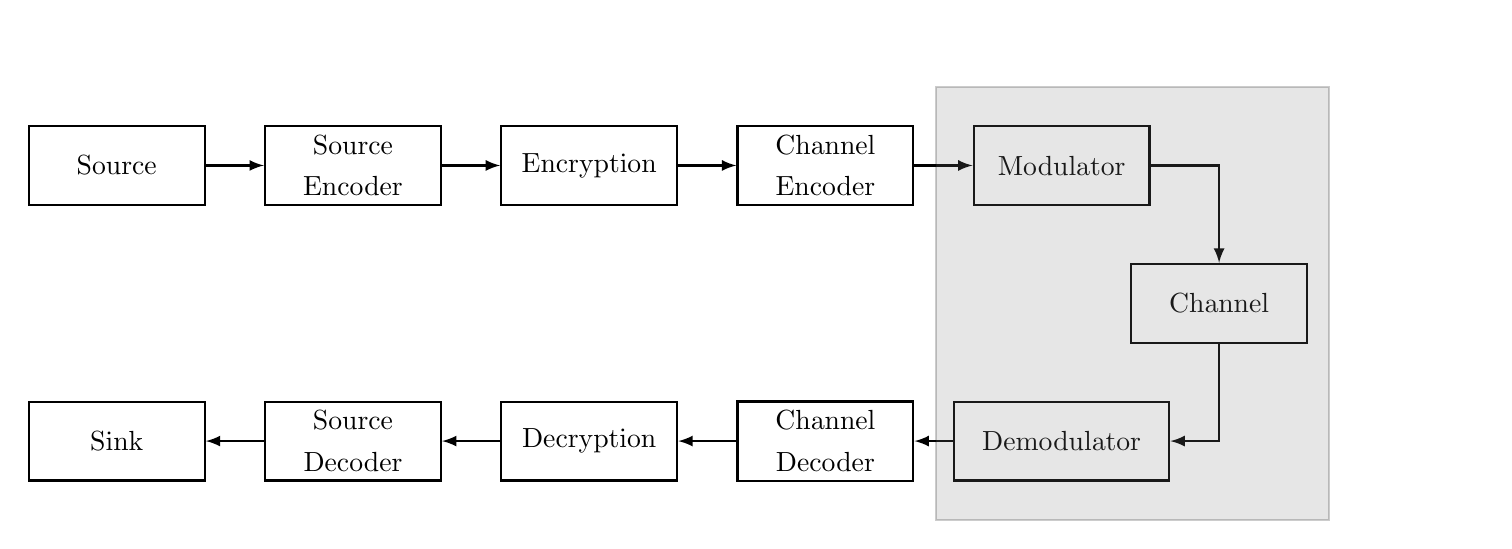
\begin{tikzpicture}[thick]
  \tikzstyle{every node}=[draw,text centered,text width=2cm,minimum height=1cm,shape=rectangle];
    \path (0,0) node (a) {Source}
          (0,1.25) node [draw=none] (aa) {}
          (3,0) node (b) {Source Encoder}
          (3,1.25) node [draw=none] (bb) {}
          (6,0) node (c) {Encryption}
          (6,1.25) node [draw=none] (cc) {}
          (9,0) node (d) {Channel Encoder}
          (9,1.25) node [draw=none] (dd) {}
          (12,0) node (e) {Modulator}
          (14,-1.75) node (f) {Channel}
          (16.25,-1.75) node [draw=none] (ff) {}
          (12,-3.5) node[text width=2.5cm] (g) {Demodulator}
          (9,-3.5) node (h) {Channel Decoder}
          (6,-3.5) node (i) {Decryption}
          (3,-3.5) node (j) {Source Decoder}
          (0,-3.5) node (k) {Sink};

    \draw[-latex] (a) -- (b);
    \draw[-latex] (b) -- (c);
    \draw[-latex] (c) -- (d);
    \draw[-latex] (d) -- (e);
    \draw[-latex] (e) -| (f);
    \draw[-latex] (f) |- (g);
    \draw[-latex] (g) -- (h);
    \draw[-latex] (h) -- (i);
    \draw[-latex] (i) -- (j);
    \draw[-latex] (j) -- (k);

    \filldraw[fill=gray,opacity=0.20] (10.4,1) rectangle (15.4,-4.5);
%    \draw (12.7,-5) node [draw=none,text width=10cm] (gg) {Discrete-Time Equivalent Channel};

\end{tikzpicture}}
\end{center}
\vspace{-4mm}
\caption{The block diagram of a digital communication system where the blocks comprising the discrete-time channel are shaded.}
\end{figure}

In this section, we introduce the \defn{communication}{discrete-time channel model} for digital communication systems.
We will see later that, for some communication systems, this model is exactly equivalent to the more complicated waveform model.
The first channel model we discuss is where the $n$th output of the channel, $Y_n$, is equal to the $n$th input to the channel, $x_n$, corrupted by an additive noise term $Z_n$ so that
\[ Y_n = x_n + Z_n. \]
For this model, it is typical to assume that the noise sequence $Z_1, Z_2, \ldots$ consists of independent identically distributed (i.i.d.) zero-mean Gaussian random variables with variance $\sigma^2$.
This implies that each $Y_n$ is a Gaussian random variable with mean $x_n$ and variance $\sigma^2$, so that
\[ f_{Y_n}(y_n) = \frac{1}{\sqrt{2\pi \sigma^2}} e^{-(y_n - x_n)^2 / (2\sigma^2)}.\]
This model is commonly referred to as discrete-time communication in \defn{communication}{additive white Gaussian noise} (AWGN) noise.

As an example, consider a system where the transmitter sets the voltage on end of a wire and the receiver measures the voltage on the other end of the wire.
It turns out that the thermal agitation of electrons causes voltage fluctuations known as Johnson noise.
So, the receiver ends up measuring the transmitted voltage corrupted by noise fluctuations.
In fact, Johnson noise is quite well approximated by AWGN.
So, the simple model described above already gives a relatively accurate picture of reality.

\section{A Simple Modulation Scheme}

Once a channel model has been defined, the next step is choosing how to transmit digital data through the channel.
A common approach is to choose a small set $\mathcal{U}$ of information symbols and represent each one by a distinct channel input in the set $\mathcal{X}$.
This is the discrete-time model of a scheme known as \defn{communication}{pulse-amplitude modulation} (PAM).
Let $u_n \in \mathcal{U}$ be the information symbol transmitted during the $n$th time interval and $x_n = M(u_n)$ be the $n$th input to the channel, where $M: \mathcal{U} \rightarrow \mathcal{X}$ is called the symbol mapping function.
For example, one can transmit binary information symbols by mapping ``0" to $+1$V and ``1" to $-1$V; mathematically, this is done by choosing $\mathcal{U}=\{0,1\}$, $\mathcal{X}=\{-1,1\}$, and $M(u) = 1-2u$.
This particular type of PAM is called \defn{communication}{binary phase-shift keying} (BPSK) or 2-PAM.

Suppose a BPSK signal is transmitted through our discrete-time AWGN channel model.
The detector must measure the voltage and decide whether a 0 or 1 one was transmitted.
A natural choice is to define a decoder function that associates positive voltages with 0 and negative voltages with 1.
Let $\hat{U}_n = D(Y_n)$ be the output of the detector function
\[ D(y) = \begin{cases} 0 & \text{if }y\geq0 \\ 1 & \text{if }y<0 \end{cases}. \]
This detector is optimal if 0's and 1's are transmitted with equal probability.

One of the main challenges in communication systems is providing reliable data transmission.
In this example, the noise variance $\sigma^2$ is proportional to the power of the thermal noise in the wire.
Notice that, if a 1 is transmitted, the detector described above will make an incorrect decision with probability
\[ \Pr \left( Y_n \geq 0 | x_n = 1 \right) = \Pr \left( Z_n \geq 1 \right) = \int_{1}^{\infty}  \frac{1}{\sqrt{2\pi \sigma^2}} e^{-y^2 / (2\sigma^2)} dy = Q\left( \frac{1}{\sigma} \right).\]
This probability can be reduced by increasing the transmitted voltage, which increases the power dissipated due to resistive losses, or by reducing the thermal noise.
For this reason, receivers used for large satellite dish receivers often use liquid nitrogen to cool the first-stage amplifier to reduce this thermal noise.
On the other hand, the maximum transmitted power is typically limited by physical constraints (e.g., the wire thickness) or FCC regulations.

\begin{figure}[t]
\begin{center}
\scalebox{0.75}
{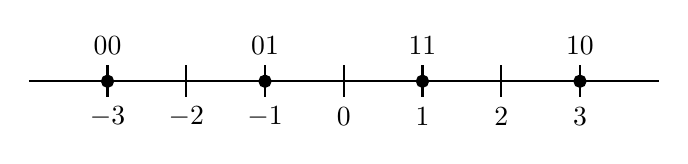
\begin{tikzpicture}[thick]

  \draw (-4,0) -- (4,0);

  \foreach \x in {-3,-2,...,3}
  {
    \draw (\x,-0.20) -- (\x,0.20);
    \draw (\x,-0.45) node {$\x$};
  }

  \foreach \x/\y in {-3/00,-1/01,1/11,3/10}
  {
    \draw (\x,+0.45) node {$\y$};
    \filldraw (\x,0) circle (2pt);
  }

\end{tikzpicture}}
\end{center}
\vspace{-6mm}
\caption{The symbol set $\mathcal{X}$ for 4-PAM with gray coded binary labels.}
\end{figure}

To send more information per channel use, one can use larger sets of PAM symbols.
For example, 4-PAM uses the 4 symbols $\mathcal{X}=\{ -3,-1,1,3 \}$ while 8-PAM uses the 8 symbols $\mathcal{X}=\{-7,-5,-3,-1,1,3,5,7\}$.
Notice that these two sets of symbols are centered around 0 to minimize the transmitted energy.

The mapping function $M(\cdot)$ determines the information symbol associated with each channel input value.
In general, sets of input values with $2^m$ elements are associated with binary strings.
There are still some choices to be made, however, because one can map the 4-PAM symbol set to binary strings in either the standard binary order $\{00,01,10,11\}$ or with a Gray code $\{00,01,11,10\}$.

For the 4-PAM symbol set with the mapping function $M(\cdot)$ that maps $\{00,01,10,11\}$ (in order) to $\{-3,-1,1,3\}$, the natural decision function is
\[ D(y) = \begin{cases}
00 & \text{if }y < -2 \\
01 & \text{if }-2 \leq y<0 \\
10 & \text{if }0 \leq y< 2 \\
11 & \text{if }y \geq 2
\end{cases}. \]

\section{Quadrature Amplitude Modulation}

In most communication systems, the baseband waveform is modulated onto a high-frequency carrier to enable better propagation.
This is because low-frequency signals often do not propagate well through physical media.
While this process will be discussed later in more detail, the following key detail affects the discrete-time model.
High frequency modulation allows two independent signals to be modulated onto the same carrier frequency; one onto the sine wave and the other onto the cosine wave.
This allows one to treat the transmitted value $x_n$ and received value $Y_n$ as points in 2-dimensional space.
The set $\mathcal{X}$ of possible transmitted points in 2-dimensional space in called the \defn{communication}{symbol constellation}.

\begin{figure}
\begin{center}
\scalebox{0.5}
{\begin{tikzpicture}[thick]

  \draw (-4,0) -- (4,0);
  \draw (0,-4) -- (0,4);

  \foreach \x in {-3,-2,...,3}
    \draw (\x,-0.20) -- (\x,0.20);

  \foreach \y in {-3,-2,...,3}
    \draw (-0.20,\y) -- (0.20,\y);

  \foreach \x in {-3,-1,1,3}
  \foreach \y in {-3,-1,1,3}
  {
    \filldraw (\x,\y) circle (2pt);
  }

\end{tikzpicture}}
\hspace{5mm}
\scalebox{0.5}
{\begin{tikzpicture}[thick]

  \draw (-4,0) -- (4,0);
  \draw (0,-4) -- (0,4);

  \foreach \x in {-3,3}
    \draw (\x,-0.20) -- (\x,0.20);

  \foreach \y in {-3,3}
    \draw (-0.20,\y) -- (0.20,\y);

  \foreach \x/\y in {3/0,2.12/2.12,0/3,-2.12/2.12,-3/0,-2.12/-2.12,0/-3,2.12/-2.12}
  {
    \filldraw (\x,\y) circle (2pt);
  }

\end{tikzpicture}}
\end{center}
\caption{The symbol constellations $\mathcal{X}$ for 16-QAM (left) and 8-PSK (right).}
\end{figure}

For mathematical convenience, points in these two-dimensional symbol constellations are represented by complex numbers.
The set of complex numbers is $\mathbb{C}$ and the constellation is a subset $\mathcal{X}\subset\mathbb{C}$.
Likewise, the transmitted symbol is $x_n \in \mathbb{C}$ and the received value is $Y_n \in \mathbb{C}$.
The noise term $Z_n$ now consists of two i.i.d. Gaussian random variables (one in each direction).
The probabilistic observation model is formed by treating the real and imaginary parts separately, and is given by
\begin{align*}
f_{Y^{(r)}_n,Y^{(i)}_n}(y^{(r)}_n,y^{(i)}_n) & =
\left( \frac{1}{\sqrt{2\pi \sigma^2}} e^{-\left(y^{(r)}_n - x^{(r)}_n\right)^2 / (2\sigma^2)} \right)
\left( \frac{1}{\sqrt{2\pi \sigma^2}} e^{-\left(y^{(i)}_n - x^{(i)}_n\right)^2 / (2\sigma^2)} \right) \\
& =  \frac{1}{2\pi \sigma^2} e^{-\left|y_n - x_n\right|^2 / (2\sigma^2)}.
\end{align*}
Therefore, the probability of receiving a $y_n$ value is simply a function of its Euclidean distance $\left| y_n - x_n \right|^2$ from the actual transmitted symbol.
This leads to a nice geometric characterization of the optimal decision regions for the detector.

The \defn{communication}{signal-to-noise ratio} (SNR) of a communication system is typically denoted by $E_s / N_0$ where $E_s$ is the average \textbf{energy per channel input symbol} and $N_0$ is the \defn{communication}{noise spectral density}.
For equiprobable signaling, one finds that
\[ E_s = \frac{1}{|\mathcal{X}|} \sum_{x\in \mathcal{X}} |x|^2. \]
The noise spectral density measures how much the AWGN is affects the channel and later we will see that $N_0 = 2 \sigma^2$ for our discrete-time model.

Constellations are typically defined by first choosing the set of channel input values $\mathcal{X}$, and then choosing the mapping function $M:\mathcal{U} \rightarrow \mathcal{X}$.
This second step is called \textbf{labeling} the constellation.
While the labeling does not affect the symbol error rate of the system, it generally does affect the bit error rate.
Therefore, one can optimize the mapping function for a particular application.

Constellations can be chosen and optimized for a variety of reasons.
Still, there are a few very common choices:
\begin{itemize}
\item $M$-ary PAM ($M$-PAM) is $M$ points equally spaced along a line or
\[ \mathcal{X} = \left\{ 2a-(M-1) \, \big| \, a \in \{0,1,\ldots,M-1\} \right\} \subset \mathbb{C}. \]

\item $M^2$-ary QAM ($M^2$-QAM) is an $M$ by $M$ square grid of points or
\[ \mathcal{X} = \left\{ \left(2a-(M-1)\right)+ \left(2b-(M-1)\right)i \, \big| \, a,b \in \{0,1,\ldots,M-1\} \right\} \subset \mathbb{C}. \]

\item $M$-ary PSK ($M$-PSK) is $M$ points equally spaced around a circle or
\[ \mathcal{X} = \left\{ e^{2\pi i k/M} \, \big| \, k \in \{0,1,\ldots,M-1\} \right\} \subset \mathbb{C}. \]
\end{itemize}

\begin{example}
The standard QAM constellation with 16 points (known as 16-QAM) is given by
\[ \mathcal{X} = \left\{ a+bi \, \big| \, a,b \in \{-3,-1,1,3\} \right\} \subset \mathbb{C}. \]
The average energy of this constellation is given by
\[ E_s = \frac{1}{16} \sum_{a,b\in \{-3,-1,1,3\}} (a^2 + b^2) = \frac{8}{16}  \sum_{a\in \{-3,-1,1,3\}} a^2 = 10.\]
\end{example}

\section{Optimal Symbol Detection}
\index{hypothesis testing}

In this section, we consider the problem of designing a symbol detector that minimizes the probability of error.
This is known as an \defn{communication}{optimal detection} problem and has an elegant solution that is related to the classical problem of \textbf{hypothesis testing} in statistics.

\subsection{Hypothesis Testing}

Sir Ronald Fisher, one of the founders of statistical decision theory, was at a tea party when Ms. Bristol mentioned that she preferred tea poured into milk over milk poured into tea.
Fisher commented that surely she could not tell the difference, but his colleague William Roach suggested that they design an experiment.
At that point, they prepared eight cups of tea: four milk-into-tea and four tea-into-milk.
The cups were presented in a random order and she correctly identified enough (all eight cups by some accounts) to prove her point.

Adding math to this requires that one defines carefully ``can tell the difference", but this is not a big problem because, for example, one can use the hypothesis $H_0=$``her success rate is more than three out of four".
There are more subtle issues, however, such as the meaning of passing the test.
While Ms. Bristol may do this by luck, this is also easy to analyze with calculations.
What is more problematic is understanding all the other hypotheses that can lead to the same observation.
For example, she may pass by cheating but still be unable to distinguish between the two drinks.
If this hypothesis is not explicitly considered, one can come to an incorrect conclusion.

For this reason, any scientific test of a hypothesis can only \emph{disprove} that hypothesis.
If Ms. Bristol cannot get 75\% correct in a larger test, then we can be reasonably confident that ``her ability to distinguish does not meet our threshold of three times out of four".
This is an example of a \defn{hypothesis testing}{null hypothesis} statistical test where the hypothesis can only disproven reliably.
Adding some math to this example shows that
\[ \Pr (\text{she identifies all cups correctly} | H_0 \text{ is false}) \leq (3/4)^8 \approx 0.10. \]
Therefore, the observation does not support the falsification of $H_0$.
Not much more can be concluded from this experiment.

\subsection{Multiple Hypothesis Testing}

Hypothesis testing in communication theory often has the luxury that one of the hypotheses must be true.
This leads to the more well-defined problem of \defn{hypothesis testing}{multiple hypothesis testing}.
Instead of testing a single hypothesis to see if it is false, one can compare multiple hypothesis to see which is most supported by the observation.

Let $H_0,H_1,\ldots,H_{m-1}$ be $m$ different hypotheses that affect a random observation $Y$.
The probability of a hypothesis before the observation, $\Pr(H_i)$, is called the \defn{hypothesis testing}{a priori probability}.
For each hypothesis, the connection with $Y$ is defined by the \defn{hypothesis testing}{observation probability} $\Pr (Y=y \, | \, H_i)$.

The goal is to choose a decision function $D(y)$ which, for any observation, minimizes the decision error probability.
Of course, this is equivalent to maximizing the probability that the decision is correct.
Notice that, if $Y=y$, then the probability that hypothesis $H_i$ is correct is given by its \defn{hypothesis testing}{a posteriori probability} $\Pr (H_i \, | \, Y=y )$.
Therefore, one finds that the optimal choice is the \defn{hypothesis testing}{maximum a posteriori} \textbf{probability} (MAP) decision rule 
\[ D(y) = \underset{i\in\{0,\ldots,m-1\}}{\mathrm{arg\,max}} \Pr( H_i \, |  \, Y=y). \]

In practice, these probabilities can be computed with Bayes' rule using only the a priori probabilities and observation probabilities.
This gives
\[ \Pr \left(H_i | Y=y \right) =
\frac{\Pr(H_i) \Pr (Y=y | H_i) }{\sum_{j=0}^{m-1} \Pr(H_j) \Pr (Y=y | H_j)}. \]
Since the denominator of this expression is the same for all $i$, the MAP rule can be simplified to
\[ D(y) = \underset{i\in\{0,\ldots,m-1\}}{\mathrm{arg\,max}} \Pr(H_i) \Pr (Y=y | H_i). \]

\begin{example}
Consider a system which transmits BPSK over an AWGN channel.
Let $H_0$ be the hypothesis that a zero (i.e., $+1$) was sent and $H_1$ be the hypothesis that a one (i.e., $-1$) was sent.
For binary hypothesis problems, the MAP decision rule can be written as
\[ \Pr (H_0) \Pr (Y=y | H_0) \underset{H_1}{\overset{H_0}{\gtrless}}  \Pr (H_0) \Pr (Y=y | H_0, \]
where this notation implies that one should pick $H_0$ if the LHS is greater than the RHS and $H_1$ otherwise.
If $\Pr(H_0) = 1-p$ and $\Pr (H_1) = p$, then one can substitute formulae to rewrite this as
\[ (1-p)  \frac{1}{\sqrt{2\pi \sigma^2}} e^{-(y-1)^2 / (2\sigma^2)} \underset{H_1}{\overset{H_0}{\gtrless}}  p \frac{1}{\sqrt{2\pi \sigma^2}} e^{-(y+1)^2 / (2\sigma^2)}.\]
After a little algebra, taking the logarithm of both sides simplifies this to 
\[ y \underset{H_1}{\overset{H_0}{\gtrless}} \frac{\sigma^2}{2}  \ln \frac{p}{1-p}.\]
\end{example}

Another popular rule is the \defn{hypothesis testing}{maximum likelihood} (ML) decision rule
\[ D(y) = \underset{i\in\{0,\ldots,m-1\}}{\mathrm{arg\,max}} \Pr (Y=y | H_i), \]
which ignores the a priori probability.
When all the hypotheses have the same a priori probability, these two rules are identical.
In communication systems, this is often the case.

\begin{example}
Consider a system which transmits 4-PAM (i.e, $\mathcal{X}=\{-3,-1,1,3\}$) over an AWGN channel.
If all channel inputs are equiprobable, then the optimum detector is
\begin{align*}
D(y)
& =  \underset{x\in\{-3,-1,1,3\}}{\mathrm{arg\,max}} \left( \frac{1}{\sqrt{2\pi \sigma^2}} e^{-(y-x)^2 / (2\sigma^2)} \right) \\
& =  \underset{x\in\{-3,-1,1,3\}}{\mathrm{arg\,max}} \left(-\frac{1}{2}\ln(2\pi \sigma^2) - \frac{1}{2\sigma^2} (y-x)^2 \right) \\
& =  \underset{x\in\{-3,-1,1,3\}}{\mathrm{arg\,min}} (y-x)^2. 
\end{align*}
Therefore, the optimum detector chooses the constellation point closest to the channel observation.
Moreover, this statement remains true for any signal constellation with equiprobable signalling and AWGN.
\end{example}


\chapter{Fourier Analysis and Sampling}
\label{chapter:FourierAnalysisSampling}

\emph{Fourier analysis} refers to a collection of tools that can be applied to express a function in terms of complex sinusoids, called basis elements, of different frequencies.
The result of the decomposition is the amplitude and the phase to be imparted to each basis element in the reconstruction.
This decomposition is termed the \emph{frequency domain representation} of the original signal.

Fourier analysis is extremely useful in engineering, with a myriad of applications.
Part of its appeal lies in the fact that basis elements are characteristic functions of linear time-invariant systems.
This property, which may seem nebulous at this point, is instrumental in solving many challenging problems, and makes Fourier analysis a powerful methodology for the design of communication systems.
We assume that the reader is familiar with basic Fourier analysis, and only review details that are pertinent to our treatment of communication systems.
This is not intended to be a comprehensive treatment of harmonic analysis.


\section{Fourier Series}
\label{section:FourierSeries}

Fourier series can be employed to express, as weighted sums of sinusoidal components, either periodic functions or functions that are time-limited.
Suppose that $s(t)$ is a function that is nonzero only for $-\frac{T}{2} \leq t \leq \frac{T}{2}$, and is square integrable
\begin{equation*}
\| s(t) \|^2 = \int_{\mathbb{R}} |s(t)|^2 dt
= \int_{-\frac{T}{2}}^{\frac{T}{2}} |s(t)|^2 dt < \infty .
\end{equation*}
Then $s(t)$ possesses a \emph{Fourier series representation}, which is defined by
\begin{equation} \label{equation:FourierSeries1}
s(t) = \begin{cases} \sum_{k=-\infty}^{\infty}
\hat{s}_k e^{2 \pi i \frac{k}{T} t}, & |t| \leq \frac{T}{2} \\
0, & \text{otherwise} \end{cases}
\end{equation}
where the Fourier series coefficients $\{ \hat{s}_k : k \in \mathbb{Z} \}$ are given by
\begin{equation*}
\hat{s}_k = \frac{1}{T} \int_{-\frac{T}{2}}^{\frac{T}{2}}
s(t) e^{-2 \pi i \frac{k}{T} t} dt .
\end{equation*}
We can use the standard rectangular function $\mathrm{rect}(\cdot)$, defined by
\begin{equation} \label{equation:RectangularFunction}
\mathrm{rect} (t) = \begin{cases} 1, & |t| < 0.5 \\
0, & \text{otherwise} \end{cases}
\end{equation}
to simplify \eqref{equation:FourierSeries1}, and rewrite the Fourier representation of $s(t)$ as
\begin{equation} \label{equation:FourierSeries2}
s(t) = \sum_{k=-\infty}^{\infty}
\hat{s}_k e^{2 \pi i \frac{k}{T} t}
\mathrm{rect} \left( \frac{t}{T} \right) .
\end{equation}
From a vector space perspective, \eqref{equation:FourierSeries2} asserts that $s(t)$ can be expressed as a linear combination of basis elements $\{ \theta_k (t) : k \in \mathbb{Z} \}$, where
\begin{equation*}
\theta_k (t) = e^{2 \pi i \frac{k}{T} t} \mathrm{rect} \left(\frac{t}{T} \right) .
\end{equation*}
Furthermore, note that the collection of functions $\{ \theta_k (t) : k \in \mathbb{Z} \}$ forms an orthogonal set under the standard inner product; that is,
\begin{equation*}
\begin{split}
\left\langle \theta_k(t), \theta_n(t) \right\rangle
&= \int_{-\infty}^{\infty} \theta_k(t) \theta_n^*(t) dt
= \int_{-\frac{T}{2}}^{\frac{T}{2}} e^{2 \pi i \frac{k}{T} t}
e^{- 2 \pi i \frac{n}{T} t} dt \\
&= \int_{-\frac{T}{2}}^{\frac{T}{2}} e^{2 \pi i \frac{(k-n)}{T} t} dt
= 0
\end{split}
\end{equation*}
for all $k \neq n$.
An interesting and important aspect of Fourier series is that time-limited functions can be characterized using a discrete set of coefficients.
This fact provides insight into the sampling theorem, which we will review shortly.


\section{Fourier Transforms}

The \emph{Fourier transform} applies to functions that are not necessarily time-limited.
Assume that $x(t)$ is a signal that is square integrable,
\begin{equation} \label{equation:L2Condition}
\| x(t) \|^2 = \int_{\mathbb{R}} | x(t) |^2 dt < \infty .
\end{equation}
Then, we can express $x(t)$ using its frequency domain representation.
The Fourier transform of $x(t)$, which we denote by $\hat{x}(f)$ or $\mathcal{F} [x(t)]$, is defined by
\begin{equation} \label{equation:FourierTransform}
\hat{x}(f) = \mathcal{F} [x(t)]
= \int_{\mathbb{R}} x(t) e^{-2 \pi i f t} dt .
\end{equation}
The original function can subsequently be expressed in terms of its decomposition,
\begin{equation} \label{equation:InverseFourierTransform}
x(t) = \int_{\mathbb{R}} \hat{x}(f) e^{2 \pi i f t} df .
\end{equation}
We sometimes denote the inverse Fourier transform of $\hat{x}(f)$ as $\mathcal{F}^{-1} [\hat{x}(f)]$.
It is interesting to point out the duality between the Fourier transform and its inverse, $\mathcal{F} \left[ \hat{x} (t) \right] = x(-f)$.
This relation is rooted in the striking similarity between \eqref{equation:FourierTransform} and \eqref{equation:InverseFourierTransform}.

\begin{example}[Rectangular Pulse]
The rectangular pulse $\mathrm{rect} (\cdot)$, defined in \eqref{equation:RectangularFunction}, can be used to constrain various signals in time or frequency.
Note that $\| \mathrm{rect} (t) \|^2 = 1 < \infty$, which guarantees that Fourier analysis can be applied to this function.
The Fourier transform of $\mathrm{rect} (t)$ can be computed as follows,
\begin{equation*}
\begin{split}
\mathcal{F} \left[ \mathrm{rect} (t) \right]
&= \int_{\mathbb{R}} \mathrm{rect} (t) e^{- 2 \pi i f t} dt
= \int_{-\frac{1}{2}}^{\frac{1}{2}} e^{- 2 \pi i f t} dt \\
&= \frac{1}{\pi f} \left( \frac{e^{\pi i f} - e^{- \pi i f}}{2i} \right)
= \frac{ \sin \pi f }{\pi f} \\
&= \mathrm{sinc}(f) .
\end{split}
\end{equation*}
Thus, the Fourier transform of $\mathrm{rect}(\cdot)$ is the famous $\mathrm{sinc}(\cdot)$ function, which plays a fundamental role in the sampling and reconstruction of information signals.
\end{example}

When condition~\eqref{equation:L2Condition} is not satisfied, it may be hazardous to use Fourier analysis and frequency domain representations.
Strictly speaking, the Fourier transform of a function may not exist if it behaves wildly.
Casually taking the Fourier transforms of arbitrary signals should be avoided.
Having said that, there will be instances where we discuss the Fourier transforms of functions that do not fulfill \eqref{equation:L2Condition};
one such example appears below.
We adopt this somewhat cavalier attitude because experience allows us to avoid pitfalls, and Fourier relaxation leads to great engineering insight.
The downside of this approach is that the reader is left with the burden of deciding whether a signal has a proper spectral representation, or if the definition of the Fourier transform is being applied loosely.

Starting with signal $x(t)$, we can write
\begin{equation} \label{equation:NestedFourierRepresentation}
\begin{split}
x(t) &= \int_{\mathbb{R}} \hat{x}(f) e^{2 \pi i f t} df
= \int_{\mathbb{R}} \left[ \int_{\mathbb{R}} x(\tau) e^{-2 \pi i f \tau} d\tau \right] e^{2 \pi i f t} df \\
&= \int_{\mathbb{R}} \left[ \int_{\mathbb{R}} e^{2 \pi i f (t - \tau)} df \right] x(\tau) d\tau ,
\end{split}
\end{equation}
where the second equality follows from \eqref{equation:FourierTransform} and the third equality is obtained by changing the order of integration.
Recall that we can use a $\delta$-function to write (informally)
\begin{equation*}
x(t) = \int_{\mathbb{R}} \delta (t - \tau) x(\tau) d\tau .
\end{equation*}
Since \eqref{equation:NestedFourierRepresentation} holds for any time~$t$, we gather that
\begin{equation*}
\delta (t) = \int_{\mathbb{R}} e^{2 \pi i f t} df ,
\end{equation*}
and hence the (cavalier) Fourier transform of the $\delta$-function is $\mathcal{F} [ \delta(t) ] = 1$.


\subsection{Periodic Signals}
\label{section:PeriodicSignals}

We can develop (cavalier) Fourier transform representations for periodic signals as well, thereby providing a unified treatment of periodic and aperiodic functions. 
Indeed, we can construct the Fourier transform of a periodic signal directly from its Fourier series representation.
Let $x(t)$ be a signal with Fourier transform $\hat{x}(f) = \delta (f - f_0)$.
To recover the signal $x(t)$, we can apply the inverse Fourier transform
\begin{equation*}
x(t) = \mathcal{F}^{-1} [ \delta (f - f_0) ]
=\int_{\mathbb{R}} \delta (f - f_0) e^{2 \pi i f t} df
= e^{2 \pi i f_0 t}.
\end{equation*}
More generally, if $\hat{x}(f)$ is a linear combination of impulses equally spaced in frequency
\begin{equation} \label{equation:PeriodicFrequency}
\hat{x}(f) = \sum_{k = -\infty}^{\infty} \hat{s}_k \delta (f - k f_0) ,
\end{equation}
then its inverse Fourier transform becomes
\begin{equation} \label{equation:PeriodicTime}
x(t) = \sum_{k = -\infty}^{\infty} \hat{s}_k e^{2 \pi i k f_0 t} .
\end{equation}
Note that \eqref{equation:PeriodicTime} corresponds to the Fourier series representation of a periodic signal.
Thus, the Fourier transform of a periodic signal with Fourier series coefficients $\{ \hat{s}_k : k \in \mathbb{Z} \}$ can be interpreted as a train of impulses in the frequency domain.

A signal that will be useful in our analysis of sampling is the impulse train
\begin{equation*}
x(t) = \sum_{k = -\infty}^{\infty} \delta(t - kT) .
\end{equation*}
This is a special case of a periodic function, with period $T$.
We can therefore apply a methodology similar to the one derived above to compute its Fourier transform.
The Fourier series coefficients for the impulse train are obtained as
\begin{equation*}
\hat{s}_k = \frac{1}{T} \int_{-\frac{T}{2}}^{\frac{T}{2}}
x(t) e^{- 2 \pi i \frac{k}{T} t} dt
= \frac{1}{T} .
\end{equation*}
Using \eqref{equation:PeriodicFrequency}, we get
\begin{equation} \label{equation:ImpulseTrainFrequency}
\hat{x}(f)
= \frac{1}{T} \sum_{k = -\infty}^{\infty} \delta \left( f - \frac{k}{T} \right) .
\end{equation}
Surprisingly, an impulse train in the time domain can be regarded as an impulse train in the frequency domain.
A second representation for $x(t)$ is given by \eqref{equation:PeriodicTime},
\begin{equation} \label{equation:ImpulseTrainTime}
x(t) = \sum_{k = -\infty}^{\infty} \delta(t - kT)
= \frac{1}{T} \sum_{k = -\infty}^{\infty} e^{2 \pi i \frac{k}{T} t} .
\end{equation}
Which representation to use depends on the problem at hand.


\subsection{Spectral Density}
\label{subsection:SpectralDensity}

The energy content of a deterministic signal $x(t)$ is given by \eqref{equation:L2Condition}.
If the energy content of $x(t)$ is finite, i.e.\ $\| x(t) \|^2 < \infty$, then we can define its \emph{time autocorrelation function} by
\begin{equation*}
R_x(\tau) = \int_{\mathbb{R}} x(t)x^*(t - \tau) dt .
\end{equation*}
Using this notation, we can write the energy content of $x(t)$ as $R_x(0)$.

\begin{definition}
The \emph{energy spectral density} of $x(t)$, denoted by $\mathcal{G}_x (f)$, is the Fourier transform of its time autocorrelation function,
\begin{equation*}
\mathcal{G}_x(f) = \mathcal{F} [ R_x (\tau) ] = | \hat{x}(f) |^2.
\end{equation*}
\end{definition}

Intuitively, the energy spectral density captures the frequency content of a signal and helps identify how its energy is distributed across frequencies.
The \emph{spectral bandwidth} of Fourier transform $\hat{x}(f)$ is the smallest value of $W$ such that $\mathcal{G}_x(f) = 0$ for all $|f| > W$.
A signal $x(t)$ is \emph{bandwidth-limited} to $W$ if it can be obtained as the inverse Fourier tranform of a function $\hat{x}(f)$, where $\hat{x}(f)$ is identically zero for all $|f| > W$.


\subsection{Linear Time-Invariant Filters}
\label{subsection:LinearTimeInvariantFilters}

The importance of the Fourier transform comes, partly, from its ability to capture the effects of linear time-invariant filters on deterministic signals.
Suppose that the input to a linear time-invariant filter is $x(t)$, then its output is given by
\begin{equation*}
y(t) = x(t) \ast h(t),
\end{equation*}
where $h(t)$ is the impulse response of the linear filter and $\ast$ denotes the convolution operator.
If we use $\hat{h}(f)$ to represent the Fourier transform of impulse response $h(t)$, then the output signal in the frequency domain becomes
\begin{equation*}
\hat{y}(f) = \hat{x}(f) \hat{h}(f) .
\end{equation*}
That is, convolution in the time domain becomes multiplication in the frequency domain, a much simpler operation.
The output signal can then be recovered by taking the inverse Fourier transform of $\hat{y}(f)$,
\begin{equation*}
y(t) = \mathcal{F}^{-1} [ \hat{y}(f) ] = \mathcal{F}^{-1} [ \hat{x}(f) \hat{h}(f) ] .
\end{equation*}


\section{Sampling Deterministic Signals}

The sampling theorem is one of the most significant results in communications.
Many digital communication systems rely on the validity of this theorem and on the design insights it provides for proper operation.
The basic idea behind the sampling theorem can be summarized in a few words.
If a signal $x(t)$ is bandwidth-limited to $W$, then this signal can be reconstructed from a collection of samples so long as the samples are taken at periodic intervals of $T \leq \frac{1}{2W}$.
A formal version of the sampling theorem appears below.

\begin{theorem}[Sampling Theorem] \label{theorem:SamplingTheorem}
Let signal $x(t)$ be a bandwidth-limited function with bandwidth $W$.
If $x(t)$ is sampled at times $\{ nT : n \in \mathbb{Z} \}$ where $T \leq \frac{1}{2W}$, then it is possible to reconstruct the original signal $x(t)$ from its sampled points $\{ x(nT) : n \in \mathbb{Z} \}$.
Specifically, if $T \leq \frac{1}{2W}$ then
\begin{equation} \label{equation:SamplingReconstructionFormula}
x(t) = \sum_{n = -\infty}^{\infty}
x(nT) \mathrm{sinc} \left( \frac{t}{T}-n \right) .
\end{equation}
\end{theorem}
\begin{proof}
The signal $x(t)$ is bandwidth-limited with bandwidth $W$.
It follows that $x(t)$ is the inverse Fourier transform of a function $\hat{x}(f)$, where $\hat{x}(f) = 0$ for all frequencies such that $|f| > W$.
For convenience, we define $F = \frac{1}{T}$ and we stress that $W \leq \frac{1}{2T} = \frac{F}{2}$.
Thus, $\hat{x}(f) = 0$ whenever $|f| > \frac{F}{2}$.
We can apply the theory of Fourier series introduced in Section~\ref{section:FourierSeries} to express $\hat{x}(f)$ as
\begin{equation*}
\hat{x}(f) = \sum_{k=-\infty}^{\infty} s_k e^{2 \pi i \frac{k}{F} f}
\mathrm{rect} \left( \frac{f}{F} \right)
\end{equation*}
where the coefficients $\{ s_k : k \in \mathbb{Z} \}$ are equal to
\begin{equation*}
s_k
= \frac{1}{F} \int_{-\frac{F}{2}}^{\frac{F}{2}}
\hat{x}(f) e^{- 2 \pi i \frac{k}{F} f} df .
\end{equation*}
Special care should be taken when reading these equations because we are applying Fourier series analysis to a function in the frequency domain.
This can get confusing.

We can then write $x(t)$ in terms of basis elements,
\begin{equation*}
\begin{split}
x(t) &= \mathcal{F}^{-1} \left[ \hat{x}(f) \right]
= \mathcal{F}^{-1} \left[ \sum_{k=-\infty}^{\infty} s_k e^{2 \pi i \frac{k}{F} f}
\mathrm{rect} \left( \frac{f}{F} \right) \right] \\
&= \sum_{k=-\infty}^{\infty} s_k \mathcal{F}^{-1} \left[ e^{2 \pi i \frac{k}{F} f}
\mathrm{rect} \left( \frac{f}{F} \right) \right] \\
%&= \sum_{k=-\infty}^{\infty} s_k
%\int_{-\frac{F}{2}}^{\frac{F}{2}} e^{2 \pi i \frac{k}{F} f} e^{2 \pi i f t} df \\
%&= \sum_{k=-\infty}^{\infty} s_k
%\int_{-\frac{F}{2}}^{\frac{F}{2}} e^{2 \pi i \left( t + \frac{k}{F} \right) f} df \\
%&= \sum_{k=-\infty}^{\infty} s_k
%\frac{e^{\pi i \left( t + \frac{k}{F} \right) F} - e^{-\pi i \left( t + \frac{k}{F} \right) F}}{2 \pi i \left( t + \frac{k}{F} \right)} \\
%&= \sum_{k=-\infty}^{\infty} s_k
%\frac{\sin \left( \pi \left( t + \frac{k}{F} \right) F \right)}{\pi \left( t + \frac{k}{F} \right)} \\
%&= \sum_{k=-\infty}^{\infty} s_k F \mathrm{sinc} \left( F t + k \right) \\
&= \sum_{k=-\infty}^{\infty} \frac{s_k}{T} \mathrm{sinc} \left( \frac{t}{T} + k \right) .
\end{split}
\end{equation*}
Above, we have successively used the scaling and time-shift properties of the Fourier transform.
We can obtain the values of $\{ s_k : k \in \mathbb{Z} \}$ explicitly by exploiting the characteristics of the $\mathrm{sinc} (\cdot)$ function,
\begin{equation*}
x(nT)
= \sum_{k=-\infty}^{\infty}
\frac{s_k}{T} \mathrm{sinc} \left( \frac{nT}{T} + k \right)
= \sum_{k=-\infty}^{\infty}
\frac{s_k}{T} \mathrm{sinc} ( n + k ) = \frac{s_{-n}}{T} .
\end{equation*}
Thus, we have $s_{k} = T x(-kT)$ and formula \eqref{equation:SamplingReconstructionFormula} follows.
The sampling rate corresponding to $T = \frac{1}{2W}$ is the minimum rate at which perfect reconstruction is possible.
It is called the \emph{Nyquist rate}.
\end{proof}

We can gain better intuition about sampling using the Fourier transform representation for periodic signals developed in Section~\ref{section:PeriodicSignals}.
Let $x_{\mathrm{s}}(t)$ denote the result of sampling $x(t)$ by impulses at times $\{ nT : n \in \mathbb{Z} \}$,
\begin{equation*}
x_{\mathrm{s}}(t) = x(t) \sum_{n=-\infty}^{\infty} \delta(t-nT)
= \sum_{n=-\infty}^{\infty} x(nT) \delta(t-nT).
\end{equation*}
Looking at the sampled signal in the frequency domain, we get
\begin{equation*}\begin{split}
\hat{x}_{\mathrm{s}}(f) &= \hat{x}(f) \ast \mathcal{F} \left[ \sum_{n=-\infty}^{\infty} \delta(t-nT) \right] \\
&= \hat{x}(f) \ast \frac{1}{T} \sum_{n=-\infty}^{\infty} \delta \left( f-\frac{n}{T} \right) \\
&= \frac{1}{T} \sum_{n=-\infty}^{\infty} \hat{x} \left( f - \frac{n}{T} \right) ,\end{split}\end{equation*}
where we have used \eqref{equation:ImpulseTrainFrequency} to express the Fourier transform of an impulse train.
When the sampling rate is fast enough, the translated copies of $\hat{x}(f)$ contained in the transform $\hat{x}_{\mathrm{s}}(f)$ do not overlap, and the original signal can be recovered using an ideal lowpass filter.
However, when the sampling period~$T$ is too small, the various copies of $\hat{x}(f)$ overlap and the content of the original is partially destroyed.
This is know as \emph{aliasing}.

\begin{figure}[htbp]
\begin{center}
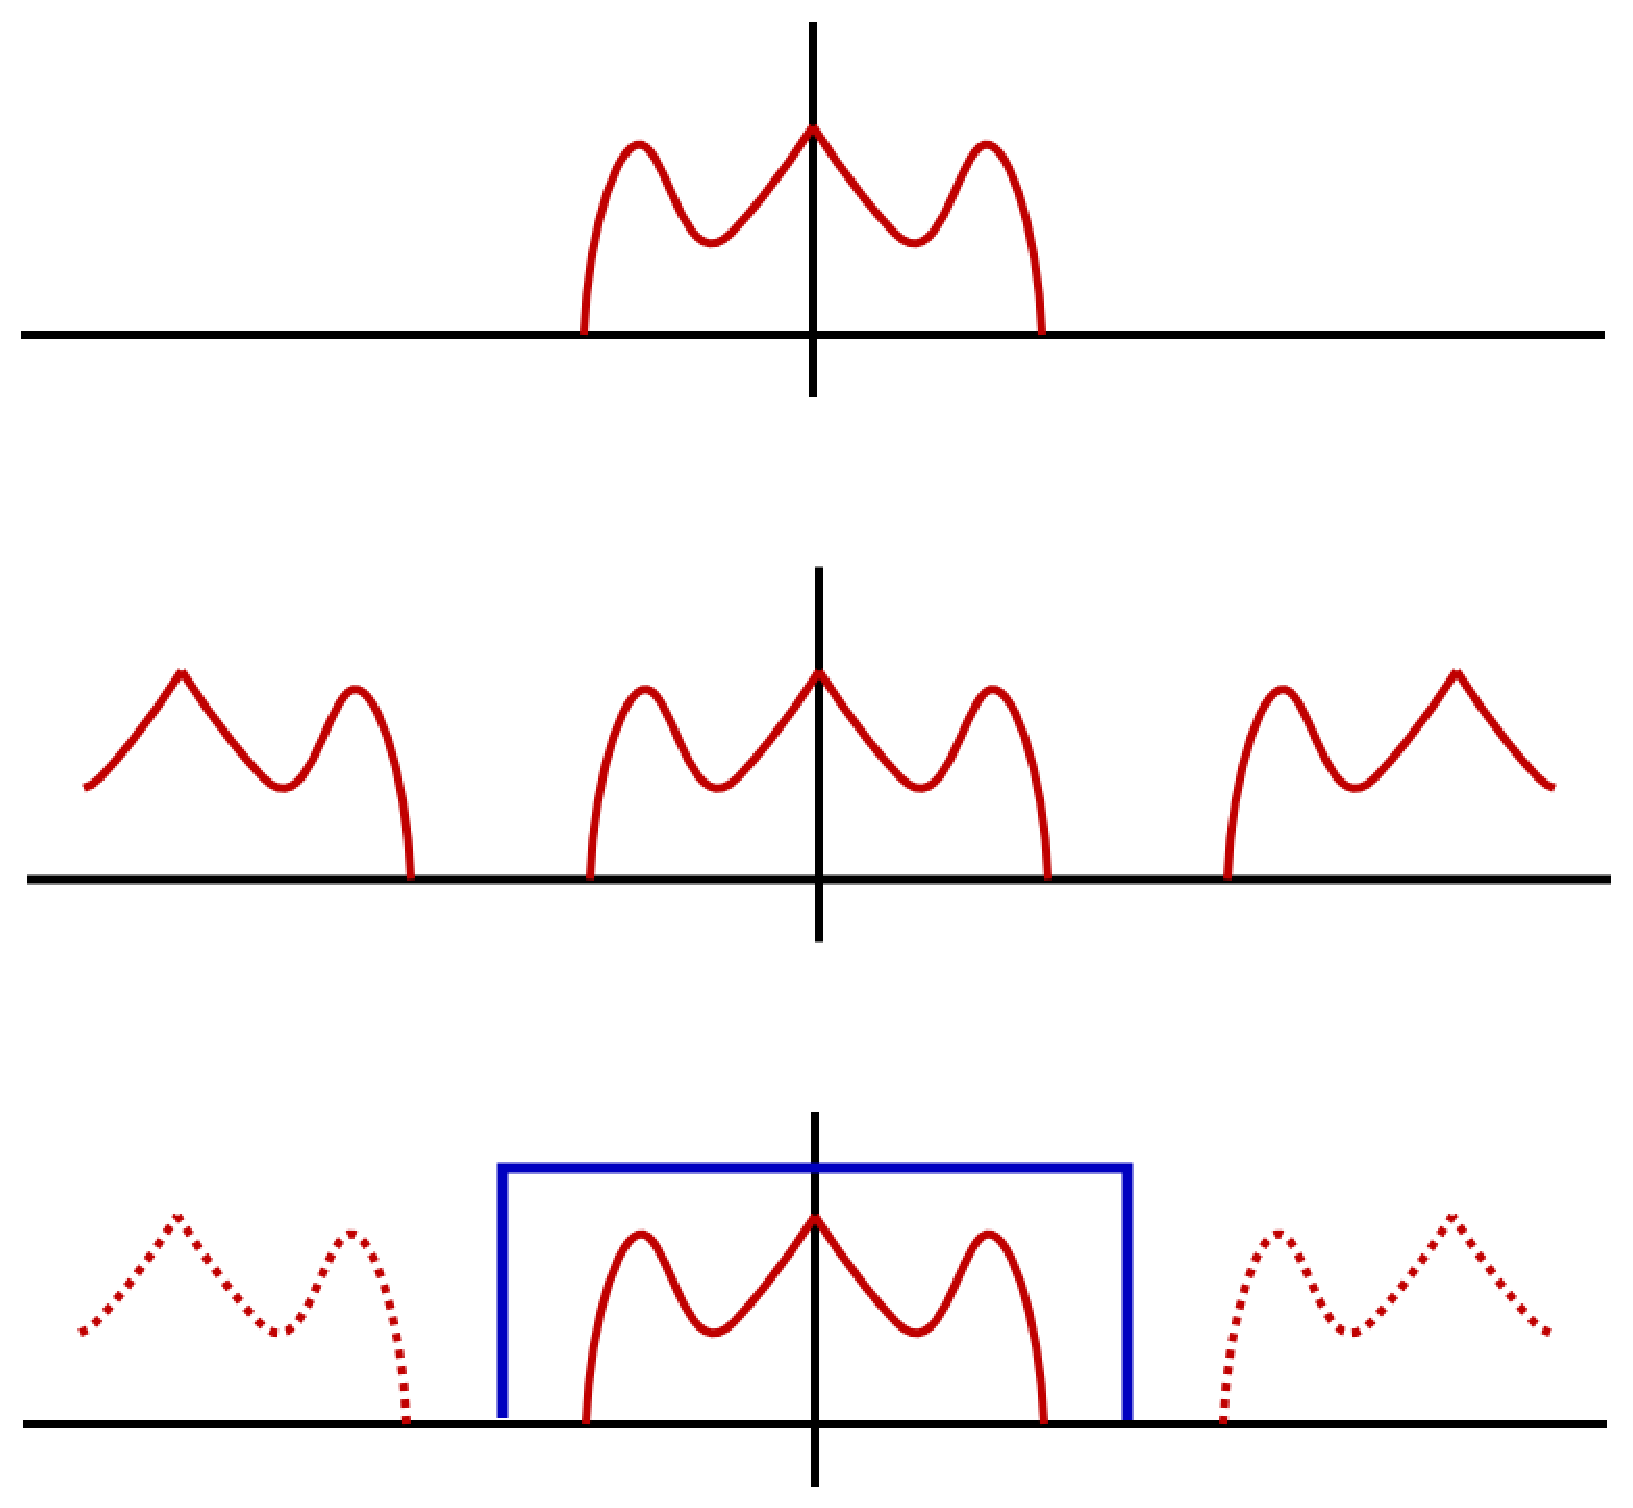
\epsfig{file=Figures/sampling,width=8cm}
\caption{The sampling and reconstruction of a bandwidth-limited signal.
When the sampling rate exceeds twice the bandwidth of the original signal, this signal can be reconstituted from its sampled values.}
\label{figure:Sampling}
\end{center}
\end{figure}
A succession of power spectral densities can be found on Figure~\ref{figure:Sampling}.
The top component shows the power spectral density of the original signal.
The density of the sampled signal appears below.
Finally, the reconstruction operation where a lowpass filter is employed to recovered the original function is illustrated at the bottom of the figure.
In contrast, Figure~\ref{figure:Aliasing} exhibits a case where the sampling frequency is too low.
\begin{figure}[htbp]
\begin{center}
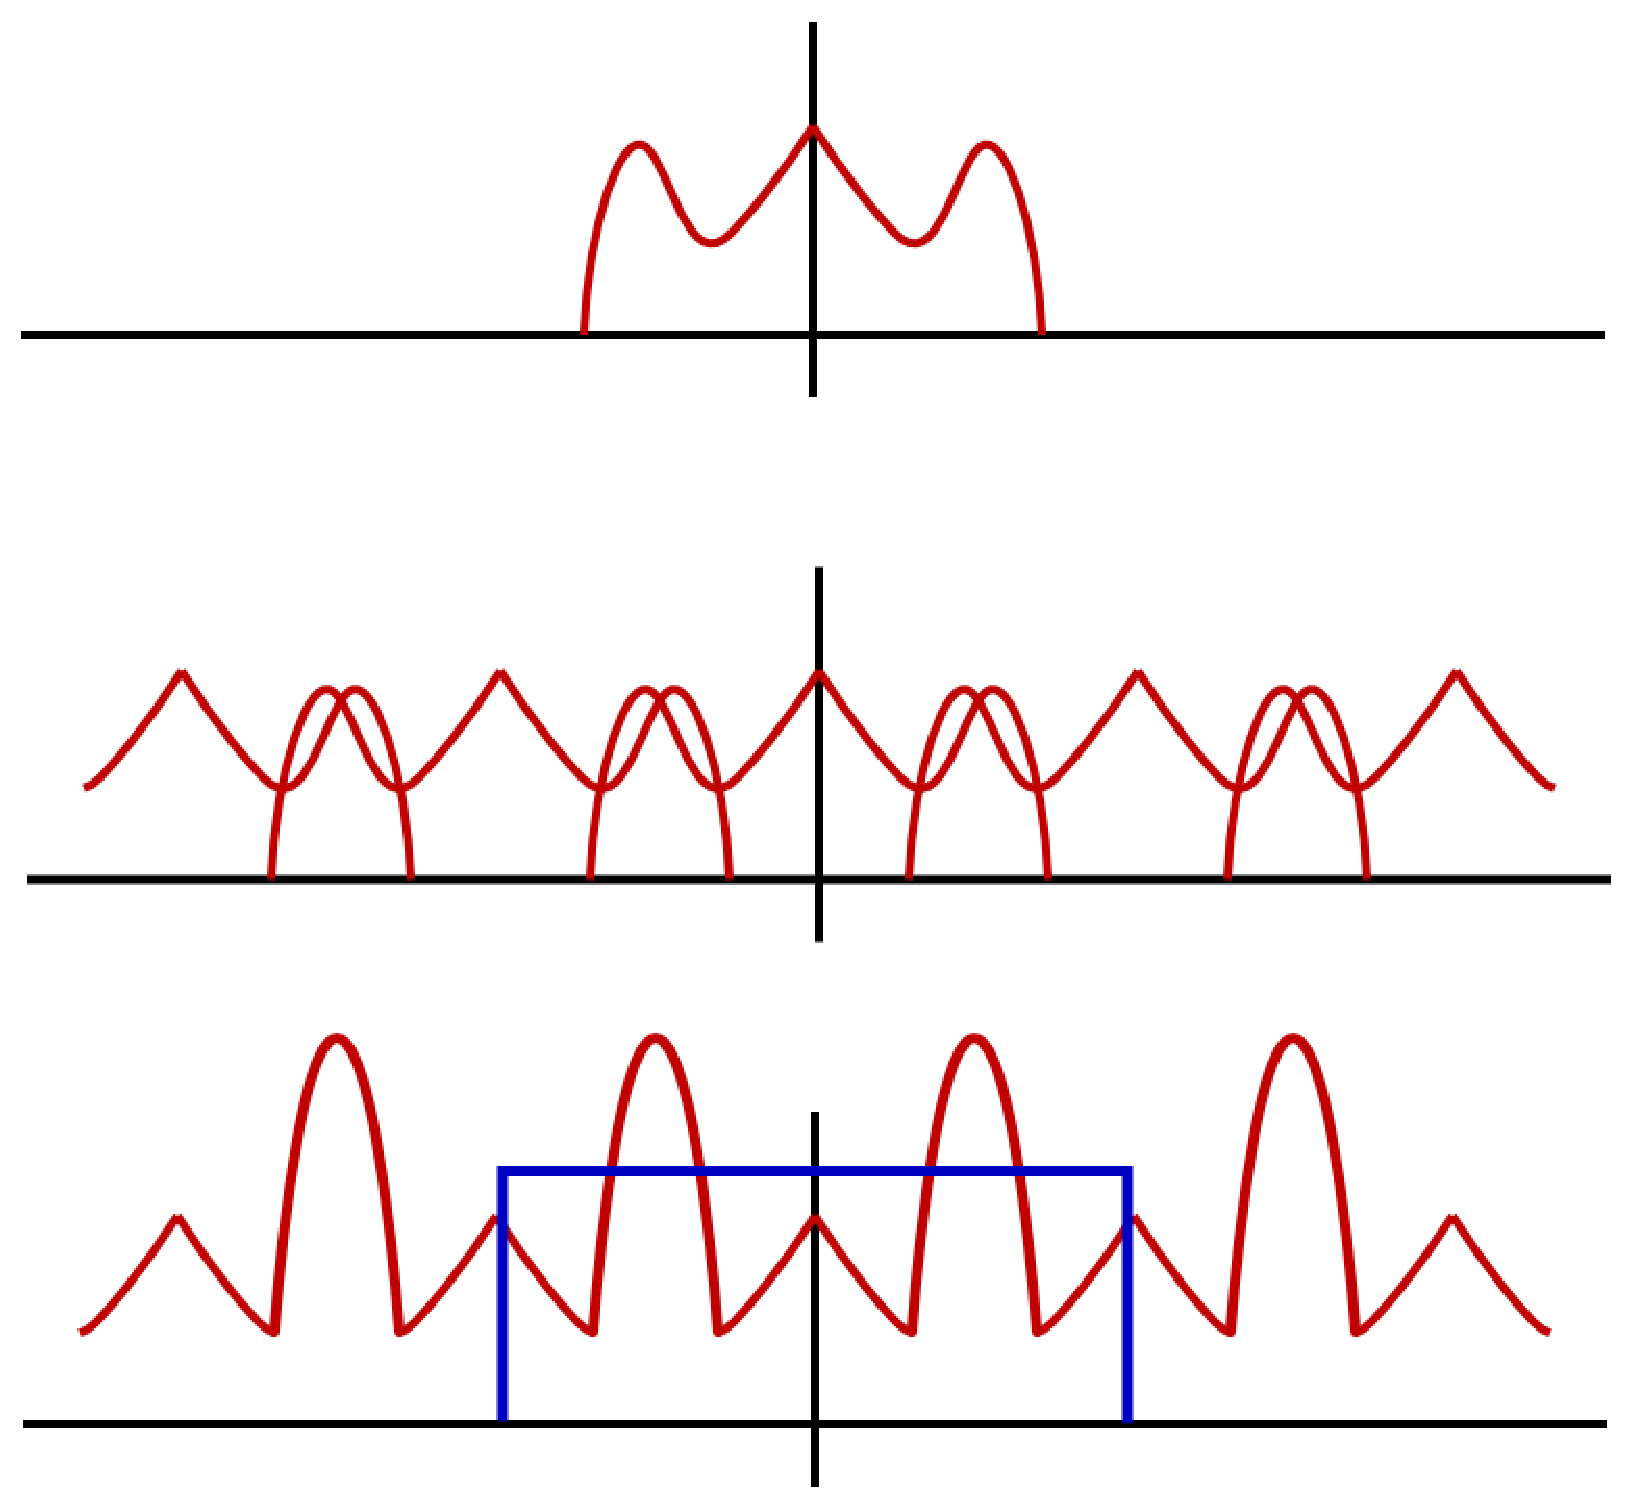
\epsfig{file=Figures/aliasing,width=8cm}
\caption{A low sampling frequency leads to aliasing, thereby preventing reconstruction of the original signal.}
\label{figure:Aliasing}
\end{center}
\end{figure}
Aliasing in the frequency domain prevents the original signal from being retrieved.

The illusion of a moving image in video is achieved by displaying a rapid succession of still pictures over time.
Films are typically shot at a rate of twenty-four frames per second, whereas the minimum frame rate required to create the appearance of a moving image is about fifteen frames per second.
The human eye acts as a lowpass filter and transforms the succession of images into a live video.
High-speed cameras are used to record slow-motion playback movies.
As a consequence, they must run at much higher frame-rates than normal cameras.


\section{Stochastic Signals}
\label{section:StocahsticSignalsFAS}

A \emph{stochastic process} (or \emph{random process}) is an extension of the concept of \emph{random variable} to the situation where the values of a signal are not known beforehand.
Mathematically, a stochastic process can be viewed in two different ways.
First, the process can be thought of as an instantiation of a random experiment where the outcome is selected from a collection of time functions.
Alternatively, a stochastic process can be viewed as a collection of random variables indexed by time.
If the index set corresponds to the real numbers, then the process is a \emph{continuous-time random process}.
Whereas if the index set is discrete, then the random process is a \emph{discrete-time random process}.
The viewpoint where a stochastic process is regarded as a collection of random variables tends to prevail in the study of digital communications.
\begin{figure}[htbp]
\begin{center}
\begin{psfrags}
\psfrag{A}[c]{Amplitude}
\psfrag{t}[c]{Time}
\psfrag{t0}[c]{$t_0$}
\psfrag{t1}[c]{$t_1$}
\epsfig{file=Figures/process,width=7cm}
\end{psfrags}
\caption{Two distinct abstractions of a random process.
It can be viewed as the output of an experiment where a function is selected at random.
Alternatively, a random process may be taken as a set of random variables indexed by time.}
\label{figure:RandomProcess}
\end{center}
\end{figure}

Random processes are frequently employed in the design of communication systems.
For example, they can be used to model the data originating from a source, channel variations, noise and interference.
Their importance will become evident as we progress through these notes.
In general, it is difficult to provide a complete mathematical description for a random process.
For now, we restrict our attention to \emph{stationary} and \emph{ergodic} random processes.

\begin{definition}[Stationarity]
A random process $X(t)$ is wide-sense stationary if its \emph{mean}
\begin{equation*}
m_X(t) = \mathrm{E} [X(t)]
\end{equation*}
is independent of time, and its \emph{autocorrelation function} defined by
\begin{equation*}
R_X(t_1, t_2) = \mathrm{E} [X(t_1) X^*(t_2)]
\end{equation*}
only depends on the difference between $t_1$ and $t_2$.
With a slight abuse of notation, we can denote the mean and autocorrelation of a stationary process respectively by $m_X$ and $R_X(\tau)$, where $\tau = t_1 - t_2$.
\end{definition}

\begin{definition}[Ergodicity]
The \emph{ergodic theorems} assert that, under certain conditions, the time average of a function along all the possible trajectories of a random process exists and is equal to its ensemble average,
\begin{equation*}
\lim_{T \rightarrow \infty} \frac{1}{T} \int_{- \frac{T}{2}}^{\frac{T}{2}} g(X(t)) dt
= \mathrm{E}[g(X(t))] .
\end{equation*}
When a stochastic process fulfills these conditions, it is called \emph{ergodic}.
\end{definition}

\begin{figure}[htbp]
\begin{center}
\begin{psfrags}
\psfrag{A}[c]{Amplitude}
\psfrag{t}[c]{Time}
\psfrag{t0}[c]{$t_0$}
\psfrag{m}[c]{$m_X$}
\psfrag{e}[c]{$\lim_{T \rightarrow \infty} \frac{1}{T} \int_{- \frac{T}{2}}^{\frac{T}{2}} X(t) dt$}
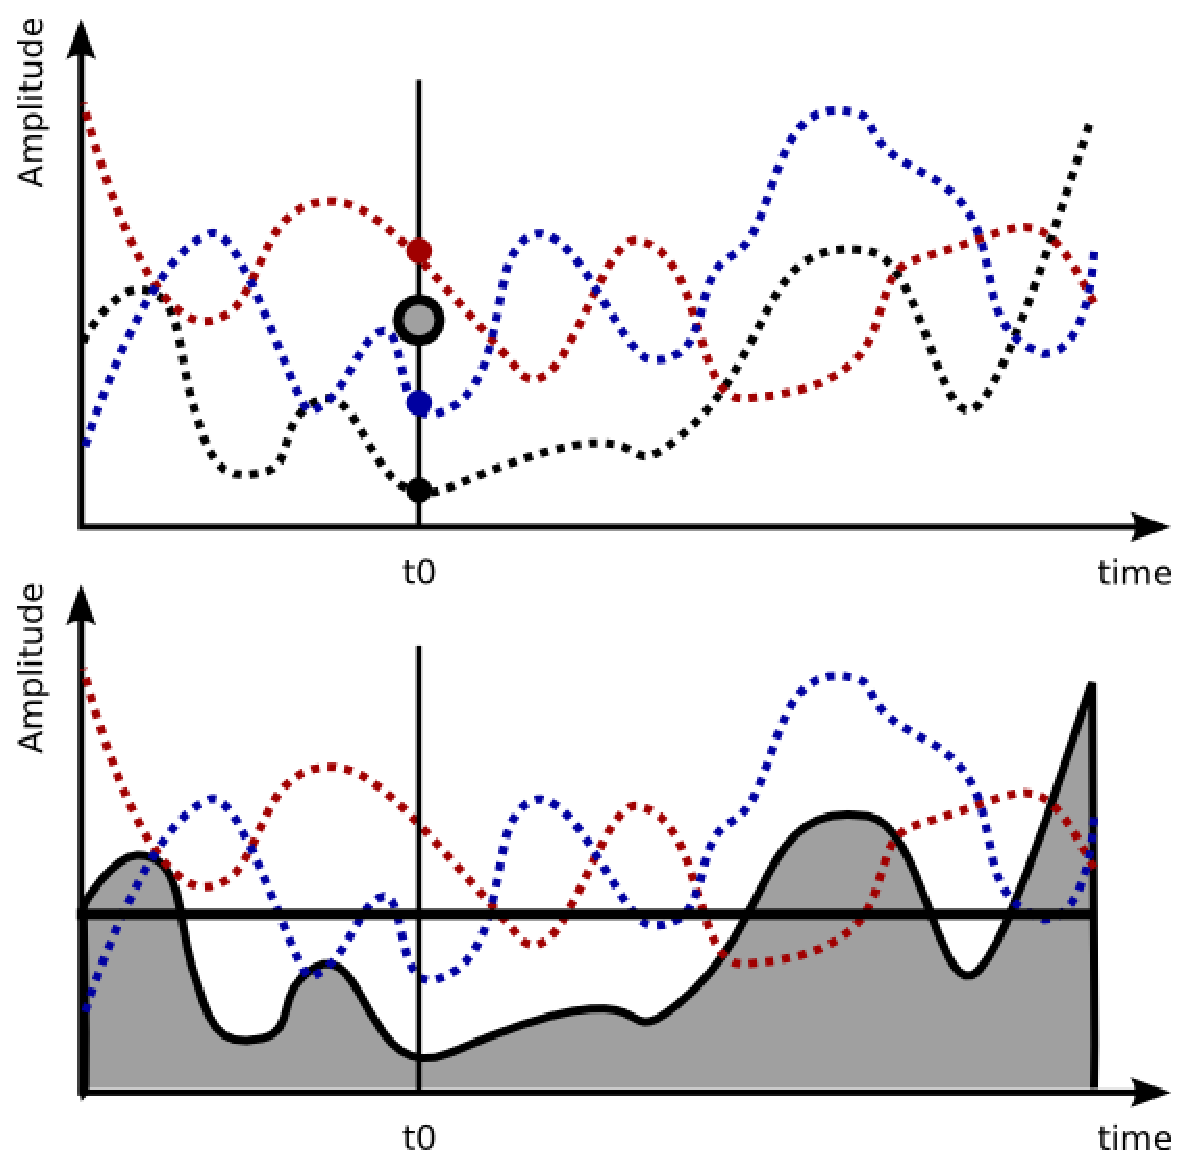
\epsfig{file=Figures/ergodic,width=8cm}
\end{psfrags}
\caption{For ergodic processes, the time average of a function along a trajectory is equal to the ensemble average.}
\label{figure:ErgodicProcess}
\end{center}
\end{figure}

One of the important characteristics of an ergodic process is that it suffices to look at one realization of the process to infer many of its statistical attributes.
Ergodicity is a very strong property, and it is hard to test and validate.
Rather, it is frequently taken as a premise in the design of communication systems.
For instance, most information sources are assumed to be stationary and ergodic.
Such a postulate appears reasonable, especially given the many successful communication systems implemented to date.


\subsection{Power Spectral Density}

The \emph{power spectral density} of a stochastic signal is an extension to the spectral density discussed in Section~\ref{subsection:SpectralDensity}.
The definition of the power spectral density is somewhat more intricate due to the more complex nature of random signals.
In particular, it must account for uncertainty in the process.

Let $X(t)$ be a wide-sense stationary and ergodic random process, with $R_X(0) < \infty$.
The Fourier transform of a specific realization of $x(t)$ may not exist, as it need not fulfill condition \eqref{equation:L2Condition}.
However, a truncated version of $x(t)$ possesses a Fourier transform.
Consider the truncated version of $x(t)$ given by
\begin{equation*}
x_T(t) = x(t) \mathrm{rect} \left( \frac{t}{T} \right) ,
\end{equation*}
and its Fourier transform
\begin{equation*}
\hat{x}_T(f) = \mathcal{F} \left[ x(t) \mathrm{rect} \left( \frac{t}{T} \right) \right] .
\end{equation*}
The power spectral density of $X(t)$ represents the amount of power per hertz of bandwidth present in the signal at various frequencies, and it is defined by
\begin{equation*}
\mathcal{S}_X(f) = \lim_{T \rightarrow \infty} \frac{1}{T} \mathrm{E} \left[ |\hat{x}_T(f)|^2 \right] .
\end{equation*}
Note how the truncated signal is used to overcome the difficulty of dealing with infinite-energy signals.
This is a common and valuable trick.
As we will soon see, the power spectral density plays an instrumental role in the sampling theorem for random signals.
First, we provide a means to compute $\mathcal{S}_X(f)$ from its statistical attributes.

\begin{theorem}[Wiener-Khinchin]
The power spectral density $\mathcal{S}_X (f)$ of a wide-sense stationary random process $X(t)$ is equal to the Fourier transform of its autocorrelation function, $\mathcal{S}_X (f) = \mathcal{F} [R_X (\tau)]$.
\end{theorem}
\begin{proof}
For a wide-sense stationary process, we have
\begin{equation*}
\begin{split}
\mathcal{S}_X(f) &= \lim_{T \rightarrow \infty} \frac{1}{T} \mathrm{E} \left[ |\hat{x}_T(f)|^2 \right]
= \lim_{T \rightarrow \infty} \frac{1}{T} \mathrm{E} \left[ \hat{x}_T(f) \hat{x}_T^*(f) \right] \\
&= \lim_{T \rightarrow \infty} \frac{1}{T} \mathrm{E} \left[
\int_{-\frac{T}{2}}^{\frac{T}{2}} X(t_1) e^{-2 \pi i f t_1} dt_1
\int_{-\frac{T}{2}}^{\frac{T}{2}} X^*(t_2) e^{2 \pi i f t_2} dt_2 \right] \\
&= \lim_{T \rightarrow \infty} \frac{1}{T}
\int_{-\frac{T}{2}}^{\frac{T}{2}} \int_{-\frac{T}{2}}^{\frac{T}{2}}
\mathrm{E} \left[ X(t_1) X^*(t_2) \right]
e^{-2 \pi i f (t_1-t_2)} dt_1 dt_2 \\
&= \int_{\mathbb{R}} R_X (\tau) e^{-2 \pi i f\tau} d\tau
= \mathcal{F} [ R_X (\tau) ] .
\end{split}
\end{equation*}
The fourth equality is obtained by interchanging the expectation and the integrals, while the sixth equality follows from a change of variables and the fact that $X(t)$ is wide-sense stationary.
To guarantee that the former operation is legitimate, $\tau R_X(\tau)$ must remain finite for all $\tau$.
\end{proof}


\subsection{Filtering Stochastic Processes}

We discussed in Section~\ref{subsection:LinearTimeInvariantFilters} how the Fourier transform can simplify the analysis of the effects of linear time-invariant filters on deterministic signals.
In this section, we consider the operation of such filters in the context of random processes.

\begin{theorem}
If a wide-sense stationary process $X(t)$ with mean $m_X$ and autocorrelation function $R_X(\tau)$ is passed through a linear time-invariant filter with impulse response $h(t)$, then the output process $Y(t)$ has mean
\begin{equation*}
m_Y = m_X \int_{\mathbb{R}} h(t) dt
\end{equation*}
and its autocorrelation is equal to
\begin{equation*}
R_Y (\tau) = R_X(\tau) \ast h(\tau) \ast h^*(-\tau) .
\end{equation*}
\end{theorem}
\begin{proof}
The output process at time~$t$ is given by $Y(t) = \int_{\mathbb{R}} X(t - \xi) h(\xi) d\xi$.
We can therefore obtain the expectation of $Y(t)$ as follows,
\begin{equation*}
\begin{split}
m_Y (t) &= \mathrm{E} \left[ \int_{\mathbb{R}} X(t - \xi) h(\xi) d\xi \right]
= \int_{\mathbb{R}} \mathrm{E} \left[ X(t - \xi) \right] h(\xi) d\xi \\
&= m_X \int_{\mathbb{R}} h(\xi) d\xi.
\end{split}
\end{equation*}
We emphasize that $m_Y$ is independent of time.

To derive the autocorrelation function for $Y(t)$, we first compute the cross-correlation between $X(t)$ and $Y(t)$,
\begin{equation} \label{equation:CrossCorrelationLTI}
\begin{split}
\mathrm{E} [X(t_1) Y^*(t_2) ]
&= \mathrm{E} \left[ X(t_1) \int_{\mathbb{R}} X^*(\xi) h^*(t_2 - \xi) d\xi \right] \\
&= \int_{\mathbb{R}} \mathrm{E} \left[ X(t_1) X^*(\xi) \right] h^*(t_2 - \xi) d\xi \\
&= \int_{\mathbb{R}} R_X(t_1 - \xi) h^*(t_2 - \xi) d\xi \\
%&= \int_{\mathbb{R}} R_X(\tau - \xi) h^*(- \xi) d\xi \\
&= R_X(\tau) \ast h^*(-\tau) .
\end{split}
\end{equation}
This shows that the cross-correlation between $X(t)$ and $Y(t)$ depends only on $\tau$; we can therefore express it as $R_{XY}(\tau)$.
We are now ready to compute the autocorrelation function for $Y(t)$.
\begin{equation} \label{equation:AutoCorrelationLTI}
\begin{split}
\mathrm{E} [Y(t_1) Y^*(t_2) ]
&= \mathrm{E} \left[ \int_{\mathbb{R}} X(\xi) h(t_1 - \xi) d\xi Y^*(t_2) \right] \\
&= \int_{\mathbb{R}} \mathrm{E} \left[ X(\xi) Y^*(t_2) \right] h(t_1 - \xi) d\xi \\
&= \int_{\mathbb{R}} R_{XY}(\xi - t_2) h(t_1 - \xi) d\xi \\
%&= \int_{\mathbb{R}} R_{XY}(\xi) h(\tau - \xi) d\xi \\
&= R_{XY}(\tau) \ast h(\tau) .
\end{split}
\end{equation}
Substituting $R_{XY} (\tau)$ by the equivalent expression $R_X(\tau) \ast h^*(-\tau)$ from \eqref{equation:CrossCorrelationLTI}, we get the desired result.
We observe that the autocorrelation of the process $Y(t)$ only depends on the difference between $t_1$ and $t_2$, and hence $Y(t)$ is also wide-sense stationary.
\end{proof}

Obtaining an expression for the autocorrelation function corresponding to the output of a linear time-invariant filter allows us to characterize the power spectral density of the output process.
In terms of the frequency representation, we get $m_Y = m_X \hat{h}(0)$ and
\begin{equation*}
\begin{split}
\mathcal{S}_Y (f) &= \mathcal{F} [ R_Y (\tau) ] \\
&= \mathcal{F} \left[ R_X (\tau) \ast h(\tau) \ast h^*(-\tau) \right] \\
&= \mathcal{S}_X(f) | \hat{h}(f) |^2 .
\end{split}
\end{equation*}
A linear time-invariant filter can be employed to shape the spectrum of a stochastic process, and to constrain its bandwidth.
This is an important result, as linear filters can be used to reduce the bandwidth of a random signal before sampling or to reconstruct a random signal from its samples.


\section{Sampling Bandlimited Processes}

We know from Theorem~\ref{theorem:SamplingTheorem} that a bandwidth-limited signal can be perfectly reconstructed from its samples provided that the sampling rate exceeds twice the bandwidth of the original signal.
At this point, one may wonder whether it is possible to extend the sampling theorem to bandwidth-limited stochastic processes.
This question is answered in the affirmative below.

\begin{theorem} \label{theorem:SamplingRandomSignals}
Suppose that $X(t)$ is a wide-sense stationary bandwidth-limited process with bandwidth $W$ and power spectral density $\mathcal{S}_X (f)$.
Let $\tilde{X}(t)$ be an approximation for $X(t)$ built from the sampled values $\{ X(nT) : n \in \mathbb{Z} \}$,
\begin{equation*}
\tilde{X}(t) = \sum_{n=-\infty}^{\infty} X(nT) \mathrm{sinc} (2 W (t - nT)) ,
\end{equation*}
where $T = \frac{1}{2W}$ denotes the sampling interval.
Then the mean-squared error between the original random process and the reconstructed version vanishes,
\begin{equation} \label{equation:SamplingMSE}
\left\| X(t) - \tilde{X}(t) \right\|^2
= \mathrm{E} \left[ \left| X(t) - \sum_{n=-\infty}^{\infty}
X(nT) \mathrm{sinc} (2 W (t - nT)) \right|^2 \right] = 0 .
\end{equation}
The expectation in \eqref{equation:SamplingMSE} is over all possible realizations of $X(t)$.
\end{theorem}
\begin{proof}
To establish this result, we expand the mean-squared error of \eqref{equation:SamplingMSE},
\begin{equation*}
\begin{split}
&\left\| X(t) - \tilde{X}(t) \right\|^2
= \mathrm{E} \left[ \left| X(t) - \sum_{n=-\infty}^{\infty} X(nT)
\mathrm{sinc}(2 W (t - nT)) \right|^2 \right] \\
&= R_X(0) - \sum_{n=-\infty}^{\infty} [ R_X(t-nT) + R_X^*(t-nT) ]
\mathrm{sinc}(2 W (t - nT)) \\
&+ \sum_{n=-\infty}^{\infty} \sum_{m=-\infty}^{\infty} R_X((m-n)T)
\mathrm{sinc}(2 W (t - mT)) \mathrm{sinc}(2 W (t - nT)) .
\end{split}
\end{equation*}
The double summation above can be rewritten as
\begin{equation*}
\begin{split}
&\sum_{n=-\infty}^{\infty} \sum_{k=-\infty}^{\infty} R_X(kT)
\mathrm{sinc}(2 W (t - kT - nT)) \mathrm{sinc}(2 W (t - nT)) \\
&\sum_{n=-\infty}^{\infty} \left( \sum_{k=-\infty}^{\infty} R_X(kT)
\mathrm{sinc}(2 W (t - kT - nT)) \right) \mathrm{sinc}(2 W (t - nT)) \\
&= \sum_{n=-\infty}^{\infty} R_X(t - nT) \mathrm{sinc}(2 W (t - nT)) ,
\end{split}
\end{equation*}
where the last equality follows from the sampling theorem for deterministic signals (Theorem~\ref{theorem:SamplingTheorem}).
Putting these results together, we get
\begin{equation*}
\left\| X(t) - \tilde{X}(t) \right\|^2
= R_X(0) - \sum_{n=-\infty}^{\infty} R_X^*(t-nT) \mathrm{sinc}(2 W (t - nT)) .
\end{equation*}
Applying Theorem~\ref{theorem:SamplingTheorem} one more time and noticing that $R_X(0) = R_X^*(0)$, we obtain $\| X(t) - \tilde{X}(t) \|^2 = 0$, as desired.
\end{proof}

Theorem~\ref{theorem:SamplingRandomSignals} is important because it confirms that the design insights gained from analyzing deterministic signals hold for random signals as well.


\section{Bandpass Signals and Processes}

One possible application of sampling is to take a continuous-time signal and to transform it into a discrete-time signal.
For instance, this operation gives the information coming out of a source a format more suitable for digital communications.
This prime application of sampling served as the original motivation for our study of the subject.
A second possible application of sampling is the processing of received waveforms at the output of communication channels.
In digital communications, the data often assumes the form of an analog carrier signal modulated by a digital bit stream.
Mathematically, this situation is captured by the equation
\begin{equation*}
y(t) = x(t) \cos (2 \pi f_{\mathrm{c}} t) .
\end{equation*}
The signal $y(t)$ is a special form of a \emph{bandpass signal}.
Its Fourier transform $\hat{y}(f)$ is non-zero only for frequencies contained in a small neighborhood of carrier frequency $f_{\mathrm{c}}$.
That is, $\hat{y}(f) = 0$ for all frequencies such that $|f - f_{\mathrm{c}}| \geq W$.
To apply the sampling tools derived above to the information bearing signal $x(t)$, we need to shift the corresponding spectrum to the origin.

The Fourier transform of $y(t)$ is given by
\begin{equation*}
\hat{y}(f) = \frac{1}{2} \hat{x}(f+f_{\mathrm{c}}) + \frac{1}{2} \hat{x}(f - f_{\mathrm{c}}) .
\end{equation*}
Our strategy is to first eliminate $\frac{1}{2} \hat{x}(f + f_{\mathrm{c}})$ from $\hat{y}(f)$, and then to scale and shift $\frac{1}{2} \hat{x}(f + f_{\mathrm{c}})$ back to the origin.
Define the \emph{step function} by
\begin{equation*}
\mathrm{step} (t) = \frac{1}{2} + \frac{1}{2} \mathrm{sign}(t). 
\end{equation*}
Taking the (cavalier) Fourier transform of $\mathrm{step}(t)$, we get
\begin{equation*}
\begin{split}
{\mathcal{F}} [\mathrm{step} (t)]
&= {\mathcal{F}} \left[ \frac{1}{2} + \frac{1}{2} \mathrm{sign}(t) \right] \\
&= \frac{1}{2} \delta (f)
- \frac{1}{2} \int_{-\infty}^0 e^{-2 \pi i ft} dt
+ \frac{1}{2} \int_0^{\infty} e^{-2 \pi i ft} dt \\
&= \frac{1}{2} \delta(f)  + \frac{1}{2 \pi i f}.
\end{split}
\end{equation*}
Using the duality property of the Fourier transform, we get
\begin{equation*}
\mathcal{F}^{-1} [\mathrm{step}(f)] = \frac{1}{2} \delta(t) + \frac{i}{2 \pi t} .
\end{equation*}
And, by construction, we obtain $\hat{x}(f - f_{\mathrm{c}}) = 2 \mathrm{step}(f) \hat{y}(f)$.
We can therefore recover the original lowpass signal $x(t)$ using the frequency-shift property of the Fourier transform,
\begin{equation*}
x(t)
= \left[ y(t) \ast \left( \delta (t) + \frac{i}{\pi t} \right) \right]
e^{- 2 \pi i f_{\mathrm{c}} t}
= \left[ y(t) + i \left( y(t) \ast \frac{1}{\pi t} \right) \right] e^{- 2 \pi i f_{\mathrm{c}} t} .
\end{equation*}
The second component of this signal,
\begin{equation*}
y(t) \ast \frac{1}{\pi t} ,
\end{equation*}
is called the \emph{Hilbert transform} of $y(t)$.
Once $x(t)$ is brought back to baseband, the standard sampling theorem applies and a discrete-time version of the signal can be produced.

% Bandpass processes

\chapter{Quantization}

As mentioned in the introduction, two operations are necessary to transform an analog waveform into a digital signal.
The first action, discussed in Chapter~\ref{chapter:FourierAnalysisSampling}, is called sampling.
It consists of converting a continuous-time input into a discrete-time signal.
The second operation is the process of approximating continuous-space samples by a discrete set of possible symbols.
This process termed \emph{quantization} is equally essential in order to transmit an analog signal over digital media.
Quantization invariably induces a loss in signal quality.
The \emph{distortion} between the original and quantized signals is usually unwanted, and cannot be reversed.
Yet, for a specific application, the level of signal degradation can be controlled.


\section{Scalar Quantizers}

Generic quantizers operate on large classes of signals and are very robust.
In scalar quantization, each source value is processed individually, with the quantizer output taking one of finitely many possibilities.
The number of quantization levels tends to be a base-two exponent because the output of the quantizer is often represented using binary symbols.
Mathematically, a quantizer can be expressed as a function.
Suppose that the input to the quantizer is a real number, and its output is a value that belongs to the set $\mathcal{Q}$.
Then we can describe the quantizer as a function $Q : \mathbb{R} \mapsto \mathcal{Q}$ with output
\begin{equation*}
x_{\mathrm{q}} = Q(x) .
\end{equation*}
This is perhaps best seen through an example.


\begin{example}
Let $Q : \mathbb{R} \mapsto \mathcal{Q}$ be a quantizer with four possible outputs labeled $q_1$ through $q_4$.
The output $x_{\mathrm{q}}$ of the quantizer belongs to set $\mathcal{Q}$, and it must therefore be equal to one of the four possible points listed above.
Figure~\ref{figure:Quantizer} shows the functional representation of a four-level quantization scheme.
\begin{figure}[htbp]
\begin{center}
\begin{psfrags}
\psfrag{q1}[l]{$q_1$}
\psfrag{q2}[l]{$q_2$}
\psfrag{q3}[l]{$q_3$}
\psfrag{q4}[l]{$q_4$}
\psfrag{o}[c]{Output}
\psfrag{i}[c]{Input}
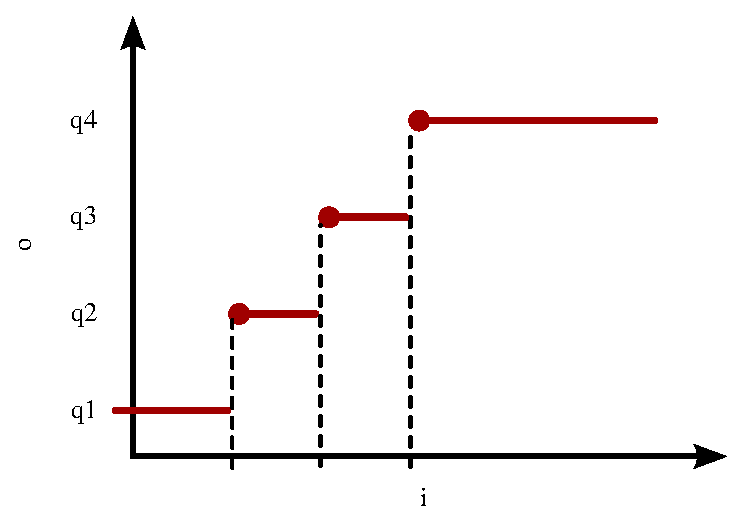
\epsfig{file=Figures/quantizer,width=6cm}
\end{psfrags}
\caption{A functional representation of a quantizer.}
\label{figure:Quantizer}
\end{center}
\end{figure}

The output of the quantizer in this example is determined according to a nearest neighbor rule.
Note that this function is not injective (one-to-one) and, as such, has no inverse.
\end{example}


\section{Distortion Measures}

To compare different quantizers, a performance metric must be established.
A common distortion criterion with nice properties is the square of the error
\begin{equation} \label{equation:QuantizationErrorSquared}
d(x, x_{\mathrm{q}}) = (x - Q(x))^2 = e_{\mathrm{q}}^2 ,
\end{equation}
where $e_{\mathrm{q}} = x - x_{\mathrm{q}}$ is the \emph{quantization error}.
The criterion in \eqref{equation:QuantizationErrorSquared} specifies how close the output $x_{\mathrm{q}}$ is to $x$ for a specific realization of $x$.
Since the quantizer is designed to operate on an information signal, a more relevant assessment of performance weighs in the accuracy of the quantizer over all possible realizations of the input.
An appropriate distortion measure for the quantization of a random signal is provided by the \emph{mean squared error (MSE)},
\begin{equation} \label{equation:QuantizationMSE}
\mathrm{E} [ d(X, X_{\mathrm{q}}) ]
= \mathrm{E} \left[ (X - Q(X))^2 \right] = \| E_{\mathrm{q}} \|^2 .
\end{equation}
Note that this performance metric depends on the distribution of the input signal, and hence is tied to a specific application.
A quantizer can be said to work well in a particular context.
However, describing the performance of a quantization scheme without specifying the properties of its input signal is meaningless.

\begin{example} \label{example:UniformQuantizer}
Suppose that the values of a discrete-time information signal are uniformly distributed over $[0,16]$.
Furthermore, assume that the quantizer implements a nearest neighbor rule with quantization levels equal to $q_i = 2i - 1$ for $i = 1, 2, \ldots, 8$.
We wish to find the mean squared error of this quantization scheme.

Being uniformly distributed, the probability density function of the input signal is
\begin{equation*}
f_X (\xi) = \frac{1}{16}
\end{equation*}
for $\xi \in [0, 16]$, and zero otherwise.
The decision regions corresponding to the various quantization points are then given by $[0, 2], (2, 4], \ldots, (14, 16]$.
We can therefore compute the mean squared error as follows,
\begin{equation*}
\begin{split}
\mathrm{E} [ d(X, X_{\mathrm{q}}) ]
&= \mathrm{E} \left[ (X - Q(X))^2 \right]
= \int_0^{16} \frac{(\xi - Q(\xi))^2}{16} d\xi \\
&= \sum_{i=1}^8 \int_{2i-2}^{2i} \frac{(\xi - (2i - 1))^2}{16} d\xi \\
&= \frac{1}{2} \int_{0}^{2} (\xi - 1)^2 d\xi = \frac{1}{3} .
\end{split}
\end{equation*}
That is, the mean squared error associated with this input distribution and quantization scheme is $\| e_{\mathrm{q}} \|^2 = \frac{1}{3}$.
\end{example}

One of the criticisms about the MSE of \eqref{equation:QuantizationMSE} is that it has a tendency to assign a larger distortion value to signal input with sizable second moments.
Indeed, an information process likely to feature large amplitudes is bound to yield outputs with a large mean squared error.
On the other hand, under this absolute metric, most quantizers may appear to work well for minute signals as their mean square errors are destined to remain small.
An alternative and closely related criterion that takes into consideration the power of the original signal is the \emph{signal-to-quantization-noise ratio (SQNR)},
\begin{equation} \label{equation:SQNR}
\text{SQNR} = \frac{\| X \|^2}{\| e_{\mathrm{q}} \|^2}
= \frac{\mathrm{E} \left[ X^2 \right]}{\mathrm{E} \left[ (X - Q(X))^2 \right]} .
\end{equation}
Because of the implicit normalization associated with \eqref{equation:SQNR}, this latter performance measure is more suitable to compare quantizer performance for different input processes.

\begin{example}
This time, assume that the values of a discrete-time information signal are uniformly distributed over $[0,2]$.
To avoid confusion, we denote the input signal in the present problem using $Y$.
We wish to obtain the mean squared error associated with the quantizer of Example~\ref{example:UniformQuantizer}, applied to the signal at hand.
Also, we wish to compare the SQNR of the quantization scheme of Example~\ref{example:UniformQuantizer} with the SQNR of the scenario described in this example.

To derive the mean squared error, we follow the same steps as before
\begin{equation*}
\begin{split}
\mathrm{E} [ d(Y, Y_{\mathrm{q}}) ]
&= \int_0^{2} \frac{(\zeta - Q(\zeta))^2}{2} d\zeta \\
&= \frac{1}{2} \int_{0}^{2} (\zeta - 1)^2 d\zeta = \frac{1}{3} .
\end{split}
\end{equation*}
We notice that the MSE is the same as the one derived in Example~\ref{example:UniformQuantizer}.
Nevertheless, the quantization scheme seems more suited to the signal described in the previous example.
The SQNR of the current scheme is given by
\begin{equation*}
\text{SQNR} = \frac{\| Y \|^2}{\mathrm{E} [ d(Y, Y_{\mathrm{q}}) ]}
= 3 \| Y \|^2 = 4.
\end{equation*}
This can be compared with the SQNR of the problem featured in Example~\ref{example:UniformQuantizer}, which is given by
\begin{equation} \label{equation:UniformQuantizerSQNR}
\text{SQNR} = \frac{\| X \|^2}{\mathrm{E} [ d(X, X_{\mathrm{q}}) ]}
= 3 \| X \|^2 = 256.
\end{equation}
Obviously, the SQNR is much better in the case of Example~\ref{example:UniformQuantizer}.
Can you think of an eight-level quantization scheme that would perform better for the current problem, perhaps rivaling the SQNR of \eqref{equation:UniformQuantizerSQNR}?
\end{example}

Both the mean squared error and the signal-to-quantization-noise ratio are valid and meaningful ways to present performance results for quantization schemes.
Still, they must be put in proper context, especially when comparing scenarios where the distributions of the input signals differ.
For a fixed input process, a quantization scheme that minimizes the MSE will invariably maximize the SQNR.


\section{Uniform Quantizers}
\label{section:UniformQuantizers}

Finding an optimal quantizer is not an easy task.
An eight-level quantizer has eight degrees of freedom, and the overall performance of the quantizer is jointly determined by the positions of the quantization points.
A means to reduce the difficulty of identifying an optimal quantization scheme is to constraint the possible candidates.
This can be achieved, for instance, by imposing a rule on the respective position of the quantization points.
Restricting the search space to uniform quantizers is one possible way to ensure that an optimal quantizer can be found.

A \emph{uniform quantizer} is a function where the locations of successive outputs are situated at a fixed interval, $q_i - q_{i-1} = \Delta$ for all the possible values.
That is, the distance between two quantization points is the same for all neighbors.
This scheme is one of the simplest quantizer designs.
The quantization function considered in Figure~\ref{figure:Quantizer} is in fact a uniform quantizer.
If the objective function of the optimization process is the mean squared error, then optimal locations for the quantization points can be found in a straightforward manner.
First, note that we can write the position of the quantization points as
\begin{equation*}
q_i = q_1 + (i-1) \Delta
\end{equation*}
for $i = 1, 2, \ldots, \ell$ where $\ell$ is the number quantization levels.
As usual, the MSE is given by
\begin{equation*}
\mathrm{E} [ d(X, X_{\mathrm{q}}) ]
= \int_{-\infty}^{\infty} (\xi - Q(\xi))^2 f_X(\xi) d\xi .
\end{equation*}
We emphasize  that the performance of the quantizer is optimized by minimizing the value of the integrand at each point.
We deduce that the decision regions corresponding to $q_1, q_2, \ldots, q_{\ell}$ must be equal to
\begin{equation*}
\left( - \infty, q_1 + \frac{\Delta}{2} \right],
\left( q_2 - \frac{\Delta}{2}, q_2 + \frac{\Delta}{2} \right],
\ldots,
\left( q_{\ell} - \frac{\Delta}{2}, \infty \right) ,
\end{equation*}
respectively.
The objective function then becomes
\begin{equation} \label{equation:UniformQuantizerMSE}
\begin{split}
\text{MSE} &= \int_{-\infty}^{q_1 + \frac{\Delta}{2}} (\xi - q_1)^2 f_X(\xi) d\xi
+ \sum_{i=2}^{{\ell}-1}
\int_{q_i - \frac{\Delta}{2}}^{q_i + \frac{\Delta}{2}}
(\xi - q_i)^2 f_X(\xi) d\xi \\
&+ \int_{q_{\ell} - \frac{\Delta}{2}}^{\infty} (\xi - q_{\ell})^2 f_X(\xi) d\xi .
\end{split}
\end{equation}
The resulting optimization process now has two degrees of freedom, namely $q_1$ and $\Delta$.
For a suitable probability density function $f_X(\cdot)$, an optimal solution can be obtained explicitly using standard optimization methods.

\begin{example} \label{example:OptimalUniformQuantizer}
We revisit Example~\ref{example:UniformQuantizer} in the context of uniform quantizers.
Again, suppose that the values of the discrete-time input process are uniformly distributed over $[0, 16]$.
We wish to find the optimal eight-level uniform quantizer associated with this input distribution.

For simplicity, we assume that the quantization points $\{ q_1, q_2, \ldots, q_8 \}$ are contained in the interval $[0, 16]$.
This implies that $q_1 > 0$ and $q_8 < 16$.
The mean squared error as a function of $q_1$ and $\Delta$ is given by \eqref{equation:UniformQuantizerMSE}, which becomes
\begin{equation*}
\begin{split}
\text{MSE}~(q_1, \Delta)
%&= \int_{0}^{q_1 + \frac{\Delta}{2}} \frac{(\xi - q_1)^2}{16} d\xi
%+ \sum_{i=2}^{7}
%\int_{q_i - \frac{\Delta}{2}}^{q_i + \frac{\Delta}{2}}
%\frac{(\xi - q_i)^2}{16} d\xi
%+ \int_{q_8 - \frac{\Delta}{2}}^{16} \frac{(\xi - q_8)^2}{16} d\xi \\
&= \int_{-q_1}^{\frac{\Delta}{2}} \frac{\xi^2}{16} d\xi
+ 6 \int_{- \frac{\Delta}{2}}^{\frac{\Delta}{2}} \frac{\xi^2}{16} d\xi
+ \int_{- \frac{\Delta}{2}}^{16 - q_8} \frac{\xi^2}{16} d\xi \\
\end{split}
\end{equation*}
Recall that, by construction, we can write $q_8 = q_1 + 7 \Delta$.
Taking first derivatives with respect to $q_1$ and $\Delta$, we obtain
\begin{align*}
\frac{\partial}{\partial q_1} \text{MSE}~(q_1, \Delta)
&= \frac{q_1^2}{16} - \frac{(16 - q_1 - 7 \Delta)^2}{16} \\
\frac{\partial}{\partial \Delta} \text{MSE}~(q_1, \Delta)
&= \frac{7 \Delta^2}{64} - \frac{7 (16 - q_1 - 7\Delta)^2}{16} .
\end{align*}
Setting these derivatives equal to zero, we get $q_1 = 1$ and $\Delta = 2$.
A second derivative test ensures that this corresponds to a local minimum.
Since this point is the only inflection point of the function $\text{MSE}~(q_1, \Delta)$ within our search space, we gather that the quantization scheme of Example~\ref{example:UniformQuantizer} coincide with the optimal uniform quantizer.
\end{example}

Although the search space for uniform quantizers is much smaller than the set of all possible quantizers, finding an optimal uniform quantizer remains a strenuous task in most situations.
The resulting minimization problem need not have a closed-form solution, in contrast to Example~\ref{example:OptimalUniformQuantizer}.
This task is often accomplished by discretizing the search space and applying numerical techniques to identify the best candidate.


\section{Non-Uniform Quantizers}
\label{section:NonUniformQuantizers}

For a \emph{non-uniform quantizer}, the restriction that neighboring quantization points should be equidistant from one another is removed.
As such, these points can be located anywhere on the real line, and the decision region corresponding to each quantization point need not have a simple structure.
The collection of non-uniform quantizers is much larger then the set of uniform quantizers described in Section~\ref{section:UniformQuantizers}.
This greater flexibility in choosing a quantizer often results in better overall performance.
However, it also comes with added complexity in designing the quantization scheme.
In this section, we explore some properties of an optimal quantizer for the mean squared error criterion and we present an algorithm that can be employed to obtain a non-uniform quantizer.

First, suppose that the quantization points $\{ q_i \}$ are fixed.
An optimal quantizer for these points is a function $Q^* : \mathbb{R} \mapsto \mathcal{Q}$ that minimizes the corresponding MSE,
\begin{equation*}
\begin{split}
\min_Q \mathrm{E} [ d(X, X_{\mathrm{q}}) ]
&= \min_Q \int_{-\infty}^{\infty} (\xi - Q(\xi))^2 f_X(\xi) d\xi \\
&= \int_{-\infty}^{\infty} \min_{Q(\xi)} (\xi - Q(\xi))^2 f_X(\xi) d\xi .
\end{split}
\end{equation*}
The last equality follows from the fact that a quantization point can be selected independently for every possible input value.
It should then be clear that the value of the function $Q^*(\cdot)$ evaluated at $x$ is the point $q_i$ that is closest to $x$,
\begin{equation*}
Q^*(x) = \arg \min_{\{ q_i \}} (x - q_i)^2 .
\end{equation*}
In particular, an optimal $\ell$-level scalar quantizer always has $\ell$ decision regions, each being an interval containing its quantization point.

Also, we can assume that the decision intervals are given.
Let the boundaries of these intervals be denoted by $b_1, b_2, \ldots, b_{\ell-1}$.
Then, the corresponding MSE is given by
\begin{equation} \label{equation:BoundaryQuantizationMSE}
\int_{-\infty}^{b_1} (\xi - q_1)^2 f_X(\xi) d\xi
+ \sum_{i=2}^{{\ell}-1}
\int_{b_{i-1}}^{b_i} (\xi - q_i)^2 f_X(\xi) d\xi
+ \int_{b_{\ell-1}}^{\infty} (\xi - q_{\ell})^2 f_X(\xi) d\xi .
\end{equation}
The value of the MSE can be minimized by selecting the quantization points $\{ q_i \}$ appropriately.
Note that each quantization point can be optimized individually, as the integrals in \eqref{equation:BoundaryQuantizationMSE} have a nice additive structure.
Solving one instance of the decoupled problem, we get
\begin{equation*}
q_i^* = \min_{q_i} \int_{b_{i-1}}^{b_i} (\xi - q_i)^2 f_X(\xi) d\xi .
\end{equation*}
To obtain the solution, we differentiate the objective function with respect to $q_i$ and set the derivative equal to zero;
\begin{equation*}
\frac{d}{d q_i} \int_{b_{i-1}}^{b_i} (\xi - q_i)^2 f_X(\xi) d\xi
= - \int_{b_{i-1}}^{b_i} 2 (\xi - q_i) f_X(\xi) d\xi = 0 .
\end{equation*}
This implies that
\begin{equation*}
q_i^* = \mathrm{E} [ X | b_{i-1} < X \leq b_i ] .
\end{equation*}
Once the decision intervals are picked, the optimal quantization point $q_i^*$ is equal to the expectation of $X$ conditioned on $X$ falling inside interval~$i$.

Putting these two observations together, we can summarized the properties of an optimal $\ell$-level quantizer as follows.
Suppose that $Q^* : \mathbb{R} \mapsto \mathcal{Q}$ is an optimal quantizer with respect to the mean square error criterion (or the signal-to-quantization-noise ratio).
Then, the decision regions corresponding to the quantization points $\{ q_i \}$ form a partition of the real line where each decision set is an interval.
Given the positions of the various quantization points $\{ q_i \}$, the boundaries of the decision intervals are given by
\begin{equation*}
b_i = \frac{q_i + q_{i+1}}{2}
\end{equation*}
where $i = 1, 2, \ldots, \ell-1$.
Furthermore, the quantization point corresponding to decision interval $(b_{i-1}, b_i]$ is equal to the expectation of $X$ conditioned on $b_{i-1} < X \leq b_i$.
These properties are collectively known as the \emph{Lloyd-Max} conditions.


\subsection{Lloyd-Max Algorithm}

The Lloyd-Max conditions enumerated above form a set of rules that are necessarily fulfilled by optimal quantizers.
Yet, they do not provide an explicit means to compute the exact positions of the quantization points in an optimal quantizer.
Furthermore, it may not be possible to find these points analytically.

A method that is frequently used to find a non-uniform scalar quantizer is the \emph{Lloyd-Max algorithm}.
This algorithm starts with an initial assignment for the quantization points which, in this case, we label $q_1^{(0)}, q_2^{(0)}, \ldots, q_{\ell}^{(0)}$.
The ensuring procedure is to alternate iteratively between the following two steps.
\begin{enumerate}
\item Compute the boundaries of the decision intervals according to
\begin{equation*}
b_i^{(t)} = \frac{q_i^{(t)} + q_{i+1}^{(t)}}{2} , \quad 
i = 1, 2, \ldots, \ell - 1 .
\end{equation*}
\item Find the updated values of the quantization points,
\begin{equation*}
q_i^{(t+1)} = \mathrm{E} [X | b_{i-1} < X \leq b_i ] , \quad
i = 1, 2, \ldots, \ell .
\end{equation*}
\end{enumerate}
We adopt the simplifying notation $b_0 = - \infty$ and $b_{\ell} = \infty$ to express the conditional expectation in a consistent manner.
The MSE of the quantization scheme decreases at every step, thereby becoming smaller than the MSE of all the previous assignments.
This insures that performance improves with every iteration.
The algorithm terminates when a satisfactory level of performance has been achieved, or when the quantization points have converged to their final values.
% While the Lloyd-Max algorithm typically leads good quantizers, it is not guaranteed to converge to the optimal solution.


\section{Vector Quantizers}

A quantizer can work either on single-source outputs or on blocks of source outputs.
So far, we have studied the former approach by focusing on scalar quantizers.
Although more involved, the second method where multiple outputs are aggregated prior to being quantized typically yields better results.
This latter approach, called \emph{vector quantization}, is especially powerful for sources producing signals that are strongly correlated over time.
We do not explore the details of vector quantization in this document, however we motivate its purpose through a simple example.

\begin{example} \label{example:VectorQuantization}
Assume that a source produces two correlated symbols, denoted $X$ and $Y$.
We are tasked with designing a vector quantizer for this source with a total of four quantization points.
The joint probability distribution function associated with this source is known to be
\begin{equation} \label{equation:QuantizationJointPDF}
\begin{split}
f_{X,Y} (\xi, \zeta) &= \frac{1}{4} g ( \xi + 1.5, \zeta + 1.5 )
+ \frac{1}{4} g ( \xi + 0.5, \zeta + 0.5 ) \\
&+ \frac{1}{4} g ( \xi - 0.5, \zeta - 0.5 )
+ \frac{1}{4} g ( \xi - 1.5, \zeta - 1.5 ) ,
\end{split}
\end{equation}
where the function $g(\cdot, \cdot)$ is given by
\begin{equation*}
g(\xi, \zeta) = \begin{cases} 1, &  |\xi|, |\zeta| < 0.5 \\
0, & \text{otherwise}. \end{cases}
\end{equation*}
For illustrative purposes, $f_{X,Y} (\cdot, \cdot)$ is shown in Figure~\ref{figure:VectorQuantization}.
\begin{figure}[htbp]
\begin{center}
\begin{psfrags}
\psfrag{x}[c]{$x$}
\psfrag{y}[c]{$y$}
\psfrag{f}[l]{$f_{X,Y}(\cdot, \cdot)$}
\epsfig{file=Figures/vectorquantization,width=6cm}
\end{psfrags}
\caption{A graphical rendering of the joint probability density function defined in \eqref{equation:QuantizationJointPDF}.}
\label{figure:VectorQuantization}
\end{center}
\end{figure}
The four quantization points for the vector quantizer are located at $q_1 = (-1.5, -1.5)$, $q_2 = (-0.5, -0.5)$, $q_3 = (0.5, 0.5)$, and $q_4 = (1.5, 1.5)$.
The MSE associated with our vector quantizer can therefore be computed as
\begin{equation*}
\begin{split}
&\mathrm{E} \left[ \| (X,Y) - Q(X,Y) \|^2 \right] \\
&= \int_{-\infty}^{\infty} \int_{-\infty}^{\infty}
\| (\xi, \zeta) - Q(\xi, \zeta) \|^2 f_{X,Y}(\xi,\zeta) d\xi d\zeta \\
&= 4 \int_{-0.5}^{0.5} \int_{-0.5}^{0.5} \frac{\xi^2 + \zeta^2}{4} d\xi d\zeta
= \frac{1}{6} .
\end{split}
\end{equation*}
That is, the MSE per pair of symbols associated with our vector quantizer is $\frac{1}{6}$.
Note that we have used an extended version of the mean squared error that accounts for the 2-D aspect of the problem.

Suppose instead that we wish to use an optimal scalar quantizer instead of the aforementioned vector quantizer.
We are then left with two quantization points per axis.
The marginal distributions of the source symbols are given by
\begin{equation*}
f_X (\varphi) = f_Y (\varphi)
= \begin{cases} \frac{1}{4}, & |\varphi| < 2 \\
0, & \text{otherwise} . \end{cases}
\end{equation*}
The optimal scalar quantization scheme in this case is to put one point at $-1$ and the other at $1$.
Once combined, the two scalar quantizers are equivalent to having points at $\tilde{q}_1 = (1,1)$, $\tilde{q}_2 = (-1,1)$, $\tilde{q}_3 = (-1,-1)$, and $\tilde{q}_4 = (1,-1)$ in the plane.
The resulting MSE per pair of symbols becomes
\begin{equation*}
\begin{split}
&\mathrm{E} \left[ \left\| (X,Y) - \tilde{Q}(X,Y) \right\|^2 \right] \\
&= \int_{-\infty}^{\infty} \int_{-\infty}^{\infty}
\left\| (\xi, \zeta) - \tilde{Q}(\xi, \zeta) \right\|^2 f_{X,Y}(\xi,\zeta) d\xi d\zeta \\
&= 4 \int_0^1 \int_0^1 \frac{\xi^2 + \zeta^2}{4} d\xi d\zeta
= \frac{2}{3} .
\end{split}
\end{equation*}
Comparing with our previous result, we notice that the MSE is much larger when using the scalar approach.
\begin{figure}[htbp]
\begin{center}
\begin{psfrags}
\psfrag{q1}[l]{$q_1$}
\psfrag{q2}[l]{$q_2$}
\psfrag{q3}[l]{$q_3$}
\psfrag{q4}[l]{$q_4$}
\psfrag{s1}[l]{$\tilde{q}_1$}
\psfrag{s2}[l]{$\tilde{q}_2$}
\psfrag{s3}[l]{$\tilde{q}_3$}
\psfrag{s4}[l]{$\tilde{q}_4$}
\psfrag{x}[c]{$x$}
\psfrag{y}[c]{$y$}
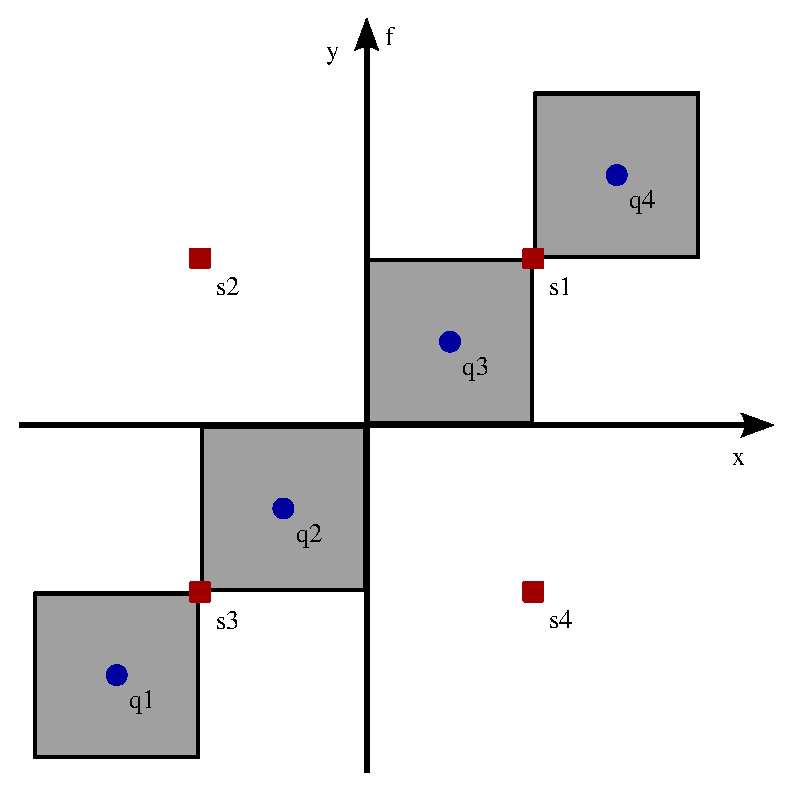
\epsfig{file=Figures/vectorquantizer,width=6cm}
\end{psfrags}
\caption{A visual graphical comparison of vector and scalar quantization schemes applied to the two-dimensional problem of Example~\ref{example:VectorQuantization}.}
\label{figure:VectorQuantizer}
\end{center}
\end{figure}
\end{example}

Although this example may not be the most realistic scenario, it provides a good illustration of the potential benefits associated with using vector quantizers.
The improved performance comes from the greater flexibility in positioning the various quantization points in a high-dimensional setting together with the ability to exploit correlation among consecutive source symbols.
On the downside, the mathematical treatment of a quantization problem becomes more intricate in a higher-dimensional space.


\section{Analysis-Synthesis Algorithms}

All the quantizers described up to this point are generic schemes designed to work well with abstract sources.
In practice, many quantization algorithms are tailored to specific applications.
These quantizers are called \emph{analysis-synthesis} coders, and their design is typically fairly intricate.
They require advanced models and are often evaluated according to complex performance metrics.
These criteria are rooted in human perception rather than conventional mathematics.
When developed properly, model-based quantization schemes achieve better compression ratios than the \emph{waveform coders} presented hitherto.
A serious treatment of analysis-synthesis algorithms is beyond the scope of this document.
Nevertheless, we mention two popular schemes below for illustrative purposes.

\paragraph{Speech Coding:}
The quantization mechanism employed in speech coding provides a nice example of an analysis-synthesis scheme.
Speech coders are widely used in mobile telephony and VoIP.
Human speech is modeled as a much simpler random process than most other audio signals, and there is an abundance of knowledge about its statistical properties and the way voice is generated.
As a result, some auditory information which is relevant in generic audio signals becomes inconsequential in the context of speech.
The primary performance criteria for voice signals are intelligibility and pleasantness of the received signal.
In addition, most speech applications require low delay, as long delays interfere with speech interaction in real-time applications.
The \emph{Code Excited Linear Prediction (CELP)} is a class of algorithms developed for human speech.
The basic idea behind this approach is to model human speech production using a time-varying linear filter.
The speech samples are subsequently separated in two distinct parts.
The first component contains the current parameters governing the operation of the linear filter; these parameters are selected from a finite set of possible values.
The second component captures the residual error, the difference between the predicted signal and the actual one.
This second signal is quantized using standard waveform coding techniques.
The overall operation of the system works quite well for conversations.
However, a speech coder applied to music fails to provide an adequate rendition of the original signal.

\paragraph{Joint Photographic Experts Group (JPEG):}
The JPEG algorithm is a file format designed to store photographs and paintings digitally.
The acronym JPEG is derived from the name of the committee that created this standard.
A JPEG file can actually be created in various ways.
A commonly used procedure specified in this standard is the \emph{JPEG file interchange format (JFIF)}, which we describe briefly.
The encoding process consists of several steps.
First, an image is represented using YCbCr, an encoding scheme that specifies every pixel (sample point) in the image according to a light intensity component (Y) and two chroma (Cb and Cr) for colors.
This scheme, as opposed to RGB, is interesting because it parallels the way the human visual system perceives image elements.
The image is then split into blocks of $8 \times 8$ pixels; and for each block, the Y, Cb, and Cr data undergoes a two-dimensional cosine transform.
This step is similar to a Fourier transform in the sense that it produces a spatial frequency spectrum.
The amplitudes of the resulting frequency components are quantized.
The resolution of the chroma data is reduced, compared to the light intensity component.
This reflects the fact that the human eye is less sensitive to fine color details than to fine brightness details.
Furthermore, human perception is much more sensitive to small variations in color or brightness over large areas than to the strength of high-frequency brightness variations.
Thus, the magnitudes of the high-frequency components are stored with a lower accuracy than the low-frequency components.
The resulting data for all $8 \times 8$ blocks is further compressed with a lossless algorithm, a variant of \emph{Huffman encoding}.
The important concept exposed in this example is how JPEG is built with a specific application in mind, and therefore quantizes sample data as to minimize the perceived distortion.
This is a very good illustration of an analysis-synthesis quantizer.



%\include{5ChannelCoding}
%\chapter{Waveform Communication}
\label{chapter:ContinuousTimeComm}

In Chapter~\ref{chapter:DiscreteTimeComm}, we introduced digital communication using a discrete-time model that allowed us to ignore the details of the more realistic continuous-time model.
The goal of this chapter is to delve into the details of waveform-based communication and see that the discrete-time model can be derived from the continuous-time model under some conditions.
The \defn{communication}{waveform channel} defines the probabilistic mapping between the deterministic channel input waveform $s(t)$ and the random-process $R(t)$ observed at the output of the channel.
The basic model is that $R(t) = s(t) + N(t)$, where $N(t)$ is Gaussian white-noise random process with autocorrelation function $R_N (\tau) = \delta(\tau) N_0 / 2$.
In some cases, the channel will also act as a linear filter and produce $R(t) = h(t) * s(t) + N(t)$, where $h(t)$ is the channel response.

\begin{figure}
\begin{center}
\begin{psfrags}
\psfrag{c}[c]{Channel}
\psfrag{x}[l]{$s(t)$}
\psfrag{n}[l]{$N(t)$}
\psfrag{r}[l]{$R(t)$}
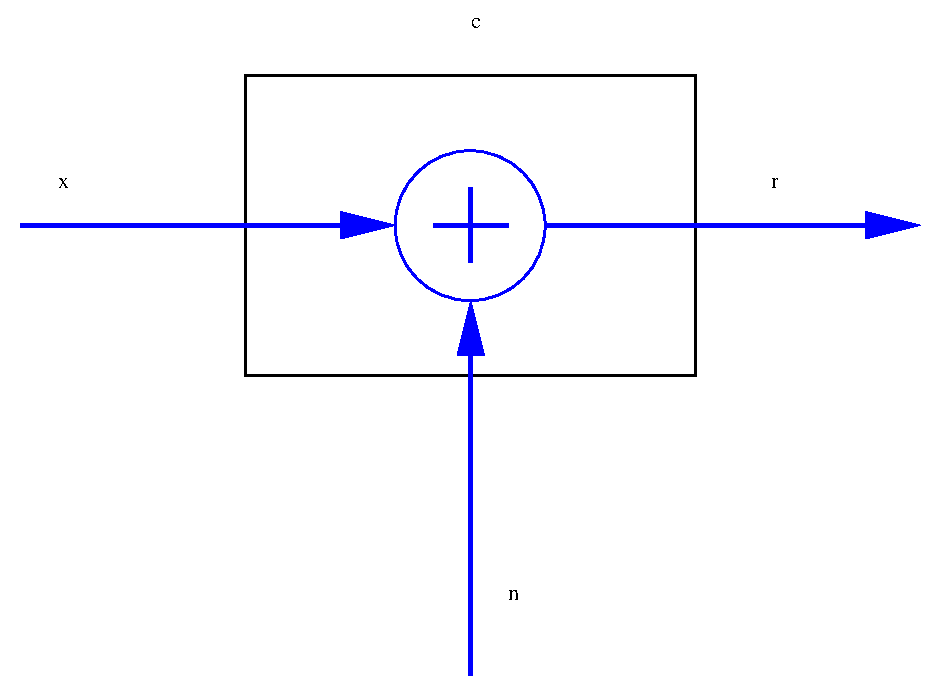
\epsfig{file=Figures/channel.eps,width=6.5cm}
\end{psfrags}
\end{center}
\caption{Block diagram of a basic waveform channel for input signal $s(t)$, noise process $N(t)$, and received signal $R(t)$.}
\end{figure}

\iffalse
\emph{Modulation} is the process by which a string of bits is converted into a signal suitable for transmission over a communication channel.
\emph{Demodulation} is the reverse operation at the destination where the information symbols are extracted from the received signal.
The shapes of the waveforms employed to create the transmitted signal are critical to the overall performance and operation of the system.
In many implementations, a high-frequency sinusoid is used, in addition to baseband pulse waveforms, as carrier to center the baseband signal at its intended frequency.
We initiate our study of modulation and demodulation with baseband signals; advanced considerations associated with carrier sinusoids and bandpass processes will be explored later.

Let $\{ s_k \in \{ 0, 1 \}^b \}$ be a sequence of binary symbols to be transmitted to a destination, and let $f : \{ 0, 1 \}^b \mapsto \mathbb{R}$ be an invertible function that takes a string of $b$ bits as input, and gives a real number as output, with $u_k = f(s_k)$.
Suppose further that several distinct waveforms are available at the transmitter, which we denote by $\{ \phi_k (t) \}$.
We study communication systems that modulate binary symbols in two steps.
First, a collection of binary data $\{ s_k \}$ is converted into a string of real numbers $\{ u_k \}$ using function $f(\cdot)$.
Next, these real numbers are used to form a transmission signal by creating a weighted linear combination of the basis functions,
\begin{equation*}
u(t) = \sum_k u_k \phi_k(t) .
\end{equation*}
This procedure provides a simple framework to transition back and forth between a digital sequence and the corresponding modulated signal.
At the destination, the sequence of binary symbols is demodulated by passing the received signal through linear time-invariant filters, and then mapping the resulting real number to one of the possible $b$-bit messsages.
\fi

\section{A Single Digital Symbol}

Suppose that one would like to send a single digital symbol taking $M$ different values to a receiver through a waveform channel.
Then, one can associate a waveform $s_m (t)$ with each symbol $m=1,\ldots,M$ and transmit the waveform assigned with the desired message.
For mathematical convenience, we assume that each waveform is zero outside of the interval $0\leq t\leq T$ where $T$ is symbol duration.

The demodulation process is based on mathematical operation, known as an inner product, that maps any two signals to a complex number.
The \defn{communication}{inner product} $\langle s(t) , r(t) \rangle$ between the signals $s(t)$ and $r(t)$ is defined by
\begin{equation*}
\left\langle s (t), r^* (t) \right\rangle
= \int_{-\infty}^{\infty} s(t) r^* (t) dt,
\end{equation*}
where $r^* (t)$ is the complex conjugate of $r(t)$.
Mathematically, we are treating the set of all finite-energy signals as a \defn{communication}{vector space} and using this inner product to define distances and angles in this space.
The energy (or length squared) of a signal $s(t)$ is given by
\[ \int_{-\infty}^{\infty} \left| s(t) \right|^2 dt = \langle s(t),s(t) \rangle. \]
Two signals $s_1 (t),s_2 (t)$ are said to be \defn{communication}{orthogonal} if $\langle s_1(t),s_2 (t)\rangle = 0$.
A signal $s(t)$ is said to be \textbf{normalized} if $\langle s(t),s(t) \rangle = 1$.
A set of signals is said to be \textbf{orthonormal} if every signal in the set is orthogonal to every other signal in the set and all signals in the set are normalized.
The set of all linear combinations of signal waveforms is called the \defn{communication}{signal space}.

\subsubsection{Orthonormal Waveforms}
The simplest scenario occurs when the set of signal waveforms $\{ s_1 (t), \ldots , s_M (t) \}$ is orthonormal.
In this case, one can demodulate the received signal $R(t)$ by computing
\[ R_j = \langle R(t), s_j (t) \rangle, \]
for each $j=1,\ldots,M$.
Due to the noise process, the resulting values $R_1 , \ldots, R_M$ are Gaussian random variables.
Their expected values depend on which waveform was actually transmitted.
If $s_m (t)$ was transmitted, then $R(t) = s_m(t) + N(t)$, $E[R(t)] = s_m(t)$, and we have
\begin{align*}
E \left[R_j \right]
&= E \left[ \int_{-\infty}^{\infty} R(t) s_j^* (t) dt \right] \\
&= \int_{-\infty}^{\infty} E \left[ R(t) \right] s_j^* (t) dt \\
&= \int_{-\infty}^{\infty} s_m (t) s_j^* (t) dt \\
&= \delta_{m,j}.
\end{align*}

The random variables $R_1, \ldots , R_M$ also have some other nice properties.
They are uncorrelated because the the waveforms are orthogonal and they have variance $N_0  / 2$ because the waveforms are normalized.
Proving this statement will be left as a homework exercise.

This transforms the waveform detection problem into a detection problem for a length-$M$ vector of Gaussian random variables.
If $s_m (t)$ was transmitted, then the mean of the random vector is the unit vector with a one in the $m$th position.
Based on the techniques from Chapter~\ref{chapter:DiscreteTimeComm}, the maximum-likelihood decision rule chooses the symbol whose unit vector is closest to the random vector $R_1,\ldots,R_M$ in Euclidean distance.

\begin{example}[Frequency-Shift Keying] \label{example:TSpacedTruncatedSinusoids}
For a fixed time-interval $T$, consider the collection of waveforms given by
\begin{equation*}
s_m(t) = \frac{1}{\sqrt{T}} e^{2 \pi i \frac{m}{T} t} \mathrm{rect} \left( \frac{t}{T} \right) .
\end{equation*}
for $m = 1, \ldots, M$.
This set of waveforms is known as $M$-ary frequency-shift keying (or $M$-FSK).
We wish to show that these waveforms are orthonormal.

To prove that they are orthogonal, we consider the inner product of $s_m(t)$ and $s_n(t)$ when $m \neq n$,
\begin{equation*}
\begin{split}
\left\langle s_m (t), s_n (t) \right\rangle
&= \int_{\mathbb{R}} s_m (t) s_n^* (t) dt 
= \frac{1}{T} \int_{-\frac{T}{2}}^{\frac{T}{2}}
e^{2 \pi i \frac{m}{T} t} e^{- 2 \pi i \frac{n}{T} t} dt \\
&= \frac{1}{T} \int_{-\frac{T}{2}}^{\frac{T}{2}}
e^{2 \pi i \frac{(m-n)}{T} t} dt
= 0 .
\end{split}
\end{equation*}
Next, we show that these basis elements have unit energy,
\begin{equation*}
\begin{split}
\left\| s_m(t) \right\|^2
&= \int_{\mathbb{R}} s_m (t) s_m^* (t) dt 
= \frac{1}{T} \int_{-\frac{T}{2}}^{\frac{T}{2}}
e^{2 \pi i \frac{m}{T} t} e^{- 2 \pi i \frac{m}{T} t} dt \\
&= \frac{1}{T} \int_{-\frac{T}{2}}^{\frac{T}{2}} dt
= 1 .
\end{split}
\end{equation*}
\end{example}

\subsubsection{General Waveforms}

When the signal waveforms are not orthonormal, the detection problem is solved most easily by constructing a set of orthonormal basis vectors for the signal space.
In general, this can be accomplished by applying the Gram-Schmidt orthogonalization process to the signal waveforms.
Rather than focusing on this process, we assume that $\{ \phi_1 (t), \ldots , \phi_N (t) \}$ is an orthonormal set of waveforms such that the coefficients $a_{m,k}$ allow us to write
\[ s_m (t) = \sum_{k=1}^N a_{m,k} \phi_k (t). \]
This implies that the orthonormal set spans the signal space.

In this case, the received signal $R(t)$ can be demodulated by computing
\[ R_j = \langle R(t), \phi_j (t) \rangle, \]
for each $j=1,\ldots,N$.
Again, the noise process implies that $R_1 , \ldots, R_N$ are Gaussian random variables whose means are determined by which waveform was actually transmitted.
For $j=1,\ldots,N$, the noise component of $R_j$ is independent of the transmitted signal, and is given by
\[ N_j = \int_{-\infty}^{\infty} N(t) \phi_j^* dt. \]
Therefore, $R_j = E[R_j] + N_j$ and the mean, if $s_m (t)$ was transmitted, is given by
\begin{align*}
E \left[R_j \right]
&= E \left[ \int_{-\infty}^{\infty} R(t) \phi_j^* (t) dt \right] \\
&= \int_{-\infty}^{\infty} E \left[ R(t) \right] \phi_j^* (t) dt \\
&= \int_{-\infty}^{\infty} s_m (t) \phi_j^* (t) dt \\
&= \int_{-\infty}^{\infty} \left( \sum_{k=1}^N a_{m,k} \phi_k (t) \right) \phi_j^* (t) dt \\
&= \sum_{k=1}^N a_{m,k} \delta_{k,j} dt \\
&= a_{m,j}. \\
\end{align*}

Again, we have transformed the waveform detection problem into a detection problem for a vector of Gaussian random variables.
In this case, however, there are $M$ different mean vectors of dimension $N$.
Based on the techniques from Chapter~\ref{chapter:DiscreteTimeComm}, the maximum-likelihood decision rule chooses the symbol $\hat{m}$ whose coordinate vector $(a_{\hat{m},1},\ldots. a_{\hat{m},N})$ is closest to the random vector $R_1,\ldots,R_N$ in Euclidean distance.

This approach can be seen as first projecting the infinite-dimensional received waveform onto a finite-dimensional subspace and then using the optimal detector on this finite-dimensional space.
To show that this overall approach is optimal, one must also prove that the residual waveform
\[ \tilde{N}(t) = R(t) - \sum_{j=1}^N R_j \phi_j (t) \]
does not contain any information relevant to the decision.
While this is indeed true, we ignore this detail for now.

\begin{figure}
\begin{center}
\begin{psfrags}
\psfrag{p1}[l]{$\phi_1(t)$}
\psfrag{p2}[l]{$\phi_2(t)$}
\psfrag{p3}[l]{$\phi_{N-1}(t)$}
\psfrag{p4}[l]{$\phi_N(t)$}
\psfrag{i}[c]{$\int_{0}^T (\cdot) dt$}
\psfrag{r}[l]{$r(t)$}
\psfrag{r1}[l]{$r_1$}
\psfrag{r2}[l]{$r_2$}
\psfrag{r3}[l]{$r_{N-1}$}
\psfrag{r4}[l]{$r_N$}
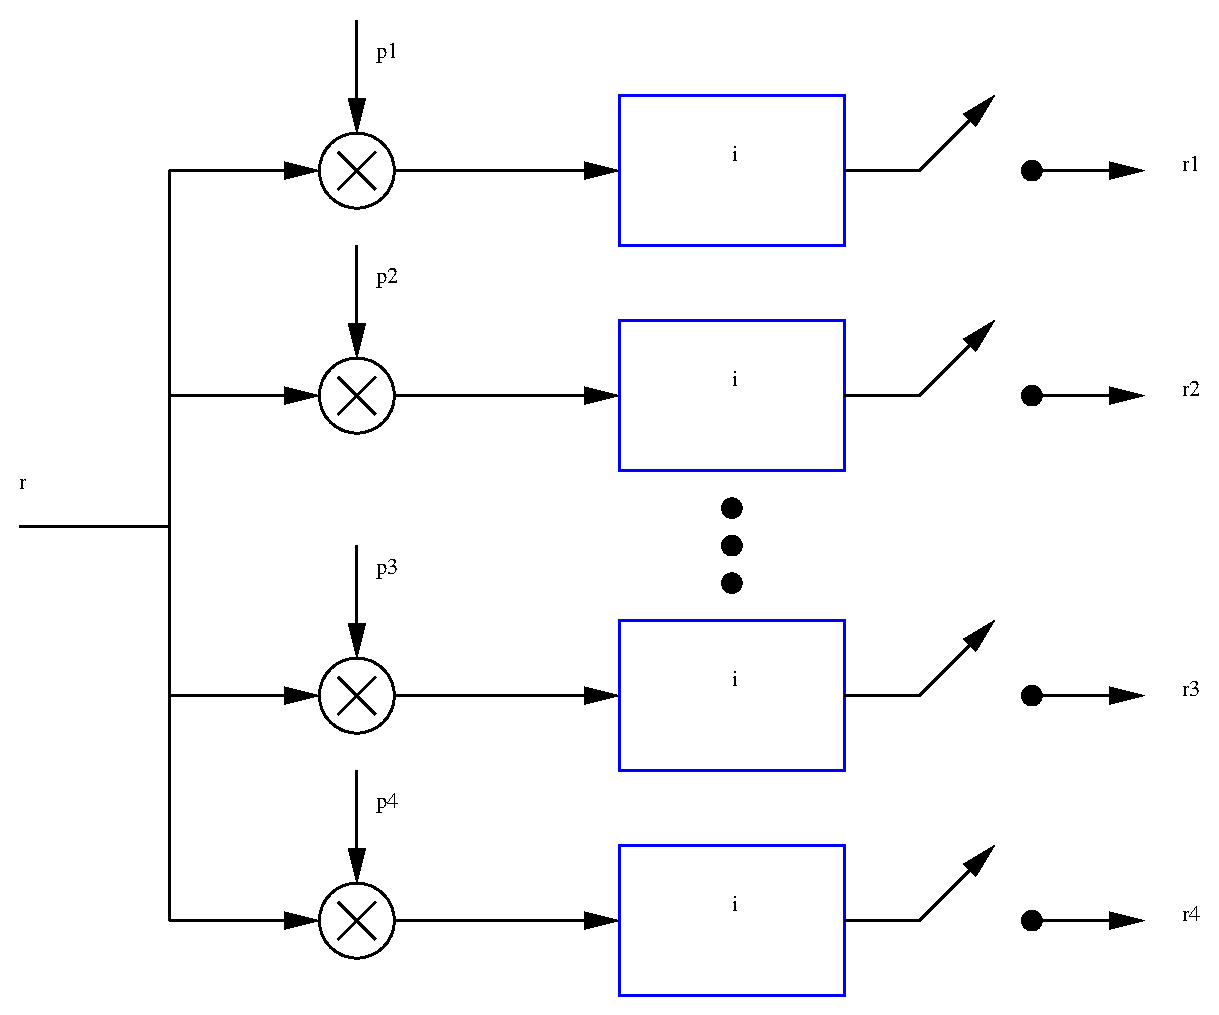
\epsfig{file=Figures/correlator.eps,width=8cm}
\end{psfrags}
\end{center}
\caption{For a particular realization $r(t)$ of the received signal, the received projection onto the signal-space basis vector can be computed by a bank of correlators.}
\end{figure}

\iffalse
The $T$-spaced truncated sinusoids of Example~\ref{example:TSpacedTruncatedSinusoids} form a collection of basis waveforms that can be employed to create a signal.
To further illustrate this point, we show explicitly how orthonormal waveforms can be used in the modulation and demodulation of data symbols.
Suppose that a signal is produced by taking a linear combination of the waveforms $\{ \phi_k(t) \}$, weighted by the real numbers $\{ u_k \}$, with
\begin{equation*}
u(t) = \sum_{k} u_k \phi_k(t) .
\end{equation*}
In the absence of noise, the original sequence of real numbers can be recovered at the destination using the projections afforded by the basis elements $\{ \phi_k (t) \}$.
In particular, we have
\begin{equation*}
\begin{split}
\left\langle u(t), \phi_n(t) \right\rangle
&= \int_{\mathbb{R}}
\left( \sum_{m=1}^M u_m \phi_m(t) \right) \phi_n^*(t) dt \\
&= \sum_{m=1}^M u_m \int_{\mathbb{R}}
\phi_m(t) \phi_n^*(t) dt
= u_n .
\end{split}
\end{equation*}

\begin{example}[Binary Modulation]
In this example, we consider the simplest possible scenario, the modulation of a single bit.
Suppose that a bit $s$ is mapped into the real numbers according to the rule
\begin{equation*}
u = f(s) = \begin{cases} -A, & s = 0 \\
A, & s = 1 , \end{cases}
\end{equation*}
where $A$ is a positive number and represents the amplitude of the waveform.
Then, the transmitted signal becomes
\begin{equation*}
u(t) = u \phi (t) .
\end{equation*}
To extract the value of $u$ for the signal $u(t)$, we simply compute the inner product of the signal with the basis element $\phi(t)$, which yields $u = \langle u(t), \phi(t) \rangle$.
The original bit $s$ is then obtained by taking the inverse of $u$ under function $f(\cdot)$, with $s = f^{-1} (u)$.
\end{example}

Except for noise considerations, this section presents the first principles under which modern digital communication systems operate.
Below, we continue our analysis of modulation and demodulation schemes by looking at the implications of sending multiple waveforms over time.
\fi

\section{Time-Shift Waveforms}

In practical communication systems, a succession of symbols is transmitted to the destination.
Not only can waveforms interfere with one another in signal space, they can also disrupt signal quality across time.
Suppose that a different symbol is sent every $T$ seconds using time shifts of a basic pulse waveform $p(t)$.
The transmitted signal, accounting for the different values of $\{ u_n \}$, is equal to
\begin{equation*}
u(t) = \sum_{n} u_n p (t - nT) .
\end{equation*}
Note that in this case, the available waveforms are simply translated versions of one another.
Ideally, we want the collection $\{ p(t - nT) \}$ to be orthonormal.
This would greatly simplify system implementation and decision making at the receiver.
However, we cannot use standard techniques such as the Gram-Schmidt procedure to construct a set of orthogonal waveforms, because the elements of $\{ p(t - nT) \}$ are constrained to be translated version of one another.
Getting an orthonormal set requires more work.

As before, each symbol $u_n$ is identified at the destination by passing the received signal through a linear time-invariant filter, which is mathematically equivalent to performing an inner-product integral.
Since the waveforms $\{ p(t-nT) \}$ are shifted versions of a same function, it is natural to expect the various filters to implement projections onto shifted versions of a single element $q(t)$.
A uniform treatment of the demodulation operation can therefore be conducted by looking a the inner product between $u(t)$ and $q(t-\tau)$.
Let
\begin{equation} \label{equation:InnerProductReceiver}
\begin{split}
r(\tau) &= \langle u(t), q(t-\tau) \rangle
= \int_{\mathbb{R}} u(t) q^*(t-\tau) dt \\
&= \sum_{k} u_k \int_{\mathbb{R}} p(t - kT) q^*(t-\tau) dt \\
&= \sum_{k} u_k g(\tau - kT) .
\end{split}
\end{equation}
where $g(\tau) = \langle p(t), q(t-\tau) \rangle$.
By convention, $q(t)$ is defined such that element $u_n$ is acquired by looking at $r(nT)$.
Rewritting \eqref{equation:InnerProductReceiver}, we get
\begin{equation*}
r(nT) = u_n g(0) + \sum_{k \neq n} u_k g((n - k)T) .
\end{equation*}
The first term in this expansion contains the desired symbols.
The remaining sum is called \emph{intersymbol interference (ISI)}; it contains the contributions from all the other time-shifted waveforms.
To retrieve the information sequence unambiguously, we wish to have $r(nT) = u_n$, irrespective of the values in the sequence $\{ u_k \}$.
This will be achieved provided that
\begin{equation} \label{equation:NoInterSymbolInterferenceSpecification}
g(nT) = \begin{cases} 1, & k = n \\
0, & \text{otherwise} . \end{cases}
\end{equation}
To understand how this condition impacts our choice of a functions $p(t)$ and $q(t)$, we use the frequency representation of $g(\tau)$.
Looking at the inverse Fourier transform of $\hat{g}(f)$, we get
\begin{equation*}
\begin{split}
g(\tau) &= \mathcal{F}^{-1} \left[ \hat{g} (f) \right]
= \int_{\mathbb{R}} \hat{g}(f) e^{2 \pi i f \tau} df \\
&= \sum_{m = -\infty}^{\infty} \int_{-\frac{F}{2}}^{\frac{F}{2}}
\hat{g} (f - Fm) e^{2 \pi i (f - mF) \tau} df
\end{split}
\end{equation*}
where, for reasons that will soon be obvious, we have judiciously selected $F = \frac{1}{T}$.
The value of $g(\tau)$ at the sample points $\{ \tau = nT : n \in \mathbb{Z} \}$ can then be expressed as
\begin{equation} \label{equation:SamplePointsNoISI}
\begin{split}
g(nT) &= \sum_{m = -\infty}^{\infty} \int_{-\frac{F}{2}}^{\frac{F}{2}}
\hat{g} \left( f - \frac{m}{T} \right) e^{2 \pi i \left( f - \frac{m}{T} \right) nT} df \\
&= \int_{-\frac{F}{2}}^{\frac{F}{2}}
\left( \sum_{m = -\infty}^{\infty} \hat{g} \left( f - \frac{m}{T} \right) \right)
e^{2 \pi i n T f} df \\
&= \frac{1}{F} \int_{-\frac{F}{2}}^{\frac{F}{2}}
\hat{z} (f) e^{2 \pi i \frac{n}{F} f} df ,
\end{split}
\end{equation}
where we have defined
\begin{equation*}
\hat{z}(f) = F \sum_{m = -\infty}^{\infty} \hat{g} \left( f - \frac{m}{T} \right)
\mathrm{rect} \left( \frac{f}{F} \right) .
\end{equation*}
Notice the similarity between \eqref{equation:SamplePointsNoISI} and the Fourier series representation of a time-limited function.
Specifically, $\{ g(nT) : n \in \mathbb{Z} \}$ can be viewed as the Fourier series coefficients of the frequency-limited function $\hat{z}(f)$.
Under condition \eqref{equation:NoInterSymbolInterferenceSpecification}, and using the reconstruction formula for Fourier series, we get
\begin{equation} \label{equation:NoInterSymbolInterference}
\hat{z}(f) = \sum_{n = -\infty}^{\infty} g(nT) e^{2 \pi i \frac{n}{F} f}
\mathrm{rect} \left( \frac{f}{F} \right)
= \mathrm{rect} \left( \frac{f}{F} \right)
\end{equation}
because $g(nT) = 0$ whenever $n \neq 0$.
Thus, the system exhibits no intersymbol interference if and only if \eqref{equation:NoInterSymbolInterference} holds.

Equivalently, condition~\eqref{equation:NoInterSymbolInterferenceSpecification} is satisfied whenever
\begin{equation} \label{equation:NyquistNoISI}
\sum_{m = -\infty}^{\infty} \hat{g} \left( f - \frac{m}{T} \right) = T .
\end{equation}
We formalize this key result, known as the \emph{Nyquist pulse-shaping criterion}, in the theorem below.

\begin{theorem}[Nyquist] \label{theorem:NyquistPulseCriterion}
Let $g(\tau)$ and $\hat{g}(f)$ be square integrable functions that are Fourier transforms of each other.
Furthermore, assume that the function
\begin{equation*}
\hat{z} (f) = F \sum_{m=-\infty}^{\infty} \hat{g} \left( f - \frac{m}{T} \right)
\mathrm{rect} (fT)
\end{equation*}
has finite energy.
Then, a necessary and sufficient condition for
\begin{equation*}
g(nT) = \begin{cases} 1, & n = 0 \\
0, & \text{otherwise} \end{cases}
\end{equation*}
is that the following equality holds for all values of $f \in \mathbb{R}$,
\begin{equation} \label{equation:NyquistCriterionFrequencyCondition}
\sum_{m=-\infty}^{\infty} \hat{g} \left( f - \frac{m}{T} \right) = T .
\end{equation}
\end{theorem}

\begin{example}
One of the simplest possible choices for waveforms $p(t)$ and $q(t)$ is
\begin{equation*}
p(t) = q(t) = \frac{1}{\sqrt{T}} \mathrm{rect} \left( \frac{t}{T} \right) .
\end{equation*}
In this case, we get
\begin{equation*}
\begin{split}
g(\tau) &= \langle p(t), q(t-\tau) \rangle
= \frac{1}{T} \int_{\mathbb{R}} \mathrm{rect} \left( \frac{t}{T} \right)
\mathrm{rect} \left( \frac{t - \tau}{T} \right) dt \\
&= \frac{1}{T} \int_{\mathbb{R}} \mathrm{rect} \left( \frac{t}{T} \right)
\mathrm{rect} \left( \frac{\tau - t}{T} \right) dt
= \frac{1}{T} \mathrm{rect} \left( \frac{t}{T} \right)
\ast \mathrm{rect}\left( \frac{t}{T} \right) .
\end{split}
\end{equation*}
Obviously, this selection leads to the desired property with $g(0) = 1$, and $g(nT) = 0$ for any non-zero integer~$n$.
One of the design issues with the rectangular pulse is that its bandwidth is infinite and decays slowly.
This becomes a problem in most practical systems where spectral bandwidth comes at a premium.
\end{example}

\begin{example}
Consider the pulse-shaping criterion applied to
\begin{equation*}
p(t) = q(t) = \frac{1}{\sqrt{T}} \mathrm{sinc} \left( \frac{t}{T} \right) .
\end{equation*}
We wish to show that this choice of waveforms satisfies the Nyquist criterion and leads to a set of orthogonal time-shift waveforms.

First, we find an expression for $g(\tau)$,
\begin{equation*}
\begin{split}
g(\tau) &= \langle p(t), q(t-\tau) \rangle
= \frac{1}{T} \int_{\mathbb{R}} \mathrm{sinc} \left( \frac{t}{T} \right)
\mathrm{sinc} \left( \frac{t - \tau}{T} \right) dt \\
&= \frac{1}{T} \int_{\mathbb{R}} \mathrm{sinc} \left( \frac{t}{T} \right)
\mathrm{sinc} \left( \frac{\tau - t}{T} \right) dt
= \frac{1}{T} \mathrm{sinc} \left( \frac{t}{T} \right)
\ast \mathrm{sinc} \left( \frac{t}{T} \right) .
\end{split}
\end{equation*}
In the frequency domain, we have
\begin{equation*}
\begin{split}
\hat{g}(f) &= \mathcal{F} \left[ g(\tau) \right]
= \frac{1}{T} \mathcal{F} \left[ \mathrm{sinc} \left( \frac{t}{T} \right) \right]
\mathcal{F} \left[ \mathrm{sinc} \left( \frac{t}{T} \right) \right] \\
&= T \mathrm{rect} (T f) \mathrm{rect} (T f)
= T \mathrm{rect} (T f) .
\end{split}
\end{equation*}
We can therefore verify condition~\eqref{equation:NyquistCriterionFrequencyCondition} as
\begin{equation*}
\sum_{m = -\infty}^{\infty}
\hat{g} \left( f - \frac{m}{T} \right)
= \sum_{m = - \infty}^{\infty} T \mathrm{rect} (Tf - m)
= T .
\end{equation*}
That is, the conditions of Theorem~\ref{theorem:NyquistPulseCriterion} hold and, consequently, $g(0) = 1$ and $g(n) = 0$ for any non-zero integer.
One of the positive attributes of the $\mathrm{sinc} (\cdot)$ waveform is that it is bandwidth-limited.
However, this pulse is not time-limited and it is therefore somewhat impractical, as using $\mathrm{sinc} (\cdot)$ waveforms would entail infinite delay at the destination.
\end{example}

Although, there are many choices for $\hat{g}(f)$ that satisfy Theorem~\ref{theorem:NyquistPulseCriterion}, we are primarily interested in waveforms that are approximately both bandwidth-limited and time-limited.
The \emph{Nyquist bandwidth} associated with a signal
\begin{equation*}
u(t) = \sum_k u_k p(t -kT)
\end{equation*}
is defined by $\frac{1}{2T}$; it represents the smallest possible bandwidth for which it is possible to prevent intersymbol interference.
The spectral bandwidth of $\hat{g}(f)$ is the smallest possible value of $W$ such that $\hat{g}(f) = 0$ for $|f| > W$.

\iffalse
\subsection{Pulse Amplitude Modulation}

Pulse amplitude modulation (PAM) is a simple form of modulation, where data is embedded in the amplitude of a single waveform,
\begin{equation*}
u(t) = u \phi (t) .
\end{equation*}
The incoming binary data is segmented into binary symbols of $b$ bits, and each block is mapped into one of $2^b = M$ possible real numbers within the constellation set $\mathcal{A} = \{ a_1, \ldots, a_M \}$.
In the absence of noise and interference, the value of the sent $b$-bit message is recovered by first taking the inner product of $u(t)$ with the basis element $\phi (t)$,
\begin{equation*}
u = \langle u(t), \phi(t) \rangle = \int_{\mathbb{R}} u(t) \phi^*(t) dt ,
\end{equation*}
and then extracting the original $b$ bits from $u$, using the inverse map.
In standard $M$-PAM, where $M = 2^b$, the amplitude set is equal to
\begin{equation*}
\mathcal{A} = \left\{ - \frac{d(M-1)}{2} , \ldots, - \frac{d}{2}, \frac{d}{2}, \ldots, \frac{d(M-1)}{2} \right\} ,
\end{equation*}
and $d$ denotes the distance between adjacent points.

\subsection{Quadrature Amplitude Modulation}

A closely related modulation scheme is quadrature amplitude modulation (QAM).
In this scheme, data is conveyed to the destination by changing the amplitude of two carrier waves.
Equivalently, QAM can be interpreted as modulating a compex amplitude onto a single waveform,
\begin{equation*}
u(t) = (u + iv) \phi(t) .
\end{equation*}
In both cases, the space spanned by $u(t)$ is two-dimensional (over the real numbers), and the constellation can be abstracted to $\mathcal{A} = \{ (a_1, b_1), \ldots, (a_M, b_M) \}$ where $M = 2^b$ as before.
In a noiseless environment, the modulating scalar $u + iv$ can be extracted from $u(t)$ using the inner product
\begin{equation*}
u + i v = \left\langle u(t), \phi(t) \right\rangle .
\end{equation*}
Note that we can write the received signal in vector form as
\begin{equation*}
(u, v) = \left( \Re \left( \left\langle u(t), \phi(t) \right\rangle \right),
\Im \left( \left\langle u(t), \phi(t) \right\rangle \right) \right) .
\end{equation*}
The latter interpretation, where QAM is seen as a single waveform modulated by a complex number, originates from the fact that baseband waveforms are often modulated by sinusoid carriers.
The in-phase ($\cos (2 \pi f_{\mathrm{c}} t)$) and quadrature ($\sin (2 \pi f_{\mathrm{c}} t)$) components of the bandpass signal then correspond to the real and imaginary parts of the baseband waveform.

\begin{example}[Phase Shift Keying]
In phase shift keying (PSK), the transmitted signal $u(t)$ is given by
\begin{equation*}
u(t) = \frac{1}{\sqrt{T}} e^{2 \pi i f_{\mathrm{c}} t + i \theta}
\mathrm{rect} \left( \frac{t}{T} \right) ,
\end{equation*}
where $\theta$ is one of finitely many possibility and the carrier freqency $f_{\mathrm{c}}$ is an integer multiple of $\frac{1}{T}$.
The data in PSK is embedded in $\theta$, the phase of the sinusoid.
Note that the function $u(t)$ can be rewritten as
\begin{equation*}
\begin{split}
u(t) &= e^{i \theta} \frac{1}{\sqrt{T}} e^{i (2 \pi f_{\mathrm{c}} t + \theta)}
= \left( \cos (\theta) + i \sin (\theta) \right) \phi (t) \\
&= (u + iv) \phi (t) .
\end{split}
\end{equation*}
That is, the signal constellation in PSK is constrained to lie on the unit circle.
\end{example}



\newpage

\section{Transmitting symbols over Time}

\subsection{Orthogonality in Time}

\subsection{The Nyquist Criterion}
HERE

\newpage

\section{High-Dimentional Signal Constellations}

\subsection{Orthogonal Signal Waveforms}

\subsection{Simplex Signal Waveforms}

\subsection{Bi-Orthogonal Signal Waveforms}


\section{Signal Space Representation}

Let $\mathcal{W} = \{ \phi_1 (t), \ldots, \phi_D (t) \}$ be an orthonormal set of functions.
Furthermore, suppose that this set possesses the following property,
\begin{equation*}
\left\langle \phi_m \left( t - \frac{k}{T} \right),
\phi_n \left( t - \frac{l}{T} \right) \right\rangle
= \int_{\mathbb{R}} \phi_m \left( t - \frac{k}{T} \right)
\phi_n^* \left( t - \frac{l}{T} \right) dt 
= 0
\end{equation*}
for all $k, l, m, n \in \mathbb{Z}$, except cases where $k = l$ and $m = n$.


\begin{example}[$T$-spaced sinc functions]
This time, let
\begin{equation*}
\phi_m(t) = \frac{1}{\sqrt{T}} e^{-2 \pi i \frac{m}{T} t} \mathrm{sinc} \left( \frac{t}{T} \right)
\end{equation*}
\end{example}



Furthermore, the energy of the transmitted waveform depends on the value of $A$,
\begin{equation*}
\| u(t) \|^2 = \| u_1 \phi_1 (t) \|^2 = |u_1|^2 \| \phi_1(t) \|^2 = A^2 .
\end{equation*}
Naturally, the larger the amplitude is, the greater the energy of the signal becomes.
\section{Detection}

\section{Synchronization}

When the incoming bits are independent, each with equal probabilities of being zero or one, the transmitted waveform becomes a stochastic signal $U(t) = U \phi(t)$.
We can compute the energy of this random waveform $U(t)$ as
\begin{equation*}
\begin{split}
E_{\mathrm{s}} &= \mathrm{E} \left[ \int_{\mathbb{R}} |U(t)|^2 dt \right]
= \mathrm{E} \left[ U^2 \right] \| \phi (t) \|^2 \\
&= \sum_{m=1}^M \frac{1}{M} \frac{(2m - M - 1)^2 d^2}{2} \\
&= \frac{\left( M^2 - 1 \right) d^2}{12} .
\end{split}
\end{equation*}
That is, the average energy used per transmitted symbol is $\frac{(M^2 - 1) d^2}{12}$ and, correspondingly, the average energy per bit is
\begin{equation*}
E_{\mathrm{b}} = \frac{ E_{\mathrm{s}} }{M}
= \frac{\left( M^2 - 1 \right) d^2}{12M}
= \frac{\left( 2^{2b} - 1 \right) d^2}{12 \cdot 2^b} .
\end{equation*}
Roughly speaking, for large PAM constellations, the energy consumption per bit doubles with every additional bit.


\subsection{Linear Time-Invariant Filters and Inner Products}

\fi



\appendix

%\include{A0VectorSpaces}

%\include{fdl}

\backmatter

\printindex

\end{document}
